\documentclass[11pt, letterpaper]{article}

% === PACKAGES FOR BETTER LAYOUT AND TYPOGRAPHY ===
\usepackage[utf8]{inputenc}
\usepackage[english]{babel}
\usepackage{graphicx}
\usepackage{hyperref}
\usepackage{caption}
\usepackage{float}
\usepackage[margin=1in]{geometry}
\usepackage{subcaption}

% --- Font & Typography ---
\usepackage{lmodern}         
\usepackage{microtype}       


% --- Page Layout & Spacing ---
\usepackage[margin=1in]{geometry} % Set 1-inch margins.
\usepackage[parfill]{parskip}     % Use vertical space between paragraphs instead of indentation.

% --- Headers & Footers ---
\usepackage{fancyhdr}        % For custom headers and footers.
\pagestyle{fancy}
\fancyhf{} % Clear all header and footer fields
\fancyhead[L]{\nouppercase{\leftmark}} % Current section title on the left
\fancyfoot[C]{\thepage} % Page number in the center footer
\renewcommand{\headrulewidth}{0.4pt}
\renewcommand{\footrulewidth}{0pt}

% --- Math, Graphics, and Tables ---
\usepackage{amsmath}         % For advanced math environments
\usepackage{graphicx}        % For including images
\usepackage{booktabs}        % For professional-looking tables
\usepackage{float}           % For improved figure placement control with [H]
\usepackage{tabularx}        % For tables with auto-wrapping text columns

% --- Caption Control ---
\usepackage{caption}         % For customizing captions
\captionsetup{font=footnotesize, justification=centering}

% --- Hyperlinks & Referencing ---
\usepackage{url}             % For formatting URLs
\usepackage{hyperref}        % For clickable links and references
\hypersetup{
    colorlinks=true,
    linkcolor=blue,
    filecolor=magenta,      
    urlcolor=cyan,
    pdftitle={Analysis of Cardano's stake pool incentive mechanism},
    pdfauthor={Carlos Lopez de Lara},
}

% --- Table of Contents Control ---
\usepackage{tocbibind}       % Automatically adds Table of Contents, etc., to the ToC itself.

% --- Numbering Control ---
\setcounter{secnumdepth}{3} % Number sections, subsections, and subsubsections.

% === DOCUMENT METADATA ===
\title{Analysis of Cardano's stake pool incentive mechanism}

\author{
    Carlos Lopez de Lara \\
    Input Output Engineering \\
    \texttt{carlos.lopezdelara@iohk.io}
}

\date{October 20, 2025}

% === Start new sections in new pages ===
\usepackage{titlesec}
\newcommand{\sectionbreak}{\clearpage}

\usepackage{makecell}


% === DOCUMENT START ===
\begin{document}

\begin{titlepage}
    \centering % Center all content
    
    \vfill % Pushes the title down from the top
    
    % --- TITLE ---
    {\Huge \textbf{Analysis of Cardano's incentive mechanism}}
    
    \vfill 
    
    {
        \Large \textbf{Carlos Lopez de Lara} \\
        \vspace{1em} 
        \large Input Output Engineering \\
        \large \texttt{carlos.lopezdelara@iohk.io}
    }
    
    \vfill
    
    {\large October 20, 2025}
    
    \vfill 
\end{titlepage}

\thispagestyle{empty} 

\tableofcontents
\newpage
\pagestyle{fancy} 

\newpage

\section*{Acknowledgements}

The author wishes to express sincere gratitude to the individuals whose 
invaluable insights and detailed feedback were instrumental to this work: 
\textbf{Samuel Leathers, Alejandro Garcia, Arturo Mora, Evangelos Markakis, Ryan Wiley, 
Matthew Capps, and Rich Manderino}.

Special thanks are extended to \textbf{Kevin Hammond, Neil Davis, Alexander Moser, Markus Gufler, 
Vijayanath Bhuvanagiri and Adam Rusch} from the Intersect Protocol Parameters Sub-Committee for 
their support and technical discussions; and to \textbf{Taichi Yokoyama}, who played a critical role in
facilitating and translating workshops with the Japanese SPO community.

To the \textbf{SPO community} that registered and took part in the focus groups, your candid 
feedback and operational experiences were vital to grounding this analysis in real-world conditions
and to better understanding the motivations and challenges faced by operators: \textbf{Atlas, banC, Bastian - SHARE, 
Baudouin Muvunga, Bernard Sibanda, BTBF, Cassandra de Vries, Chad - BBHMM, Chris - STR8, 
David Airebamen, Delon Wenyeve, ERT\"URK G\"URBOGA, Fergie Miller, Jeremy, Jesse Smith, Lauri, Leon - HAPPY, 
Markus Gufler, MUEN, Nekota - NAP, Nils Codes, Rodrigo - CHIL, Shane Lazar, Shawn McMurdo, 
shiodome47, Star Forge, Stef - RABIT, Rich Manderino, Tatsuro Kyoden, GAIN, NAP, AICHI, ATRMN, ADA1, BTBF, AIRX,
CTEC, d-san, Daikon, Daisuke, Genhen, RX78, kpcn, MUEN, MUGEN, n\_oyaji, NNSP, Rakuda, Shiodome, TGEM, STARO, Taro,
USAGI, YYZ, z-dev.ai, ASY, Taireru, SASA, Tammy, KAP, ISPF}. Their perspectives enriched the qualitative dimension of this
report. Best wishes to all for continued success in your stake pool endeavors.

Finally, a special acknowledgment is due to the original designers of the incentive scheme: 
\textbf{Philipp Kant, Lars Brünjes, and Duncan Coutts}. Time has proven their design to be fundamentally 
sound and robust, successfully guiding rational actors so that their self-interested behavior results in 
optimal outcomes for the security and efficiency of the protocol.

\newpage

% === EXECUTIVE SUMMARY START ===

\section*{Executive Summary}

This report provides a comprehensive analysis of Cardano's incentive mechanism, five years after its 
launch in the Shelley era. The primary objective is to evaluate the system's real-world performance 
against its original game-theoretic design goals, assessing its overall health, identifying systemic 
risks, and determining the need for protocol adjustments. The methodology compares the theoretical goals 
codified in the design specification (Section 2) with a deep empirical analysis of on-chain data and 
qualitative findings from Stake Pool Operator (SPO) focus groups (Section 3).

\subsection*{Key Findings}

The analysis reveals a system of dual outcomes: the incentive mechanism is a resounding technical 
success in securing the network, while simultaneously creating significant socio-economic challenges 
for its operator community.

\begin{itemize}
    \item \textbf{A secure and performant network:} The core goals of incentivizing participation and 
    performance have been unequivocally met. The network is robustly decentralized and secure, supported by 741 
    "Healthy" pools and 246 "Viable" pools, and consistently achieves over 98\% of its theoretical maximum block 
    production.
    
    \item \textbf{Flawless protocol mechanics:} The automated rewards distribution system has functioned 
    flawlessly since inception, validating its design. Furthermore, the pledge mechanism is proven to be a 
    highly effective Sybil deterrent, creating a powerful economic incentive to consolidate capital, just as it 
    was designed to do.
    
    \item \textbf{The "Paradox of Pledge":} While an effective Sybil deterrent, the pledge mechanism 
    fails as a meaningful "skin-in-the-game" signal for the vast majority of operators. On-chain analysis 
    confirms the reward bonus is "functionally irrelevant" for pledges under 10M ADA (e.g., deltas as low 
    as 0.07 ADA), a finding echoed by frustrated SPOs. This creates a competitive imbalance that primarily 
    benefits well-capitalized actors.
    
    \item \textbf{The "Viability gap":} The system has not converged on the theoretical $k=500$ pools, but 
    has instead found a stable, stratified equilibrium of 1,614 active pools. A direct consequence is the 
    "viability gap": 873 active operators (54\% of the total) remain below the 3M ADA threshold required for 
    consistent block production.
    
    \item \textbf{A Capital-constrained environment:} The viability gap is cemented by two real-world factors 
    not accounted for in a simplified rational-actor model. First, approximately 16B ADA remains outside the 
    consensus mechanism, creating a capital-constrained, zero-sum environment. Second, delegator behavior is 
    complex, dominated by inertia ("sticky stake") rather than pure yield optimization.
\end{itemize}

\subsection*{Risks and Conclusions}

The report identifies two primary risks to the network:

\begin{enumerate}
    \item \textbf{High social risk:} The most immediate threat is operator disillusionment. The "viability gap" 
    and the pledge paradox have created a large, disenfranchised segment of the operator community that feels the 
    system is inequitable.
    
    \item \textbf{Long-term economic risk:} The network's sustainability model is contingent on a successful 
    transition from the current reward system, which is overwhelmingly subsidized by the depleting ADA reserves,
    to one funded by transaction fees. This places immense importance on the Leios upgrade and the ecosystem's 
    ability to generate "killer apps" that drive sustainable on-chain activity.
\end{enumerate}

The findings indicate that the system requires \textbf{fine-tuning and targeted revisions, not a complete overhaul}. The fundamental game-theoretic model is sound for its primary purpose of securing the network.

\subsection*{Recommendations}

The report proposes a multi-pronged approach for consideration by governance and protocol developers:

\begin{itemize}
    \item \textbf{Address the viability gap:} Explore new on-chain mechanisms, such as "pool alliances" or "virtual pools," to allow the 873 struggling operators to combine resources and compete effectively.
    
    \item \textbf{Re-evaluate parameters:} Formally analyze and debate adjustments to economic parameters, including a minimum margin and a reduction of the fixed cost, to address operator frustrations.

    \item \textbf{Consider minPoolMargin:} This proposal seems to have the support from pools of all sizes. Should be paired with a reduction of minPoolCost to 0. Researchers think minPoolCost favors Sybil attacks.

	\item \textbf{Prune inactive pools:} Initiate a formal research effort to define an on-chain mechanism for pruning the 1,305 "Inactive" pools, addressing the "stale stake" problem.

    \item \textbf{Activate latent stake:} Launch a formal research initiative to understand the barriers preventing 16 billion ADA from participating in consensus.
\end{itemize}

% === EXECUTIVE SUMMARY END ===
\newpage
\section{Introduction}

\subsection{Background and motivation}
Five years have passed since the Cardano blockchain's transition to the Shelley
era, a shift from a federated network to a decentralized Proof-of-Stake (PoS)
model. Central to this model is delegation, which allows any holder of the
network's native asset, ada, to participate in the protocol's consensus
mechanism by delegating their stake to Stake Pools. This is essential for
network security and performance.

The success of this decentralized ecosystem depends on its incentive mechanism.
This mechanism is the economic engine designed to align the financial
self-interest of rational actors—both delegators and SPOs—with the long-term
health, security, and decentralization of the network. The design, as detailed
in the \textit{\textbf{Shelley-era Delegation and Incentives Design
		Specification (SL-D1)}}, is built on game-theoretic principles that predict how
participants will behave under a specific set of economic rules. Now, after
five years of operation, a body of on-chain data and operational experience
exists. This allows for an empirical analysis of the scheme's real-world
effectiveness. The question is no longer whether the incentives \textit{will}
function as predicted, but whether they \textit{have}. This report provides a
review to bridge the gap between the intended design and the observed on-chain
outcomes, assessing its performance and identifying areas for potential
refinement.

\subsection{Scope and primary objectives}
This report assesses the economic health and performance of Cardano's stake
pool incentive scheme. The analysis is grounded in the goals and mechanisms
outlined in the design specifications, primarily the \textit{Shelley-era
	Delegation and Incentives Design Specification (SL-D1)}. The scope of this
report is defined by three objectives:

\begin{itemize}
	\item To determine if the current incentives scheme has been successful in achieving
	      its stated goals, with these goals being derived directly from the design
	      specification.
	\item To determine, based on the findings of the initial analysis, whether the system
	      requires minor parameter adjustments (fine-tuning), a more significant revision
	      of its mechanisms (overhaul), or if the current configuration is performing
	      optimally.
	\item To determine if the current scheme presents systemic risks to the long-term
	      health and security of the network. This includes an assessment of whether
	      stake pool operators have sufficient incentive to continue securing the
	      protocol into the future.
\end{itemize}

\subsection{Methodology and report structure}
To achieve these objectives, this report follows a three-phase analytical
approach that moves from theory to practice and finally to synthesis.
\begin{itemize}
	\item \textbf{Phase 1: Foundational analysis.} The first phase involves a review of the design
	      specification (SL-D1) to codify the system's intended goals, its predictions out actor behavior, and
	      the mechanics of the rewards system. This creates a theoretical benchmark against which the live
	      network can be measured.
	\item \textbf{Phase 2: Empirical analysis.} The second phase tests the theoretical model against reality.
	      This involves analyzing quantitative on-chain data to measure network outcomes such as decentralization,
	      stake distribution, and delegator behavior. This data is supplemented with qualitative findings from
	      focus groups with Stake Pool Operators to understand the motivations behind the observed trends.
	\item \textbf{Phase 3: Synthesis and evaluation.} The final phase compares the theoretical design from
	      Phase 1 with the empirical results from Phase 2. This is used to draw conclusions, directly address
	      the three objectives, identify systemic risks, and formulate final recommendations.
\end{itemize}
The report is structured to follow this methodology. Section 2 summarizes the design of the incentive
mechanism. Section 3 presents the empirical analysis of on-chain data. Section 4 synthesizes these findings
to evaluate the system's performance, followed by final conclusions and recommendations in Section 5.

\section{Foundational analysis: goals of the incentives design}
The design of the Cardano incentives scheme intends to align the financial
self-interest of individual actors with the overall health, security, and
decentralization of the network. An analysis of the \textit{Shelley-era
	Delegation and Incentives Design Specification} reveals a set of core goals and
behavioral predictions that form the theoretical foundation of the economic
model.

\subsection{Design goals}
The delegation design is intended to produce a specific set of behaviors and
system properties:
\begin{itemize}
	\item \textbf{System equilibrium:} The mechanism is designed to guide the ecosystem toward a stable state
	      where a majority of stake is delegated to a target number of pools, \textbf{$k$}, preventing the
	      centralization that could arise from a few dominant pools.
	\item \textbf{Performance and participation:} Rewards are structured to incentivize operators to fulfill
	      their protocol responsibilities, namely consistent block production and providing reliable network
	      infrastructure.
	\item \textbf{Automatic and efficient rewards:} Reward sharing is an automatic protocol function that does
	      not require manual intervention from operators or members. The process is designed to avoid excessive
	      growth of the UTXO set or transaction bursts that could compromise network performance.
	\item \textbf{Sybil resistance:} The mechanism is designed to discourage \textbf{Sybil attacks}, where an
	      adversary creates many pools to gain disproportionate influence. This is primarily addressed through the
	      \textbf{pledge} mechanism, which rewards owners for committing their own capital (``skin in the game''),
	      making it uneconomical to create numerous low-quality pools.
	\item \textbf{Cooperative behavior:} The monetary expansion formula is dependent on the total number of
	      blocks produced in an epoch, which is designed to incentivize cooperative behavior and discourage pools
	      from sabotaging each other's blocks.
\end{itemize}

\subsection{The rewards calculation mechanism}

The rewards calculation is the mechanism through which the incentive structure
is materialized. A stake pool's ability to earn rewards depends on structural
and operational factors. Structurally, its total stake ($\sigma$) and owner's
pledge ($s$) determine its theoretical reward cap, with both values constrained
by the saturation point ($z_{0}$). The system rewards operators who commit more
personal stake through the pledge influence factor ($a_{0}$), while capping
benefits for oversaturated pools to promote decentralization. Operationally,
actual rewards are gated by performance ($\bar{p}$); only pools that produce
blocks receive rewards. Additionally, pools must meet their declared pledge to
qualify for any rewards. The distribution mechanism ensures operator costs and
margins are prioritized before delegators are paid. Together, these parameters
align incentives around decentralization, reliability, and operator commitment.

\begin{enumerate}
	\item \textbf{The epoch reward pot ($R$) is determined.} Before individual pool rewards are calculated, a
	      total amount of rewards available for the epoch is established. This pot is sourced from transaction fees
	      collected during the epoch (\texttt{fees}) and a percentage ($\rho$) of the remaining ADA in the reserves
	      (\texttt{reserves}). The calculation proceeds as follows:
	      \begin{enumerate}
		      \item Calculate monetary expansion: \[ \text{Monetary Expansion} = \rho \cdot \text{reserves} \]
		      \item Calculate total potential rewards:
		            \[ \text{Total Potential Pot} = \text{fees} + (\rho \cdot \text{reserves}) \]
		      \item Calculate the final reward pot (R):
		            \[ R = (1 - \tau) \cdot (\text{fees} + \rho \cdot \text{reserves}) \]
	      \end{enumerate}
	      This value $R$ is the total ADA available to be shared among all stake pools in a given epoch.

	\item \textbf{A pool's optimal reward is calculated.} The protocol calculates the maximum potential reward
	      a pool is entitled to, assuming perfect performance. The formula is:
	      \[ f(s, \sigma) := \frac{R}{1+a_0} \cdot
		      \left(\sigma' + s' \cdot a_0 \cdot \frac{\sigma' - s' \frac{z_0 - \sigma'}{z_0}}{z_0}\right) \]
	      The formula uses $\sigma' = \min(\sigma, z_0)$ and $s' = \min(s, z_0)$. This is
	      the mechanism that enforces the saturation point. Any stake a pool controls
	      beyond the saturation point ($z_{0}$) is ignored for the reward calculation.

	\item \textbf{Rewards are adjusted for performance.} The optimal reward is a theoretical maximum. This value
	      is multiplied by the pool's apparent performance ($\bar{p}$). The actual reward $\hat{f}$ being:
	      \[ \hat{f}(s, \sigma, \bar{p}) := \bar{p} \cdot f(s, \sigma) \]

	\item \textbf{The final reward is distributed to stakeholders.} Once a pool's final, performance-adjusted
	      reward ($\hat{f}$) is calculated, it is split according to its declared parameters. If a pool's owners fail
	      to meet their declared pledge in an epoch, the pool earns zero rewards for that epoch. If the pledge is met,
	      the reward is distributed as follows:
	      \begin{itemize}
		      \item First, the fixed cost ($c$) is subtracted and given to the operator.
		      \item Second, the percentage margin ($m$) is calculated from the remainder and also
		            given to the operator.
		      \item Finally, all remaining rewards are distributed proportionally among all
		            delegators (including the pool owner's pledge) based on their stake
		            contribution.
	      \end{itemize}
\end{enumerate}

\section{Empirical analysis: on-chain outcomes vs design goals}

This section tests the theoretical design goals from Section 2 against real-world
outcomes by analyzing on-chain data and various aspects of the stake pool ecosystem.

\subsection{Determining the economic viability threshold}

A sustainable, decentralized network requires that stake pool operations are
economically viable. This means operators should not be forced to subsidize infrastructure
with external capital, which is an unstable long-term condition.

Establishing a definitive viability threshold is a primary analytical challenge. Operational
costs vary significantly with infrastructure, geography, and scale. Volatility between fiat-denominated
costs and ADA-denominated rewards adds to this complexity. Our methodology addresses these variables by
establishing a baseline cost profile derived from empirical data.

This cost model is derived from an analysis of on-demand pricing from major
cloud service providers (AWS, Google Cloud, Digital Ocean) for a standard
three-node topology (\textbf{one block producer, two relays}). The analysis
establishes a baseline operational expenditure of approximately \textbf{\$667
	USD per month}, accounting for compute, network, and storage costs. This
baseline was validated by cross-referencing against cost data reported by a
sample of stake pool operators, who reported expenditures ranging from \$150 to
\$1200 USD per month. Therefore, the \$667 figure seems like a reasonable
estimate for the median cost of a professionally managed operation.

To denominate this fiat cost in ADA, we employ the average ADA/USD exchange
rate from the preceding six-month period (April 2025 – September 2025), which
stands at \$0.71. This timeframe was selected to provide a contemporary
valuation while mitigating the effects of short-term market volatility.

\begin{figure}[H]
	\centering
	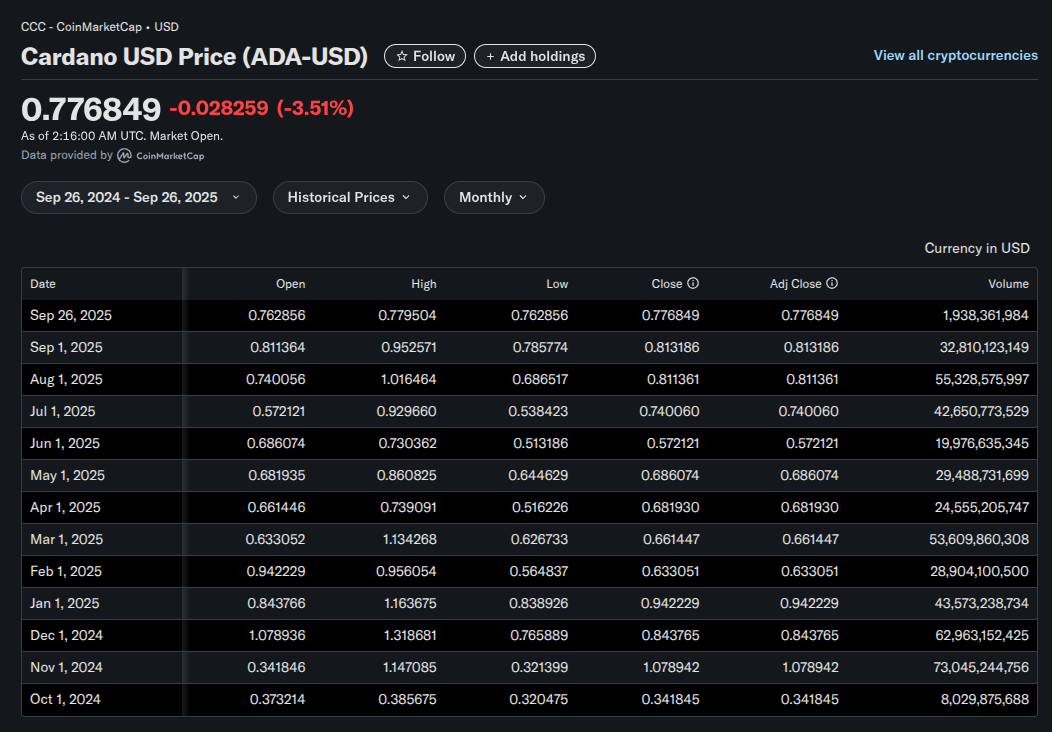
\includegraphics[width=0.8\textwidth]{img/ada-usd.png}
	\caption{ADA/USD price, April 2025--September 2025. Source: CoinMarketCap.}\label{fig:ada-price}
\end{figure}

This gives an equivalent operational cost in ADA, calculated per epoch (5
days):

\[ \text{Cost per Epoch (ADA)} =
	\frac{\text{Monthly Cost (USD)} / (\frac{30\text{ days}}{5 \text{ days/epoch}})}{\text{Average ADA Price (USD)}}
	= \frac{\$667 / 6}{\$0.71} \approx 156\text{ ADA} \]

This figure of \textbf{156 ADA per epoch} serves as the benchmark for
evaluating stake pool viability.

It must be noted that this fiat-denominated cost basis subjects all operators
to exchange rate volatility. A sustained depression of the ADA/USD exchange
rate represents a systemic risk, as it could render pools operating near the
viability threshold unprofitable. While this analysis acknowledges this market
exposure, its scope does not include exchange rate forecasting. The benchmark
of 156 ADA is therefore established as a point-in-time metric, intended to
provide a stable baseline for evaluating the current economic state of the pool
ecosystem.

A pool's economic viability is contingent upon its ability to generate rewards
by consistently producing blocks. This analysis defines ``consistency'' as a
95\% probability of producing at least one block per epoch. The corresponding
stake required to meet this threshold is derived from a binomial probability
model.

\begin{enumerate}
	\item \textbf{Inputs}
	      \begin{itemize}
		      \item $S=432,000$ (slots per epoch)
		      \item $f=0.05$ (active slot coefficient)
		      \item $\alpha=0.95$ (target probability per epoch)
		      \item $A=21,700,000,000$ ADA (active delegated stake)
	      \end{itemize}
	\item \textbf{Leader selection math} A node is eligible to lead if its certified VRF value $p$ for that
	      slot satisfies
	      \[ p < 1 - {(1-f)}^{\sigma} \]

	      The probability of at least one leadership slot in an epoch is:
	      \[ P(\ge1)=1-(1-p_{\text{slot}})^{S}=1-((1-f)^{\sigma})^{S} \]
	      We solve for $\sigma$, the minimum relative stake proportion, that achieves
	      $P(\ge1)=\alpha$:
	      \[ (1-f)^{\sigma S}=1-\alpha\Rightarrow\sigma=\frac{\ln(1-\alpha)}{S\cdot \ln(1-f)} \]
	\item \textbf{Computation}
	      \[ \sigma=\frac{\ln(0.05)}{432,000\cdot \ln(0.95)}\approx0.0001351943861 \]
	      This gives a required stake in ADA\@:
	      \[ \text{Required ADA}=A\cdot\sigma=21,700,000,000\times0.0001351943861\approx2,933,718 \text{ ADA} \]
\end{enumerate}

The calculation yields a required stake of approximately 2.93M ADA\@. For clarity
and standardization, this report henceforth refers to this as the \textbf{3M
	ADA viability line}.

Individual pools may achieve profitability below this threshold by using low-cost
infrastructure or cost-sharing alliances. Nevertheless, the 3M ADA threshold serves
as a standardized benchmark for the rest of this analysis.

\subsection{Stake distribution}

Having established the 3M ADA viability line, we can now use it as a lens to
analyze the on-chain distribution of stake pools. This allows us to assess what
proportion of the network's operators are positioned for economic
sustainability versus those that fall below this critical threshold.

\subsubsection{Stake distribution across pools}

A primary design goal of the incentive mechanism is to encourage
decentralization by guiding the majority of delegated stake toward the top `k'
most desirable pools. We can assess this by analyzing how the total active
stake is distributed across pools of different sizes.

Figure~\ref{fig:pool-dist} illustrates the distribution of pool sizes. The
first noticeable aspect of this chart is the large number of small pools. We
removed from the analyzis all pools deemed as Inactive (1,305) to focus on the
competitive landscape. The number of small pools (less than 3M ADA delegated)
has been consistently decreasing over the last 260 epochs.

In the other hand, the number of pools close to saturation ($>$70M ADA) has
been steadily increasing, reaching 77 in epoch 583. This indicates that while
the market has not yet fully stabilized around `k' pools, it is slowly trending
in that direction.

\begin{figure}[H]
	\centering
	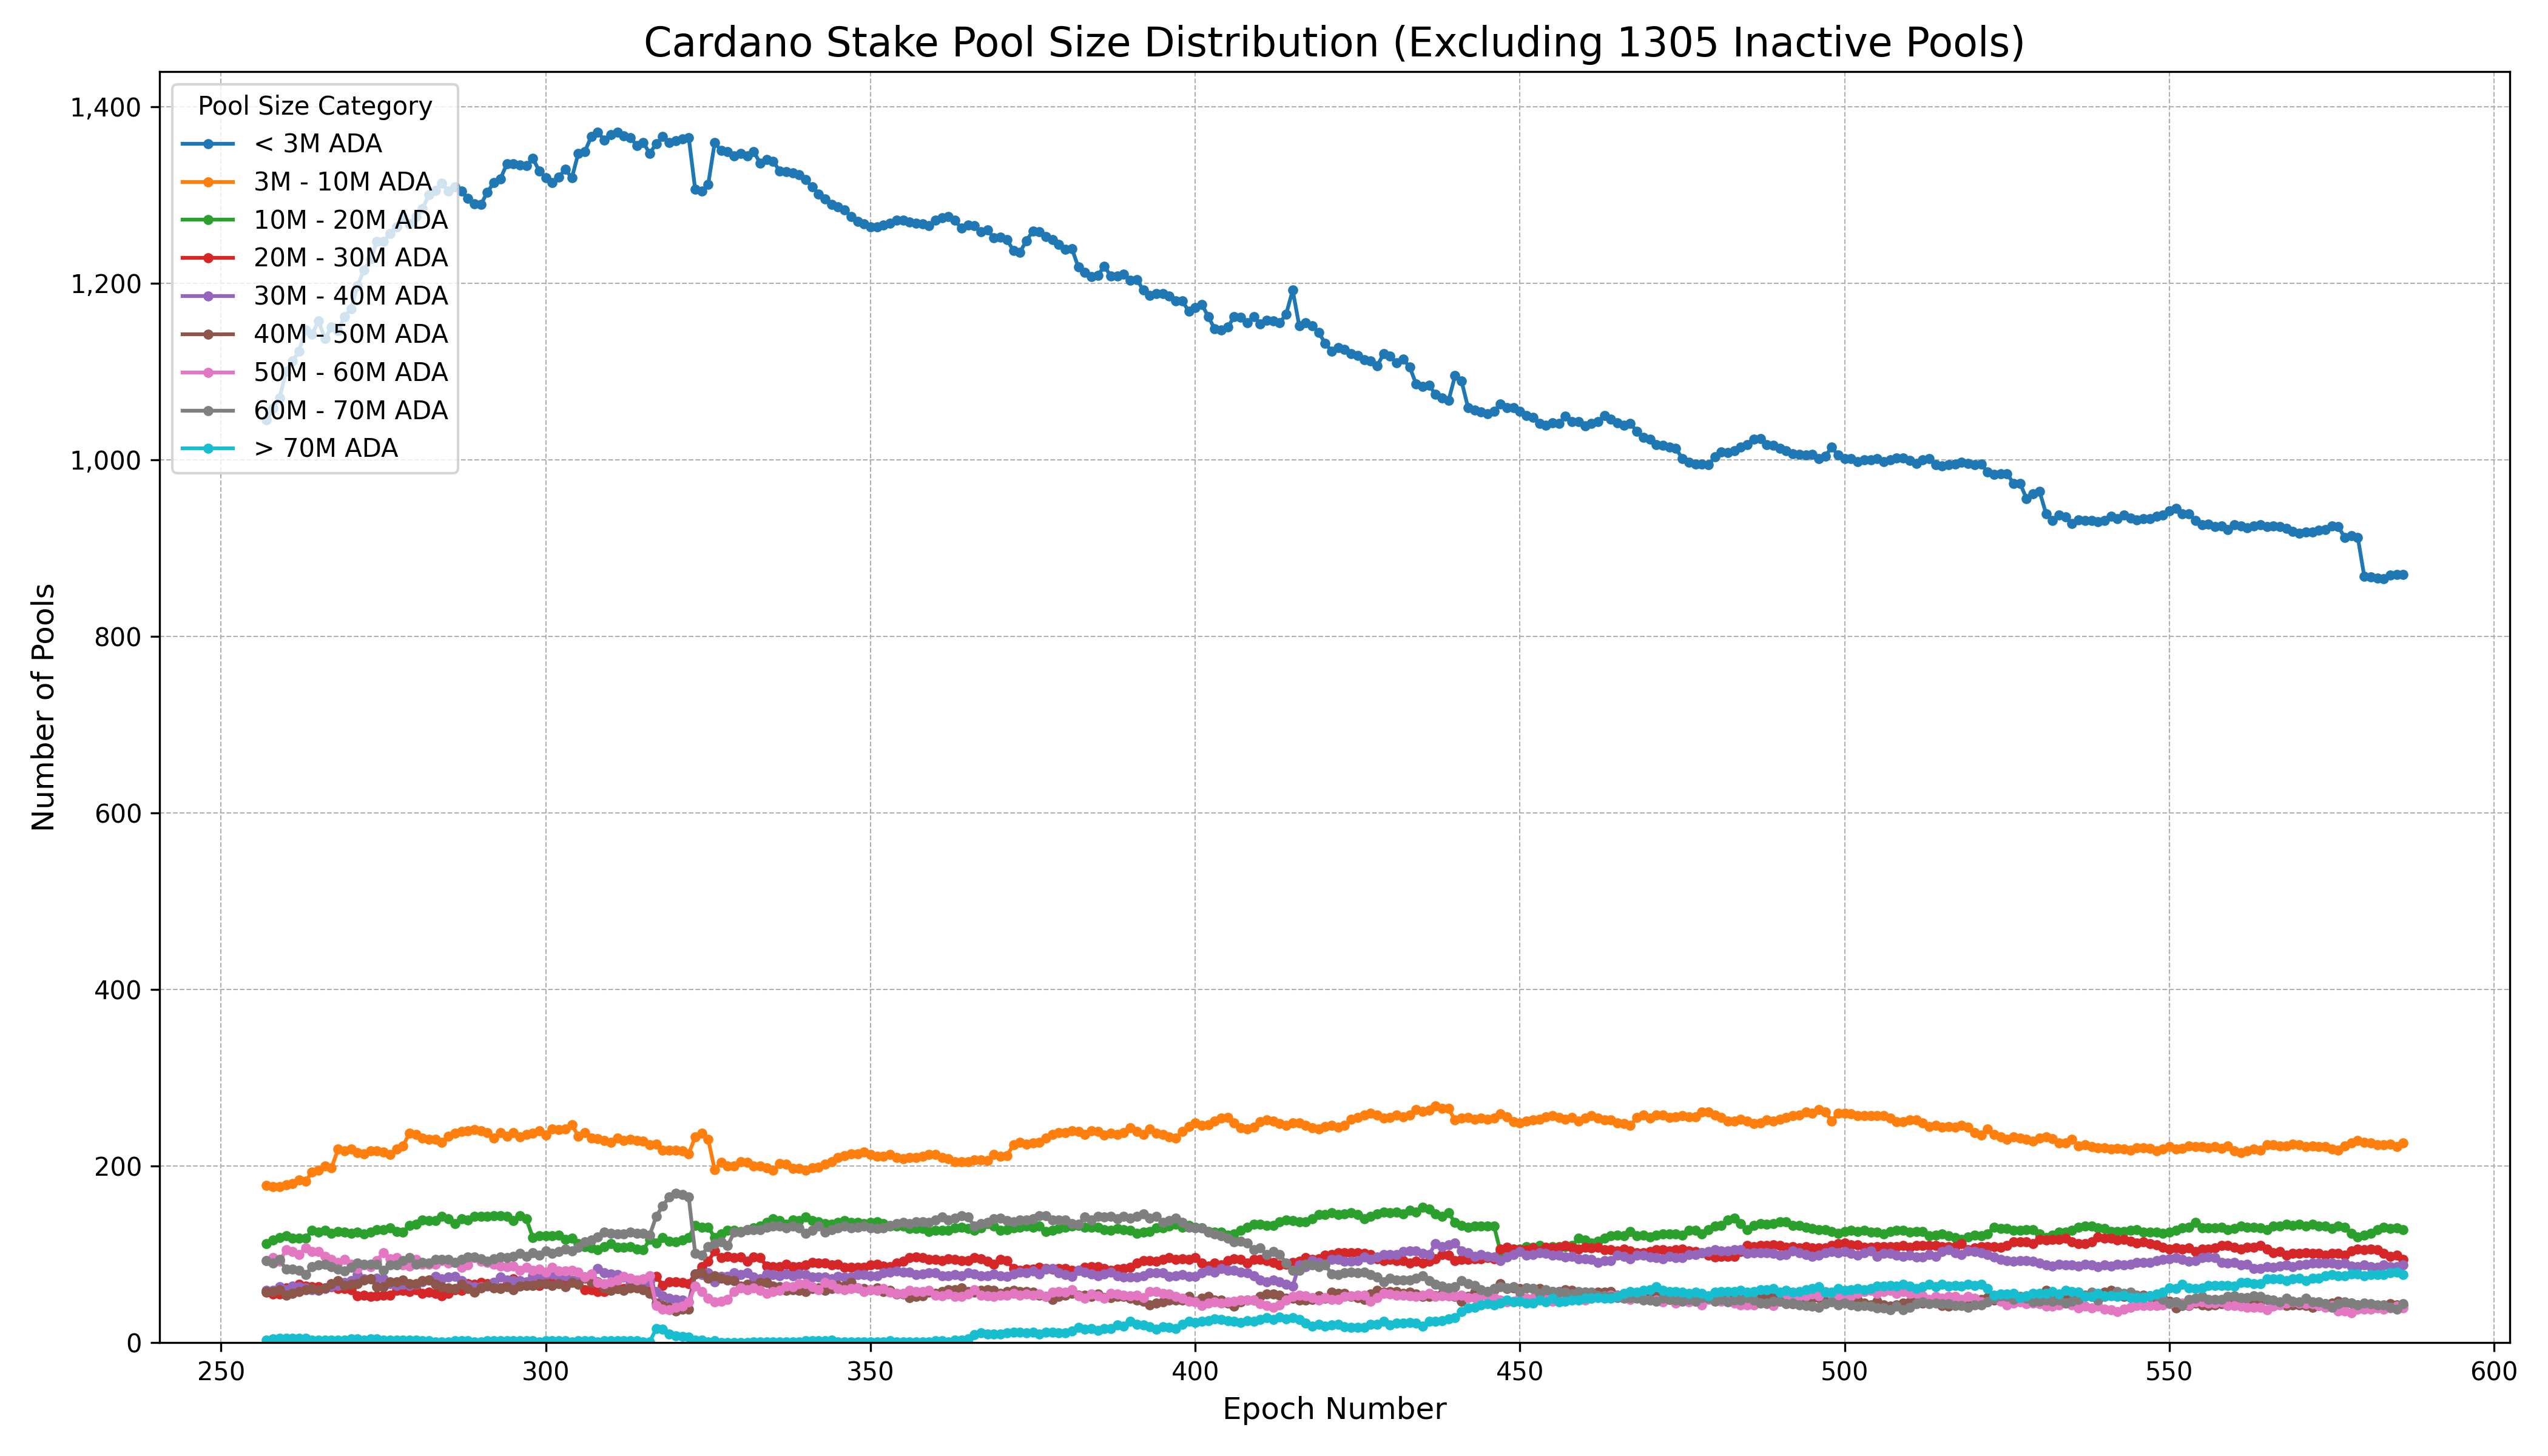
\includegraphics[width=\textwidth]{img/pool_size_distribution.png}
	\caption{Pool size distribution. This chart shows the
		number of active pools within each size category}\label{fig:pool-dist}
\end{figure}

Figure~\ref{fig:stake-control} provides a historical lens on stake allocation
by pool size categories over epochs, excluding the 1,305 abandoned pools. This time-series
data shows steady growth in the upper tiers amid active stake fluctuations. These patterns
are consistent with the game-theoretic design, which predicted delegators would favor larger
pools, leading to a concentrated core of operators. This clustering results in 741 healthy
pools securing the majority of stake.

Key insights from this data include:

\begin{itemize}
	\item \textbf{Robust supply and targeted demand}: The number of smaller pools signals community
	      interest in operating Stake Pools, while the concentration of delegation reflects market
	      behavior consistent with the incentive model’s predictions. As the model predicted, this dynamic
	      directs stake toward high-return pools. This enhances network stability without compromising diversity.
\end{itemize}

\begin{figure}[H]
	\centering
	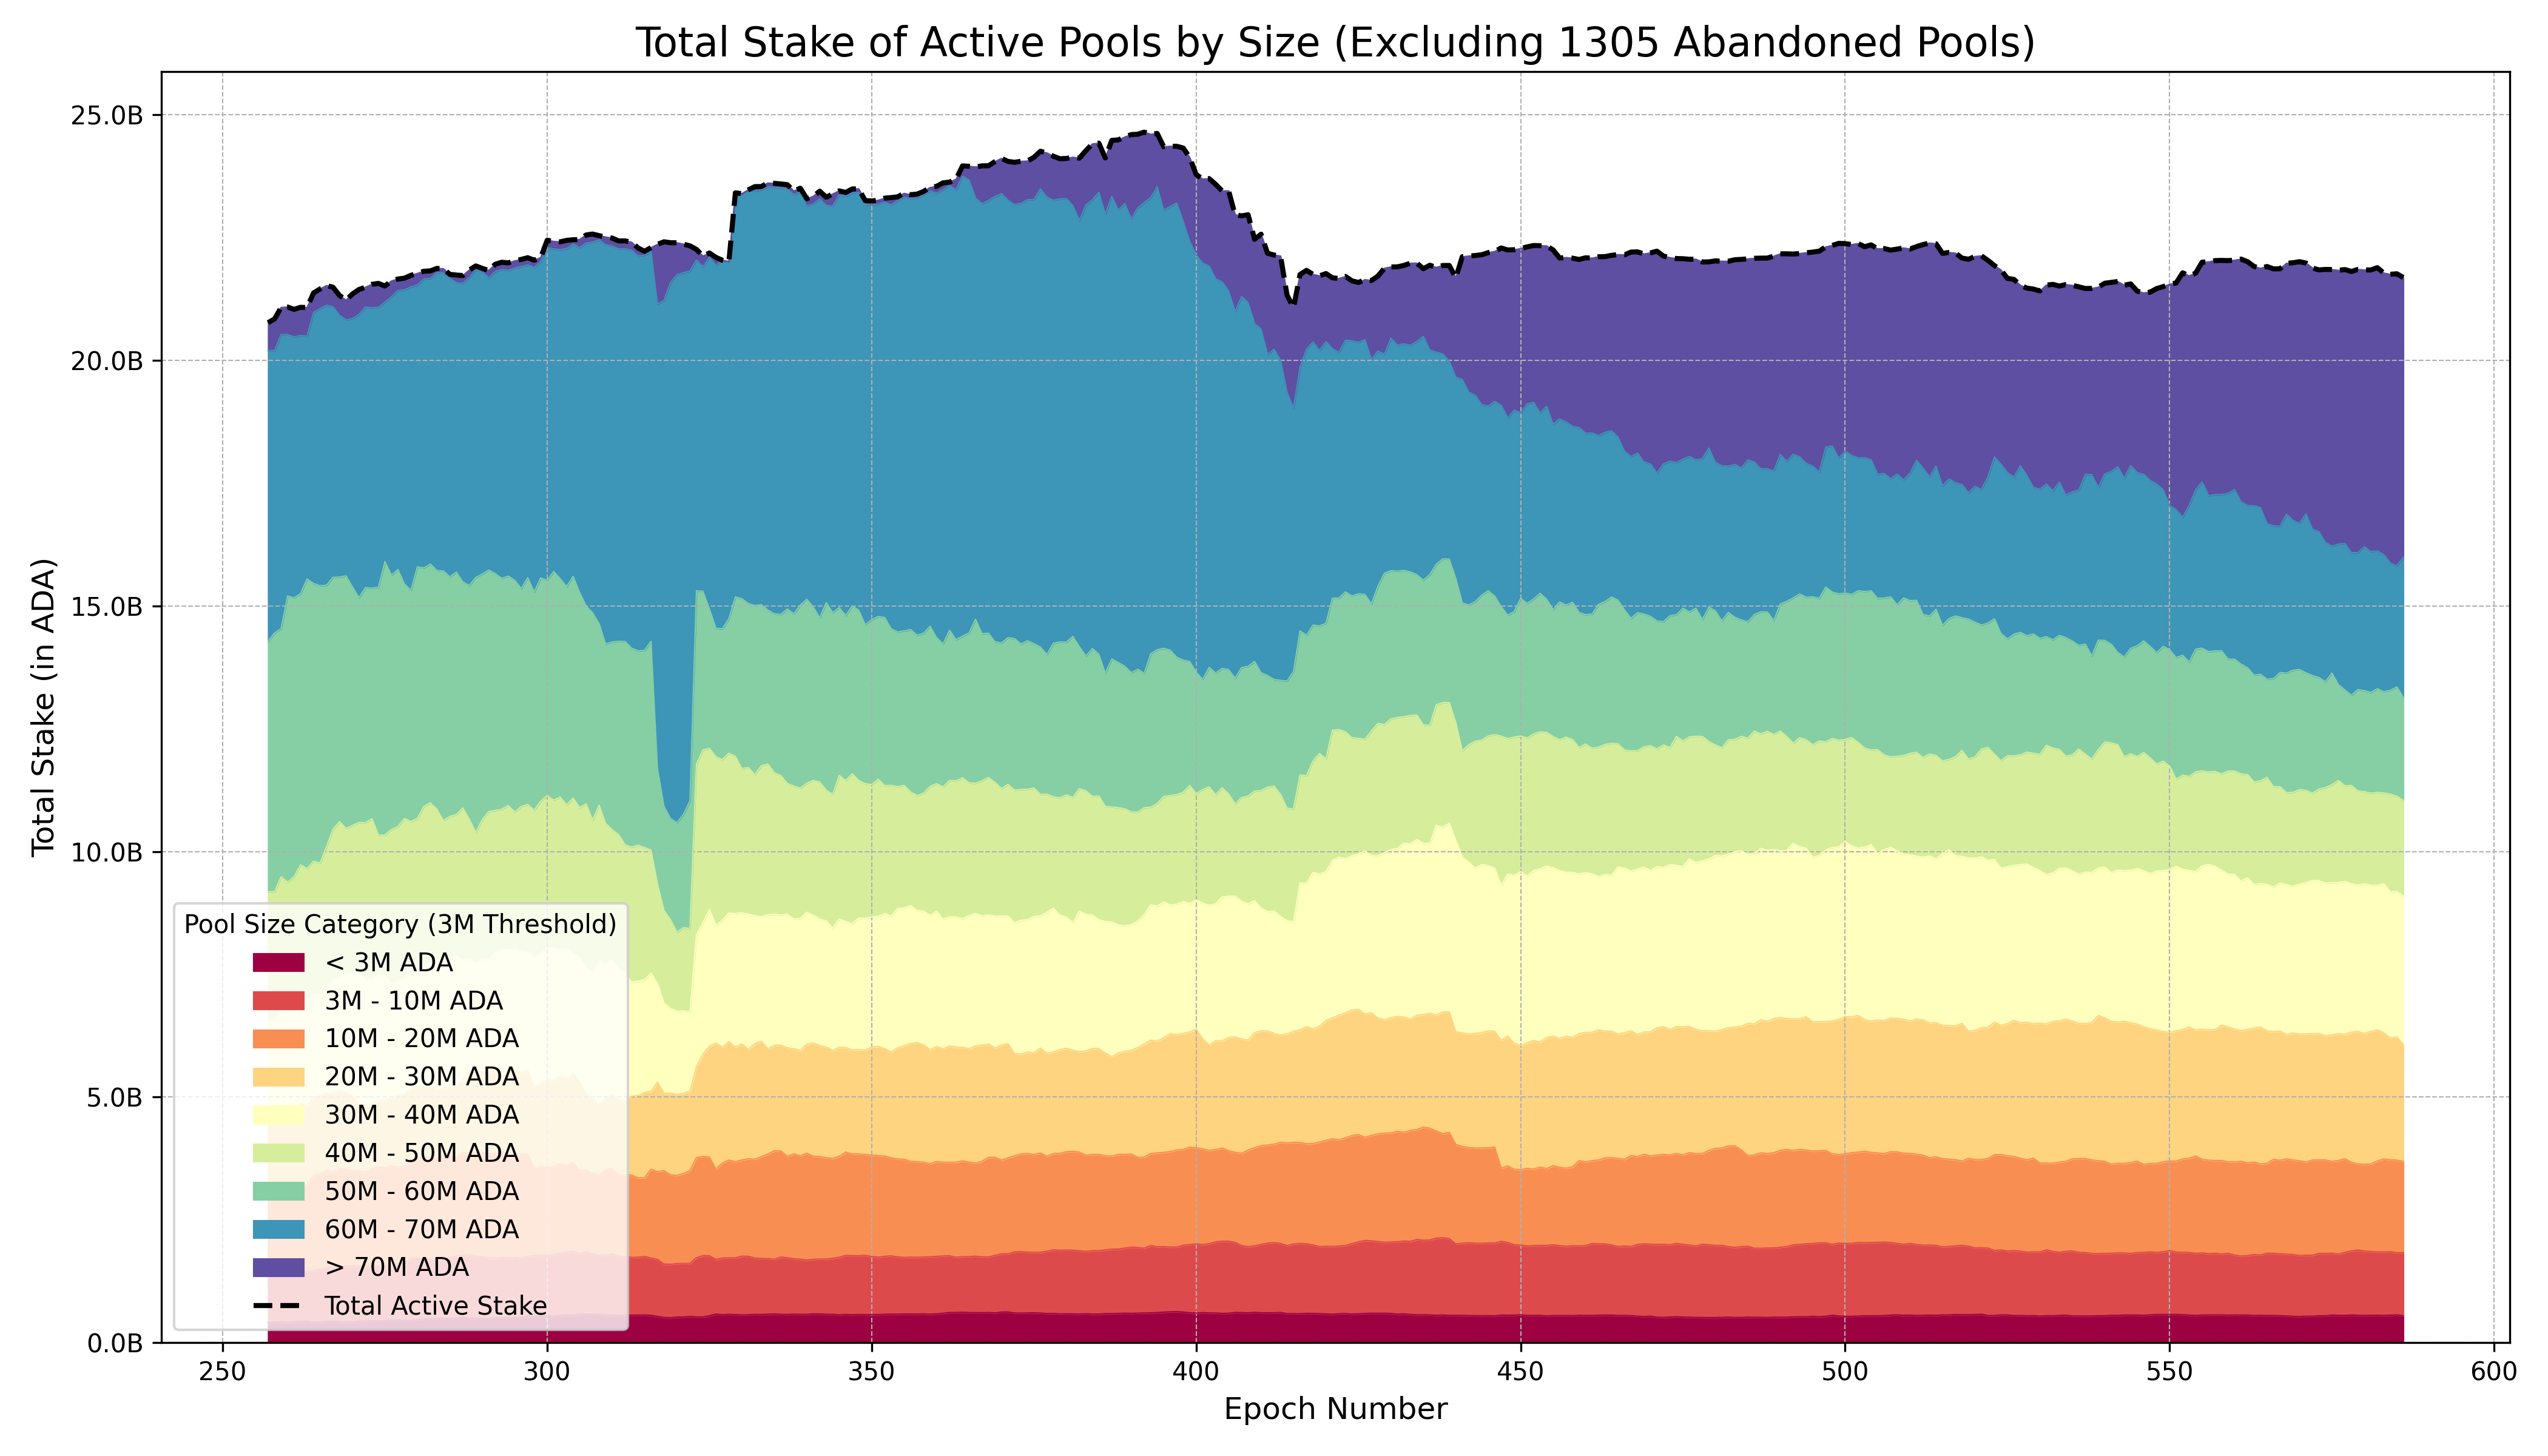
\includegraphics[width=\textwidth]{img/stake_control_by_size.png}
	\caption{Total Stake of Active Pools by Size. This stacked area chart depicts
		the evolution of stake (in billions of ADA) across size categories over epochs,
		alongside the cumulative total active stake (black line).}\label{fig:stake-control}
\end{figure}

\newpage
\subsubsection{Wallet distribution and stake control}

The on-chain distribution of delegated ADA, illustrated in Figure~\ref{fig:wallet-dist}, is highly concentrated. While over one million wallets
hold less than 1,000 ADA, their collective stake is negligible at 0.03\%.
Conversely, a cohort of approximately 4,500 wallets, each holding over 500,000
ADA, controls a significant majority (68.5\%) of the total delegated stake.

This Pareto-like distribution of capital primarily determines the delegation market's dynamics.
The concentration of stake among a small number of large holders creates a significant barrier
to growth for new and smaller pools, as these large-stake entities are rationally incentivized to delegate to
established, high-performance operators or to operate their own private pools.
It must be noted that this analysis is limited to on-chain data and does not account for holdings
on exchanges or in custodial services, suggesting the true concentration of capital may be even more pronounced.

This distribution provides the necessary context for understanding the
competitive environment in which stake pools operate and the structural
challenges they face in attracting delegation.

\begin{figure}[H]
	\centering
	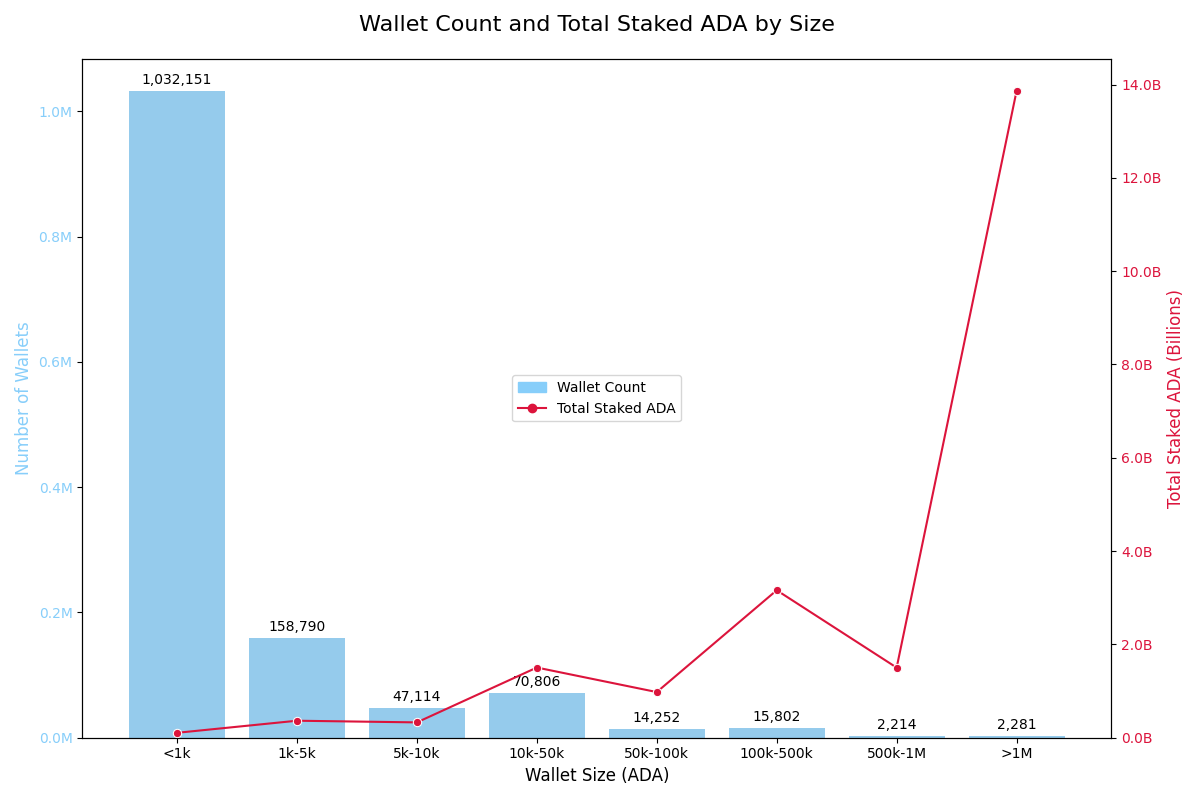
\includegraphics[width=\textwidth]{img/wallet_distribution_combined_corrected.png}
	\caption{Wallet count and total staked ADA by size. This chart illustrates the skewed distribution of
		ADA holdings across network wallets.}\label{fig:wallet-dist}
\end{figure}

\subsection{The four tiers of stake pool viability}

We developed a classification system based on an analysis of all active pools
over the last 36-epoch period (Epochs 548 to 583). The methodology evaluates
each pool's performance against two benchmarks derived from the previous
analysis:

\begin{itemize}
	\item \textbf{Stake threshold of 3 million ADA}, which ensures a 95\% probability of producing at least
	      one block per epoch.
	\item \textbf{Rewards threshold of 5,500 ADA} over the analysis window, which roughly corresponds to the break-even
	      point for covering operational costs of 156 ADA * 36 epochs.
\end{itemize}

In addition to these quantitative measures, pools were assessed for qualitative
signals of inactivity, such as:

\begin{itemize}
	\item Unmet pledge at the end of the analysis period.
	\item No pool updates during the analysis period.
	\item Zero block production during the analysis period.
	\item No participation in governance (Delegation or Direct voting) during the
	      analysis period.
\end{itemize}

By combining these financial and operational indicators, each pool was assigned
to one of the four viability tiers.

\begin{table}[H]
	\centering
	\begin{tabularx}{\textwidth}{@{}l X rr@{}}
		\toprule
		\textbf{Status}               & \textbf{Description}                                      & \textbf{\makecell[r]{Number                    \\ of Pools}} & \textbf{\makecell[r]{Controlled \\ Stake (ADA)}} \\ \midrule
		\textbf{Inactive}             & Unmet Pledge plus another sign of neglect and no blocks   & 1305                        & 46.87 M          \\
		\textbf{Active \& Struggling} & $<$ 3M Stake \& $<$ 5500 ADA in cumulative rewards        & 627                         & 190.83 M         \\
		\textbf{Active \& Viable}     & Viable but small ($<$ 3M ADA stake, $>$ 5500 ADA rewards) & 246                         & 368.07 M         \\
		\textbf{Healthy}              & Healthy ($>=$ 3M ADA stake)                               & 741                         & 21.14 B          \\ \midrule
		\textbf{Total Active}         &                                                           & \textbf{1614}               & \textbf{21.70 B} \\
		\textbf{Grand Total}          & All Non-Retired Pools                                     & \textbf{2919}               & \textbf{21.74 B} \\ \bottomrule
	\end{tabularx}
	\caption{Summary of all registered pools by viability status for epochs 548--583.
		\textit{[Appendix A (appendixA.txt) contains a comprehensive report on all non-retired pools by viability status.]}}
	\label{tab:viability-summary}
\end{table}

\paragraph{The inactive layer:} The largest group, comprising 1,305 pools, is
classified as \texttt{Inactive}. These operators have failed to meet viability thresholds and show multiple
signs of abandonment. While this is a large number of pools, their economic
impact is negligible. Together, they control only \textasciitilde47 million
ADA, less than 0.22\% of the delegated stake. This ``long tail'' of inactive
pools does not pose a systemic risk to the network's security.

\paragraph{The active ecosystem: healthy, viable, and struggling pools:} The competitive landscape is made up of 1,614 pools classified as
\texttt{Active}. These operators are actively maintaining their infrastructure
and competing for delegation. This active group is not monolithic and can be
broken down into three sub-categories.
\begin{itemize}
	\item \textbf{Healthy (741 Pools):} This is the core of the Cardano network. These operators have surpassed
	      the 3M ADA viability line, ensuring consistent block production and financial sustainability. They control
	      the majority of the network's stake (21.14 billion ADA) and are responsible for most of its security and
	      block production. The existence of a large and diverse set of healthy operators is an indicator of the
	      incentive scheme's success.
	\item \textbf{Viable but small (246 Pools):} This is a group of operators who have not yet reached the 3M
	      ADA stake threshold but have demonstrated strong performance by earning enough rewards to cover their
	      costs. They control approximately 368 million ADA\@. These pools represent a combination of operational
	      skill, community support, and statistical luck.
	\item \textbf{Struggling (627 Pools):} This large group of operators is actively participating but failing
	      to achieve financial viability. They have neither the stake for consistent block production nor the cumulative
	      rewards over the analysis period to cover their costs. Collectively control about 191 million ADA\@. Their long-term
	      sustainability is uncertain.
\end{itemize}

The large number of pools in the \texttt{Viable but Small} and
\texttt{Struggling} categories (873 total) points to a large portion of the
operator community facing challenges with scale.

This suggests the potential benefit of an on-chain mechanism that would allow
them to form alliances. Such a mechanism could enable thesegroups to combine
resources and operational duties, creating a larger, more reliable, and
cost-efficient `virtual stake pool'. This capability is, of course, very common
in the traditional markets, companies form consortia, joint ventures, and
strategic alliances to pool resources and share risks. We think this is an
interesting avenue for future research for Cardano.

\subsection{System in equilibrium}

\subsubsection{Network's state over a 36-epoch period}

An empirical analysis of the network's state over the last 36-epoch period (Epoch 548
to 583) reveals a system that has settled into a multi-faceted and stable
equilibrium. The core indicators of network health, overall stake participation
and block production efficiency, demonstrate a consistent operational
state, as shown in Figure~\ref{fig:macro_stability}.

\begin{figure}[H]
	\centering
	\begin{subfigure}{0.48\textwidth}
		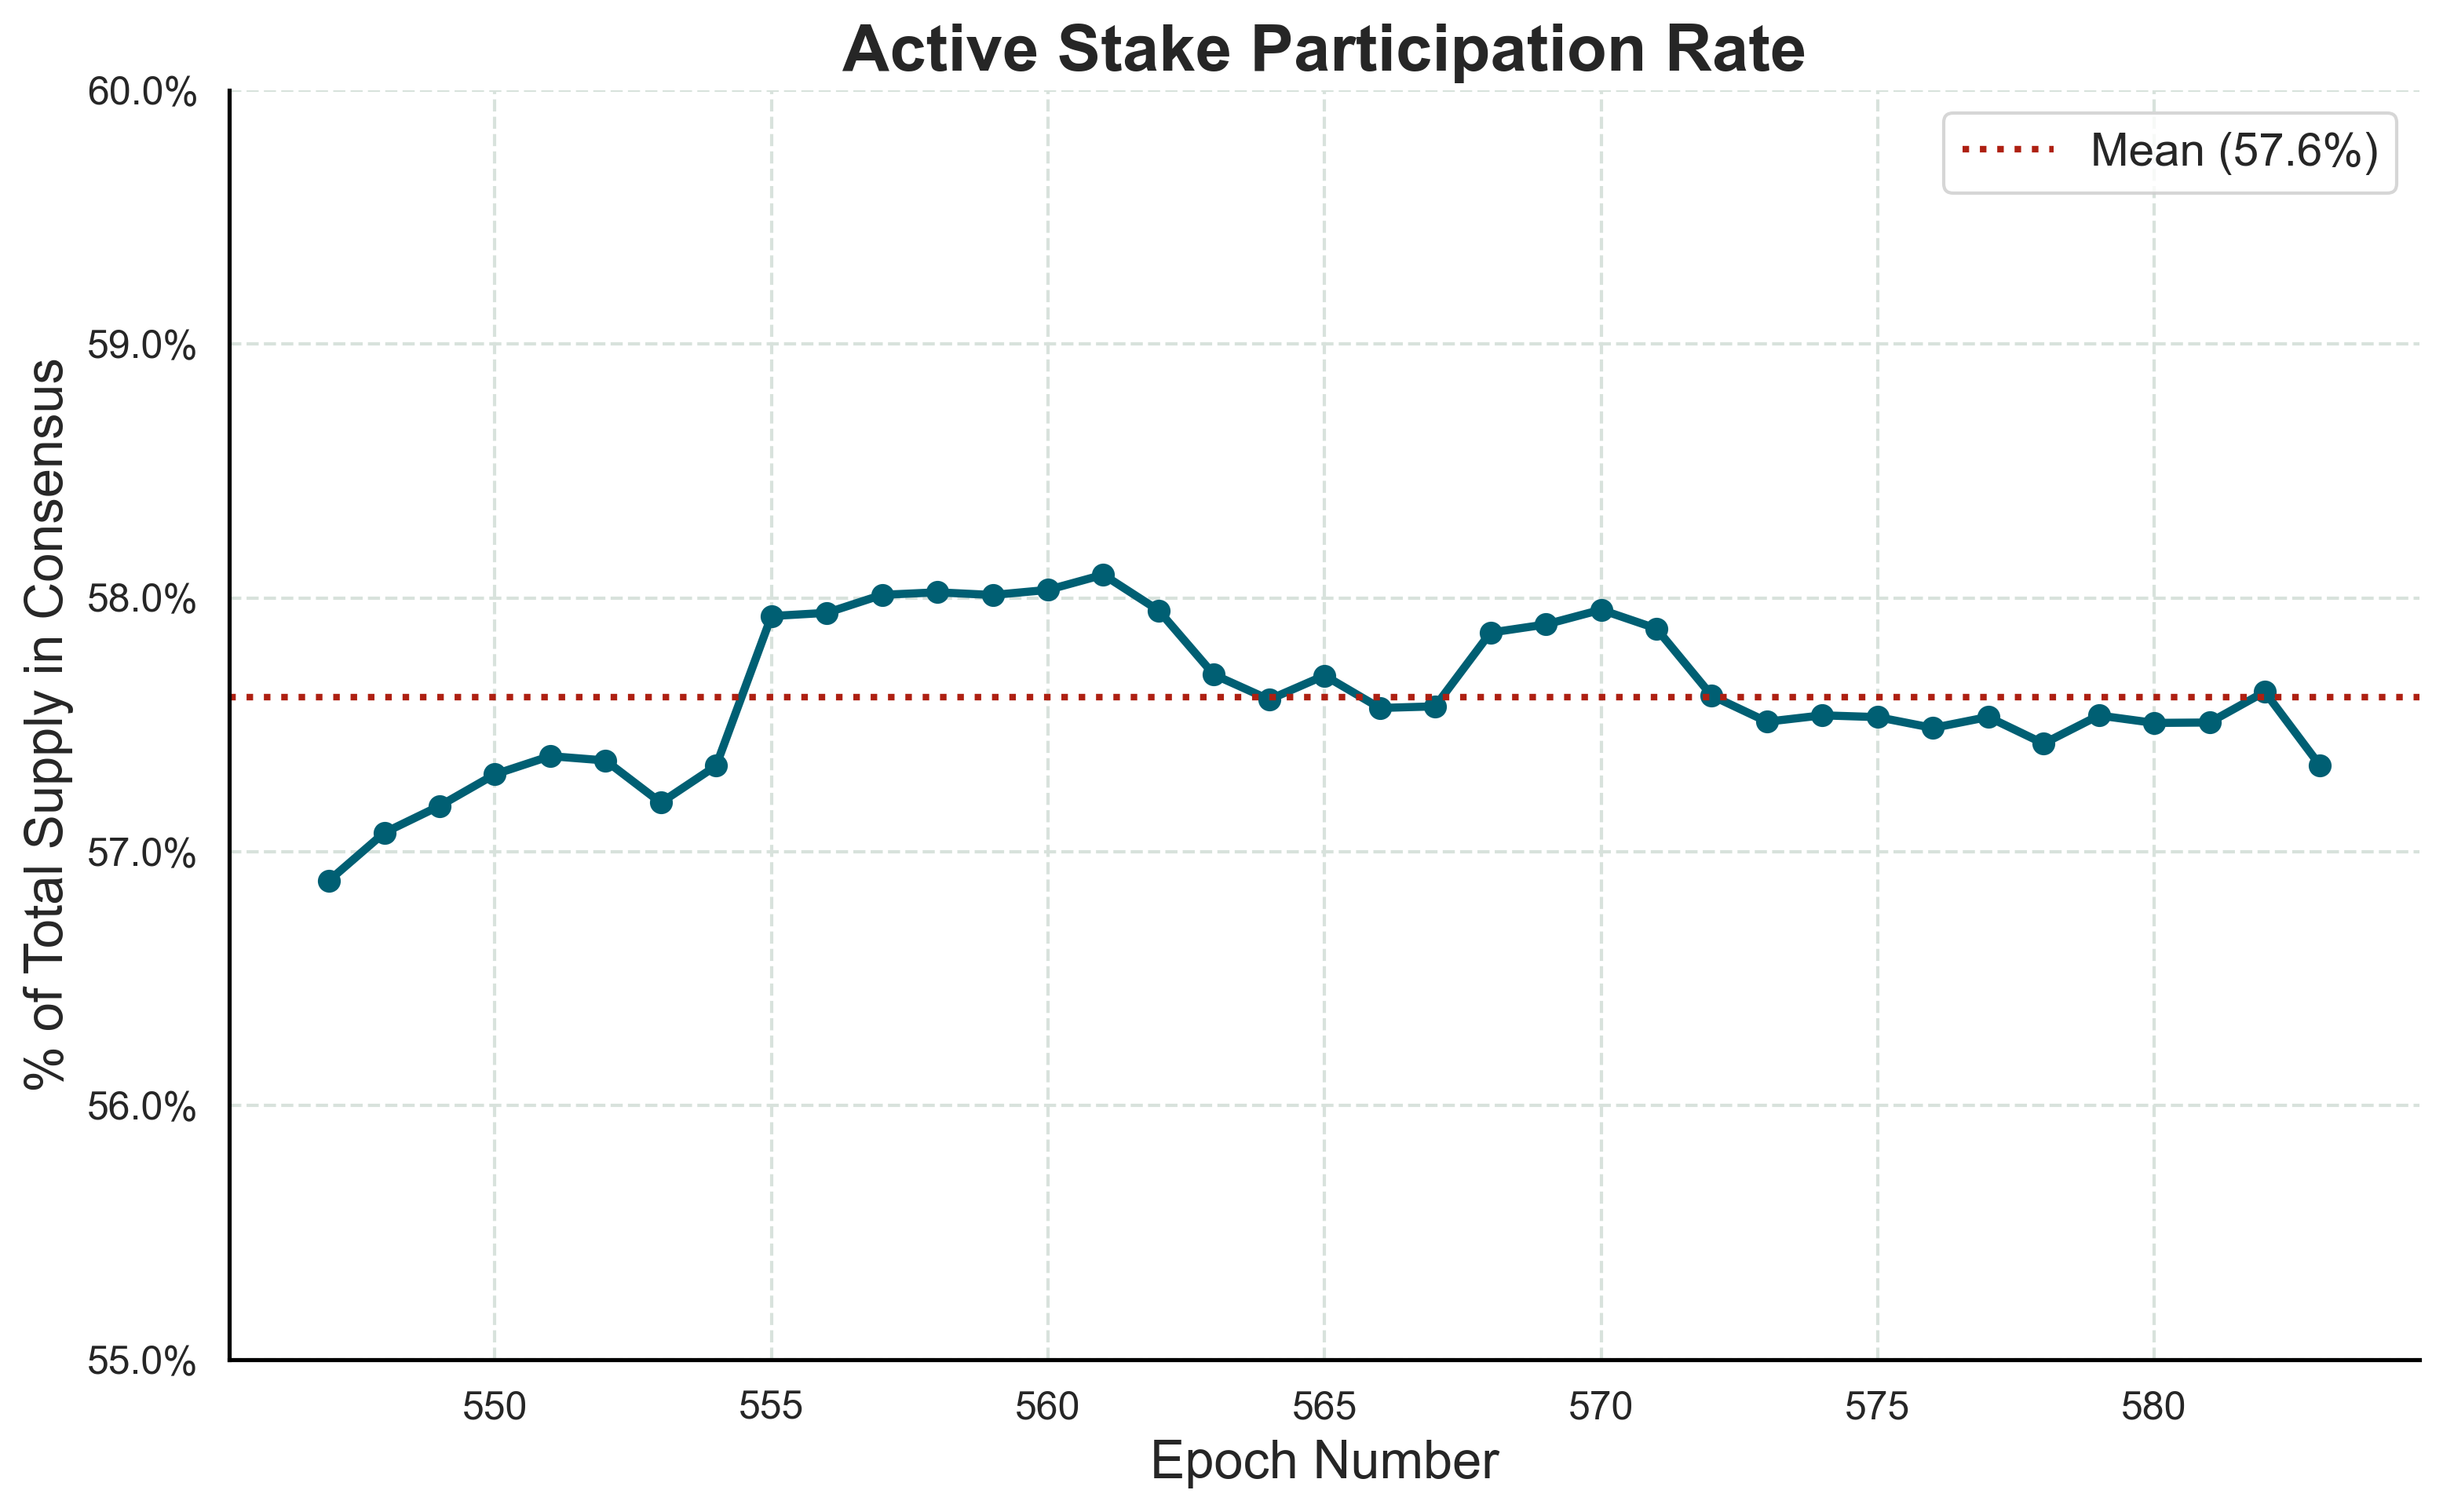
\includegraphics[width=\textwidth]{img/active_stake_participation.png}
		\caption{The percentage of the total circulating supply participating in 
        consensus has remained stable, holding consistently around a mean of 57.4\%.}\label{fig:stake_participation}
	\end{subfigure}
	\hfill % a little space between the figures
	\begin{subfigure}{0.48\textwidth}
		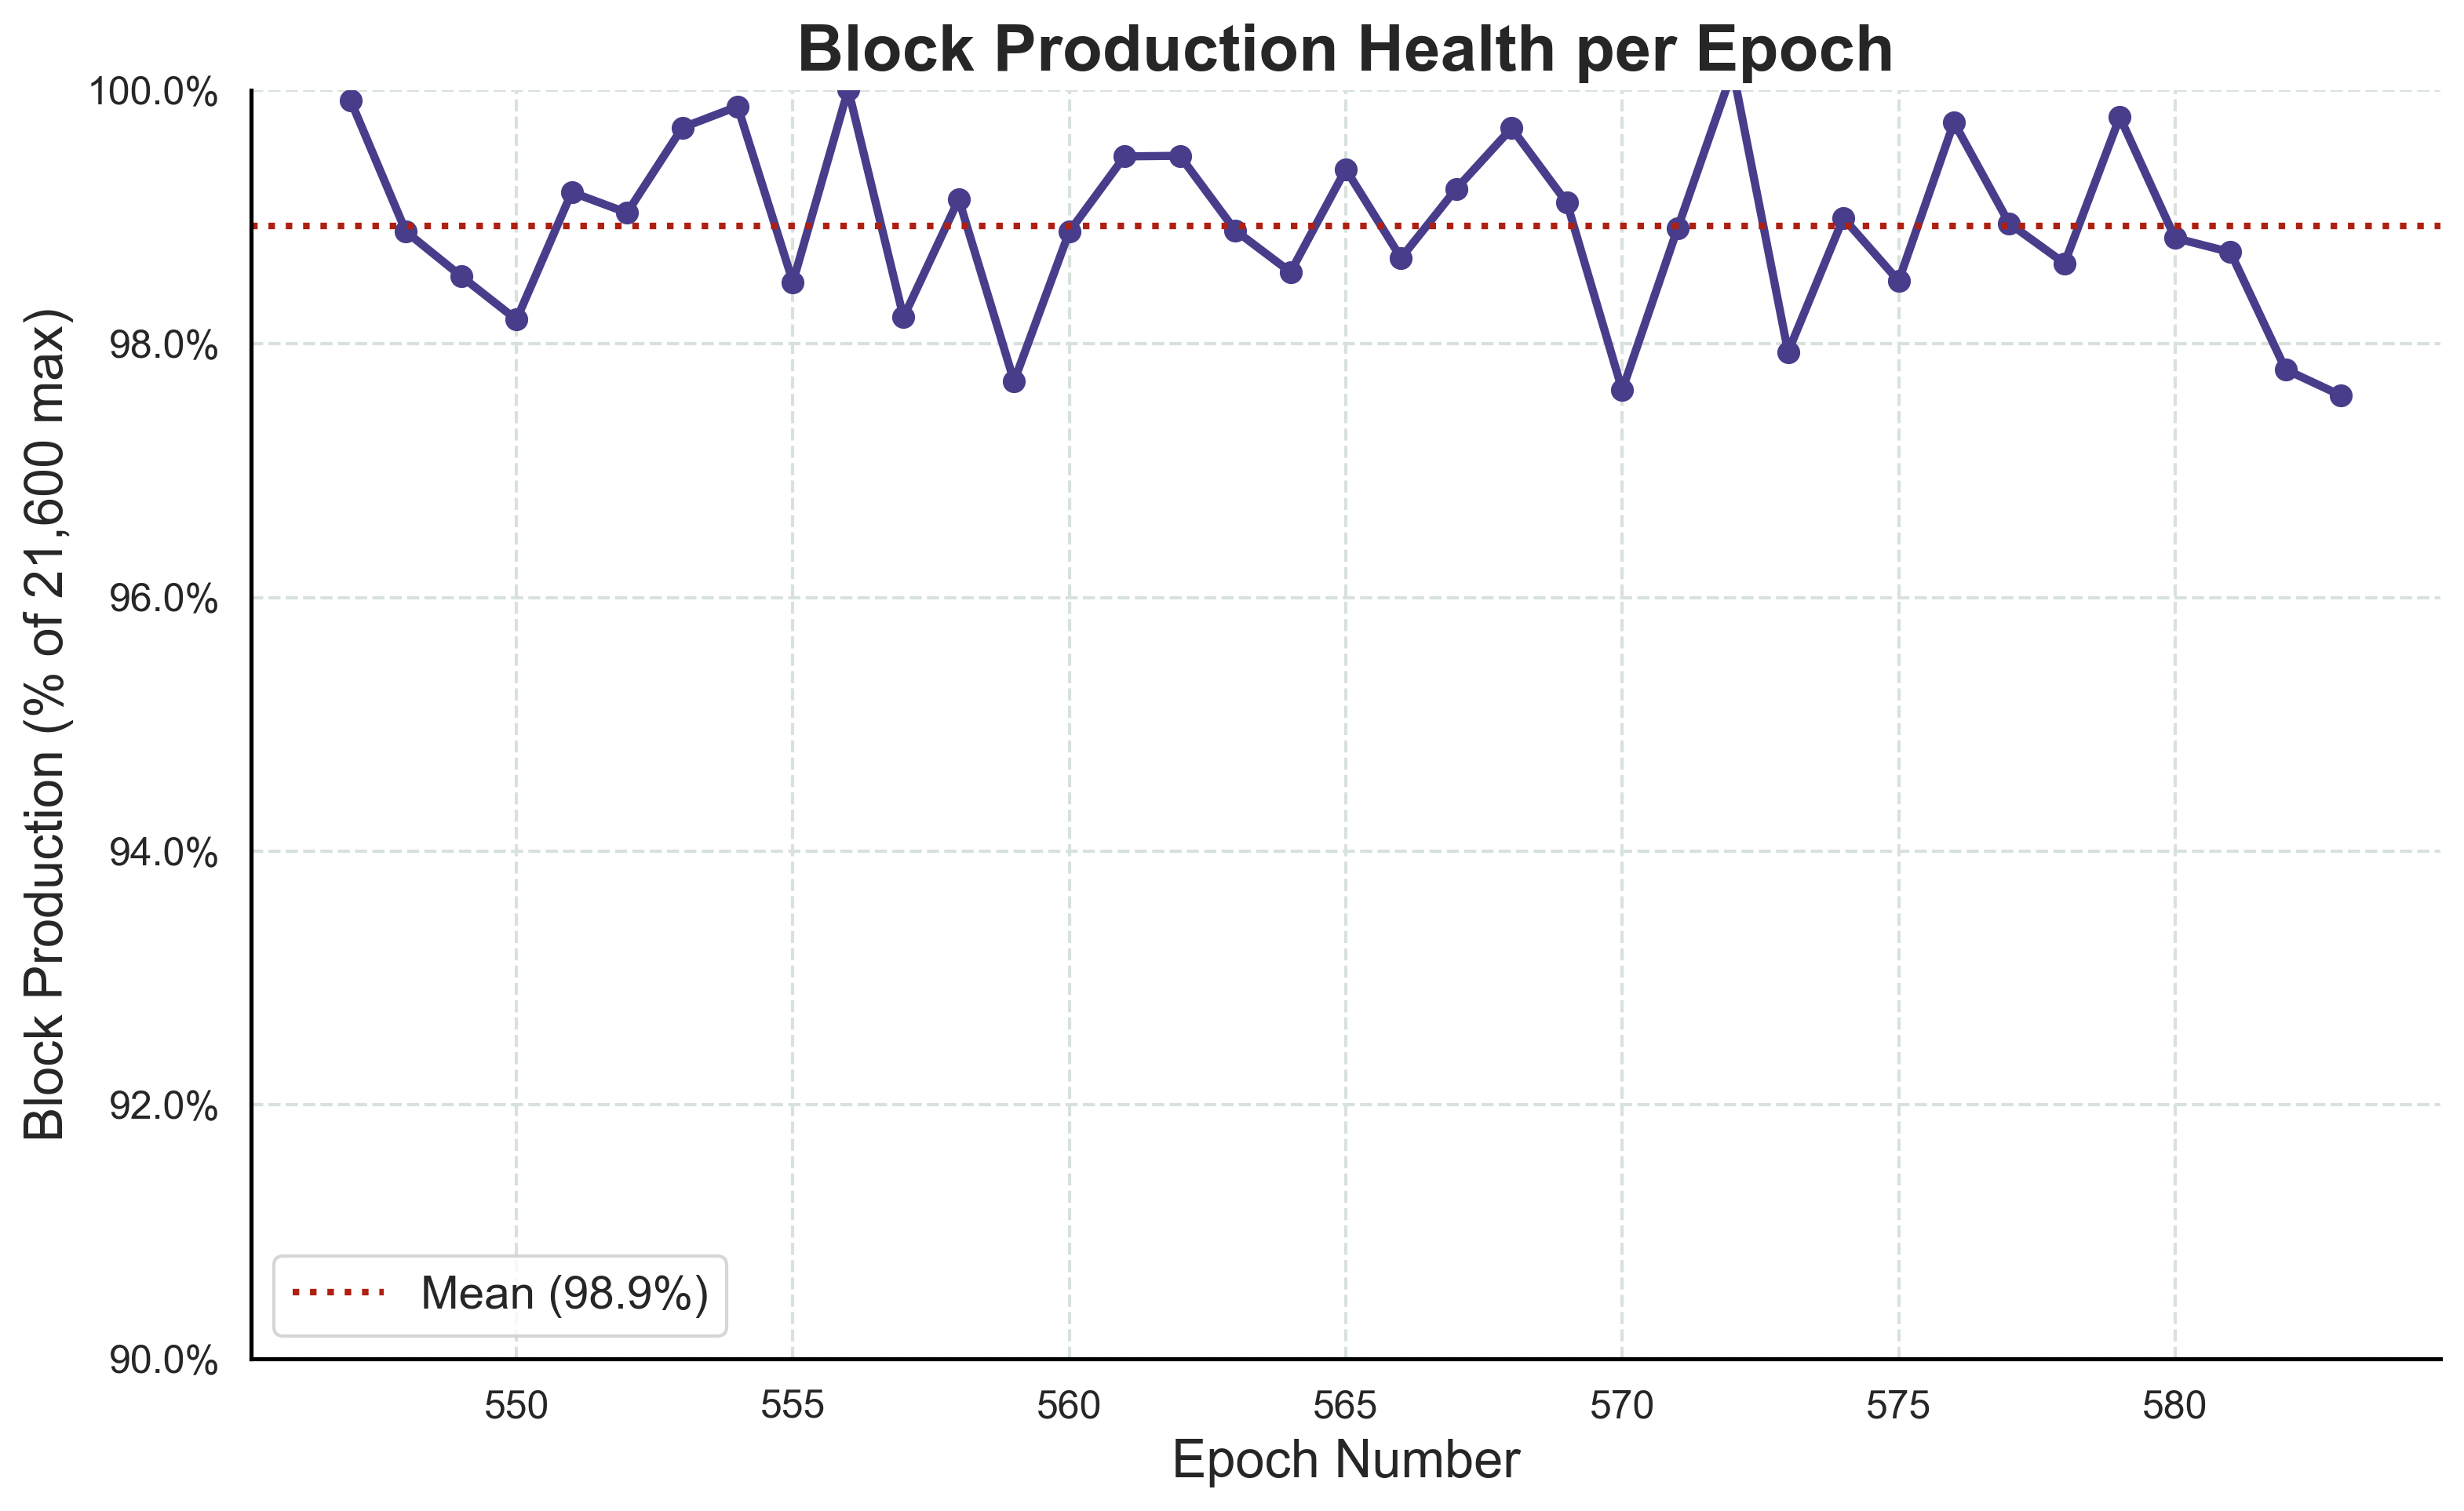
\includegraphics[width=\textwidth]{img/block_production_health.png}
		\caption{Network block production has been highly efficient and reliable, consistently 
        achieving over 95\% of the theoretical maximum of 21,600blocks per epoch.}\label{fig:block_health}
	\end{subfigure}
	\caption{Macro-level indicators of network stability from Epoch 548 to 583.}
	\label{fig:macro_stability}
\end{figure}

This high-level stability is underpinned by a predictable and decentralized
structure of network operators. As illustrated in Figure
\ref{fig:pool_structure}, the system consistently supports over 1,000 unique
pools producing blocks each epoch. Of these, a core group of approximately 741
``Healthy Pools'' (those with active stake exceeding 3M ADA) forms the reliable
foundation of the network. The incentive mechanism has proven highly effective
at concentrating the majority of delegated stake within this group, which
consistently secures over 97\% of all active stake.

\begin{figure}[H]
	\centering
	\begin{subfigure}{0.48\textwidth}
		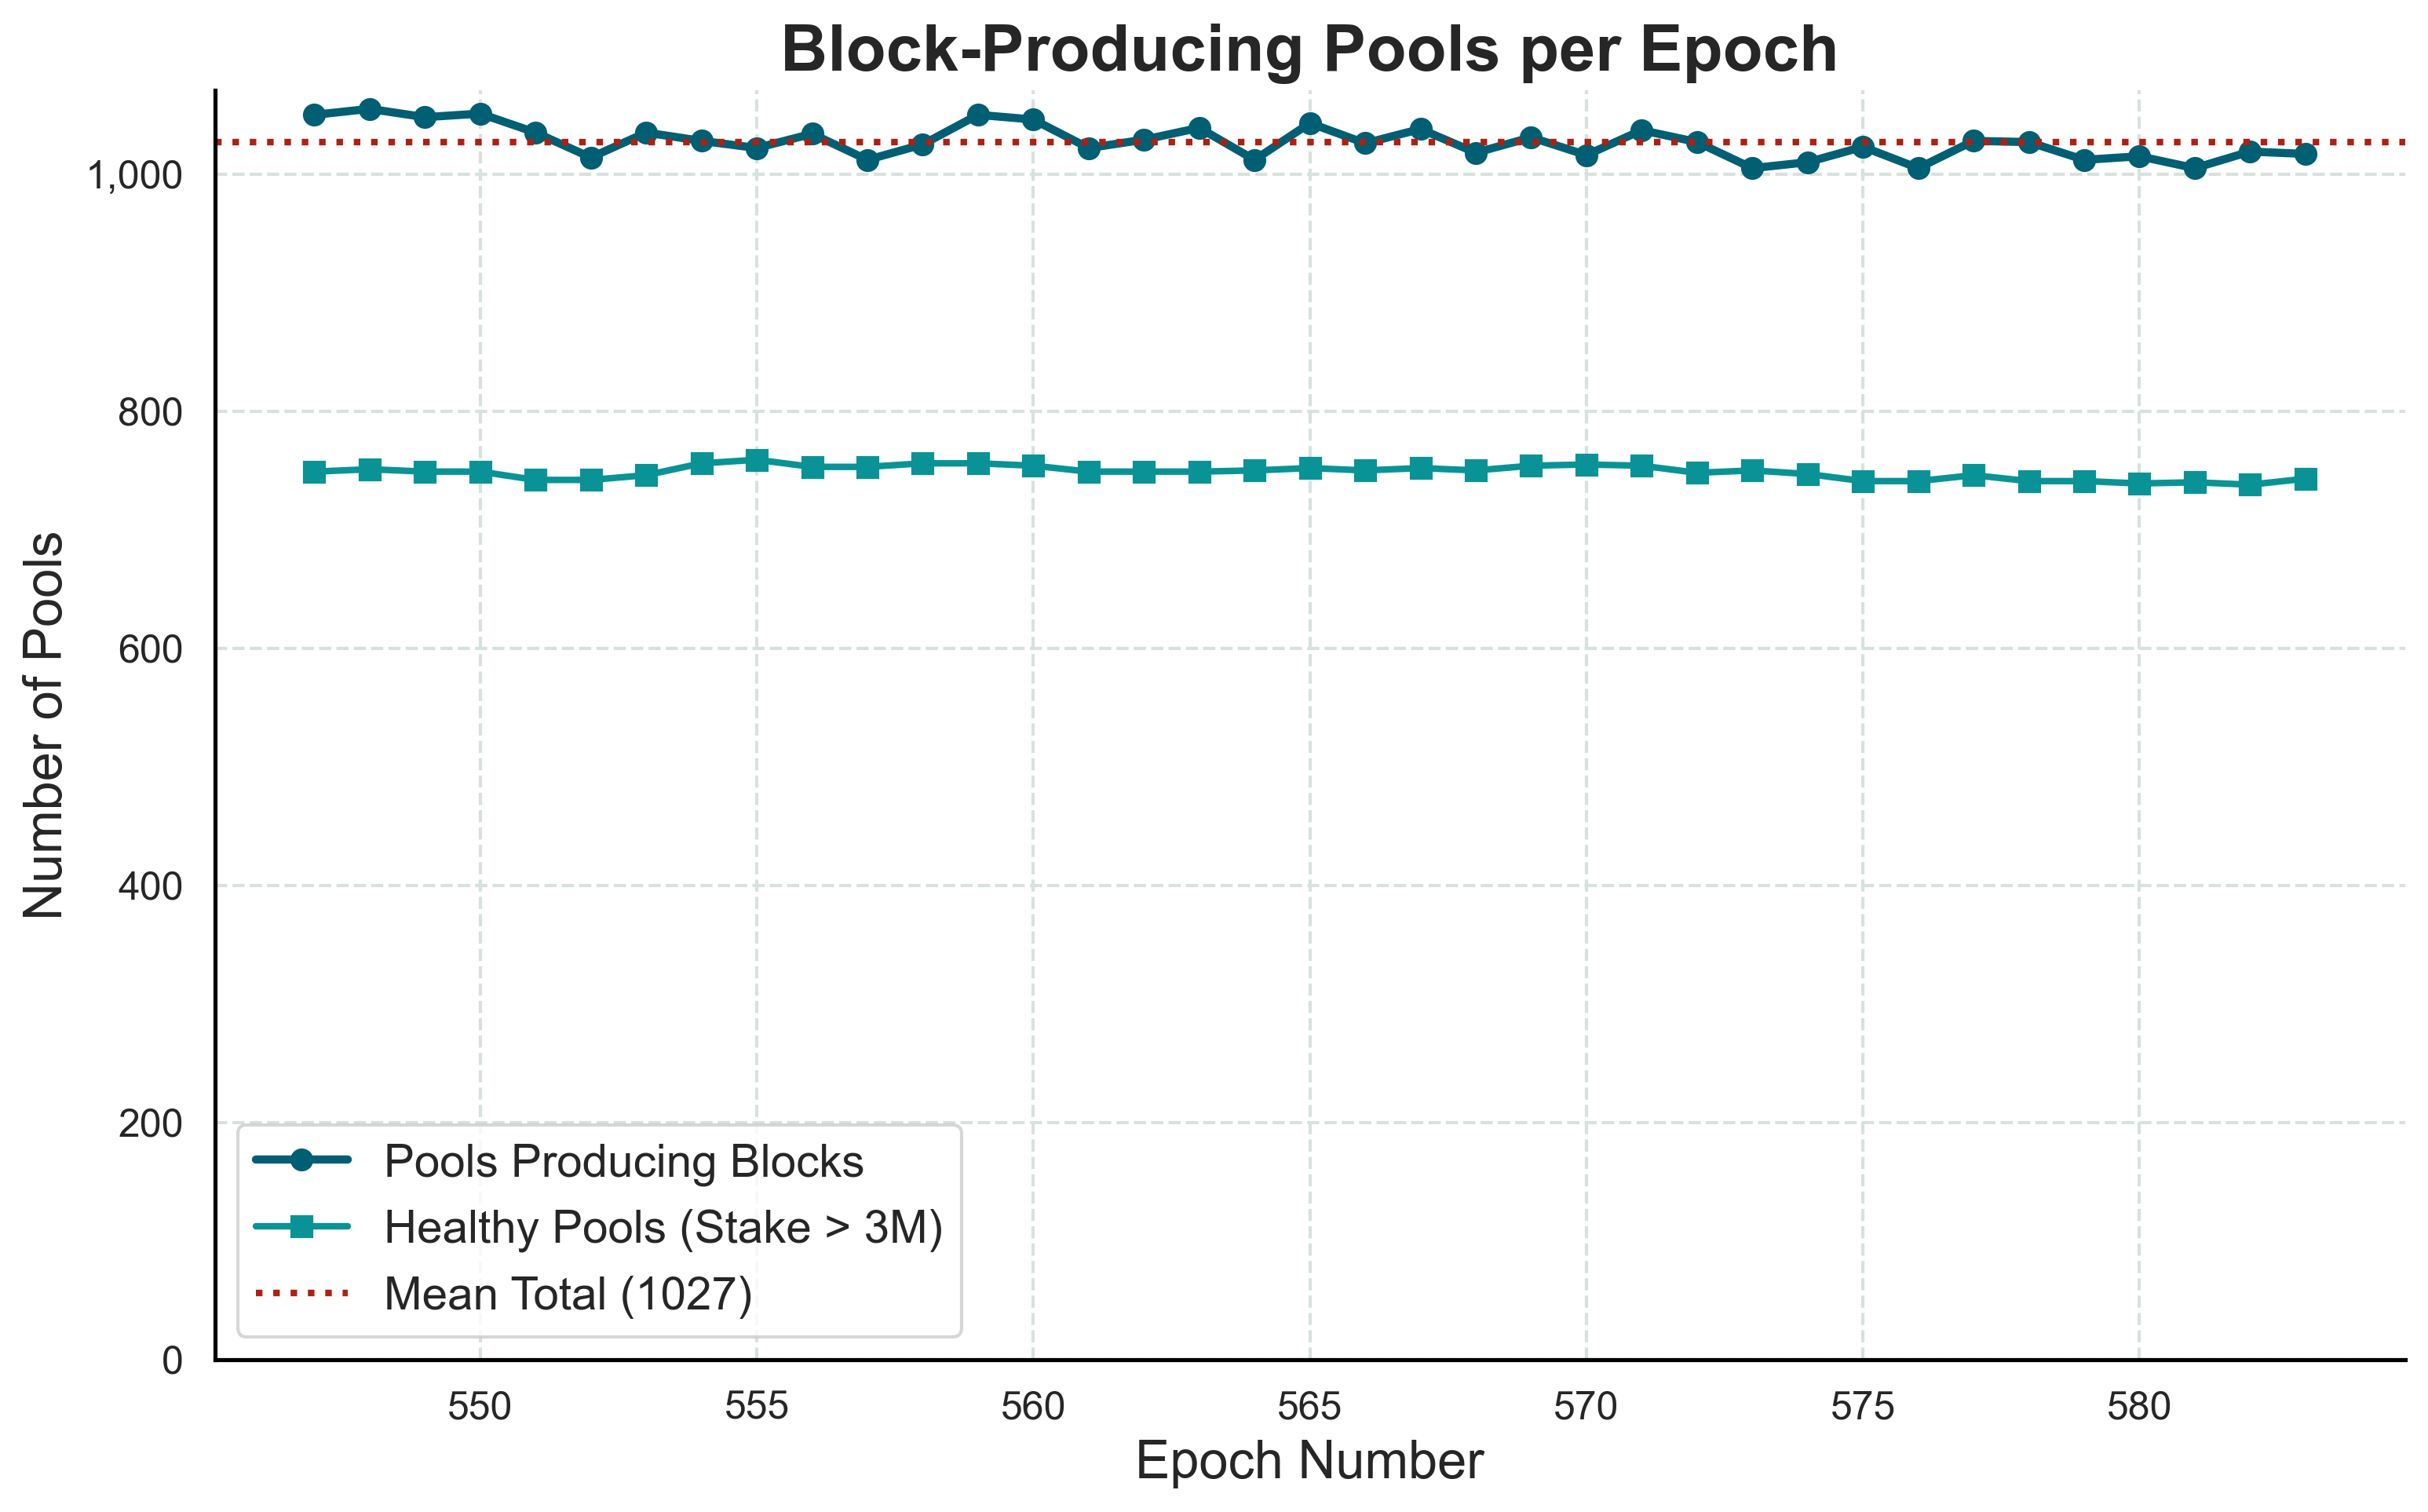
\includegraphics[width=\textwidth]{img/pool_count_epoch.png}
		\caption{The number of pools producing blocks per epoch is highly stable, anchored by a consistent core of Healthy Pools.}
		\label{fig:pool_count}
	\end{subfigure}
	\hfill
	\begin{subfigure}{0.48\textwidth}
		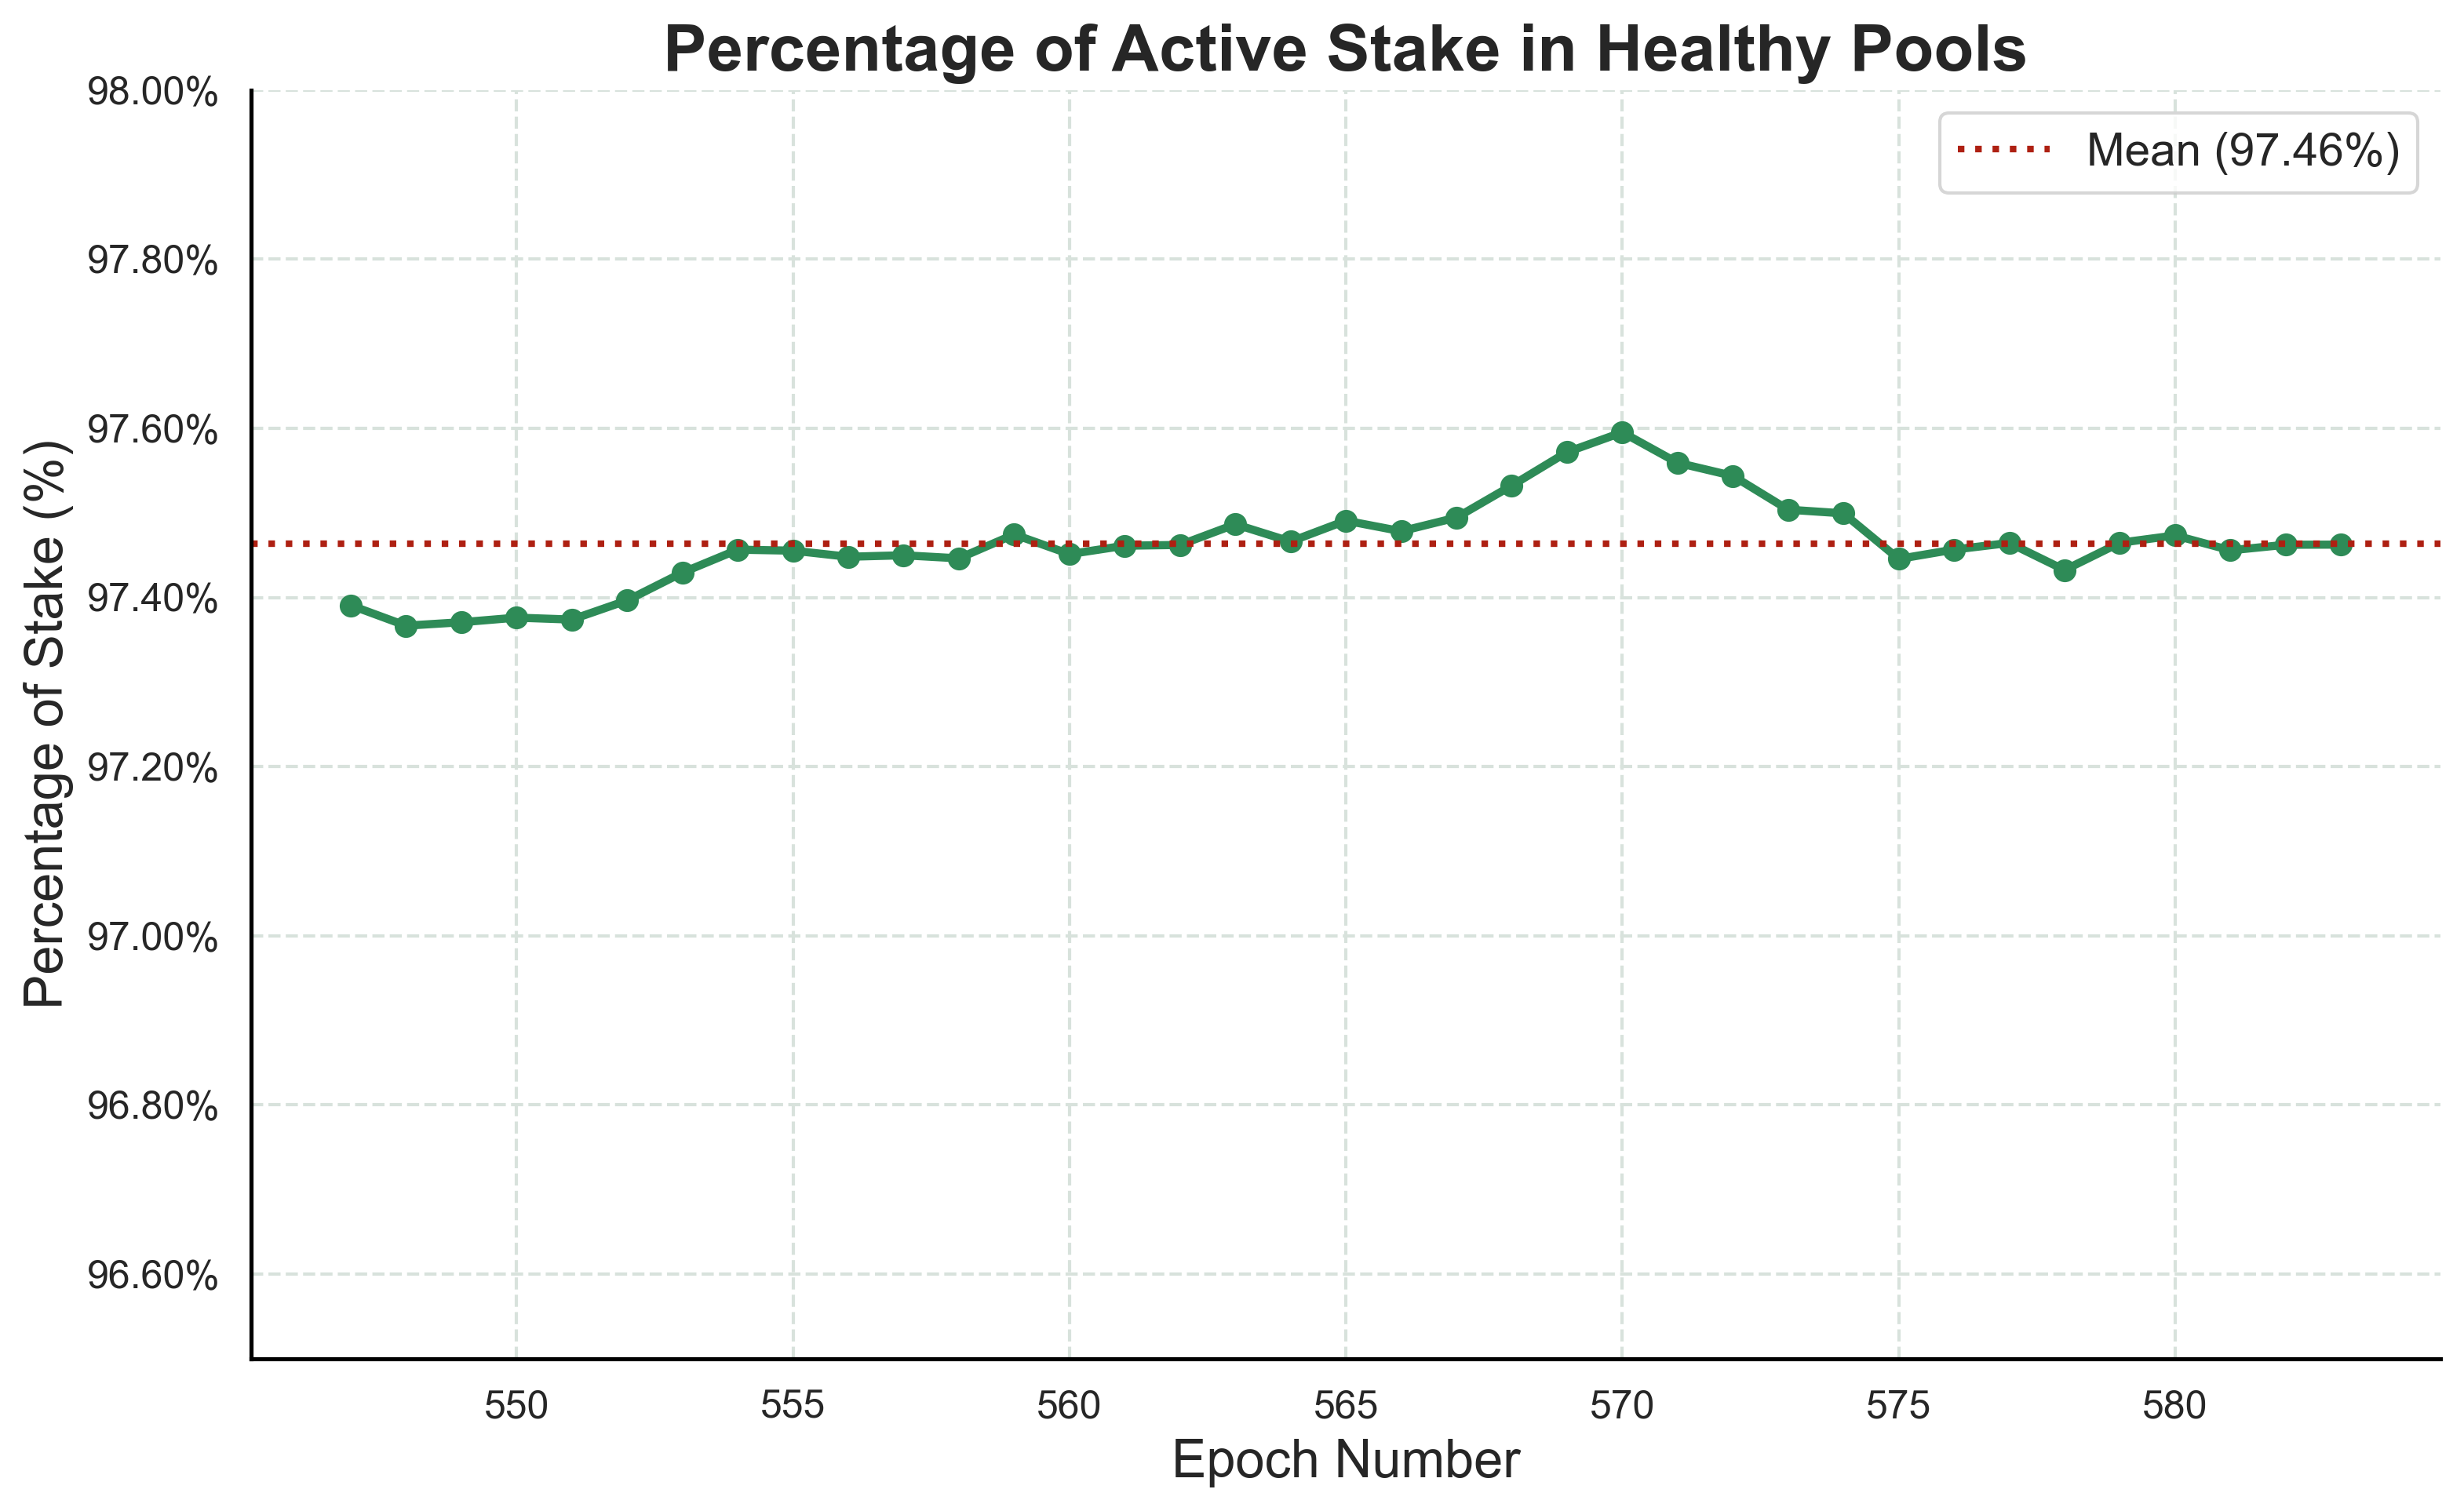
\includegraphics[width=\textwidth]{img/stake_percentage_epoch.png}
		\caption{The percentage of active stake controlled by the Healthy Pools remains constant at over 97\%, confirming a stable delegation equilibrium.}
		\label{fig:stake_percentage}
	\end{subfigure}
	\caption{Distribution and stake control of network operators.}
	\label{fig:pool_structure}
\end{figure}

This stability extends beyond the total stake to the underlying structure of
its distribution. Over the 36-epoch window, the allocation of capital across
pools of different sizes has remained structurally consistent, characterized by
a core of large, healthy pools and a persistent periphery of smaller operators.
For instance, in epoch 548, pools with less than 3M ADA controlled 2.63\% of
the total active stake. By epoch 583, this figure remained nearly unchanged at
2.53\%. In contrast, the largest pools (controlling \texttt{>70M ADA}) saw
their share of stake grow steadily from 19.30\% to 26.26\% over the same
period, indicating a slow but predictable consolidation of capital at the top.
This consistent structure, with its stable periphery and slowly consolidating
core, confirms that the network is not in a state of flux but has reached a
mature equilibrium.

\subsubsection{The impact of stake not participating in consensus}

This observed equilibrium is mathematically constrained. Approximately 16B ADA in circulating supply remains
outside the delegation system, creating a capital-constrained environment that
has shaped the competitive landscape into its current form. See Figure
\ref{fig:cumulative-stake}.

\begin{figure}[H]
	\centering
	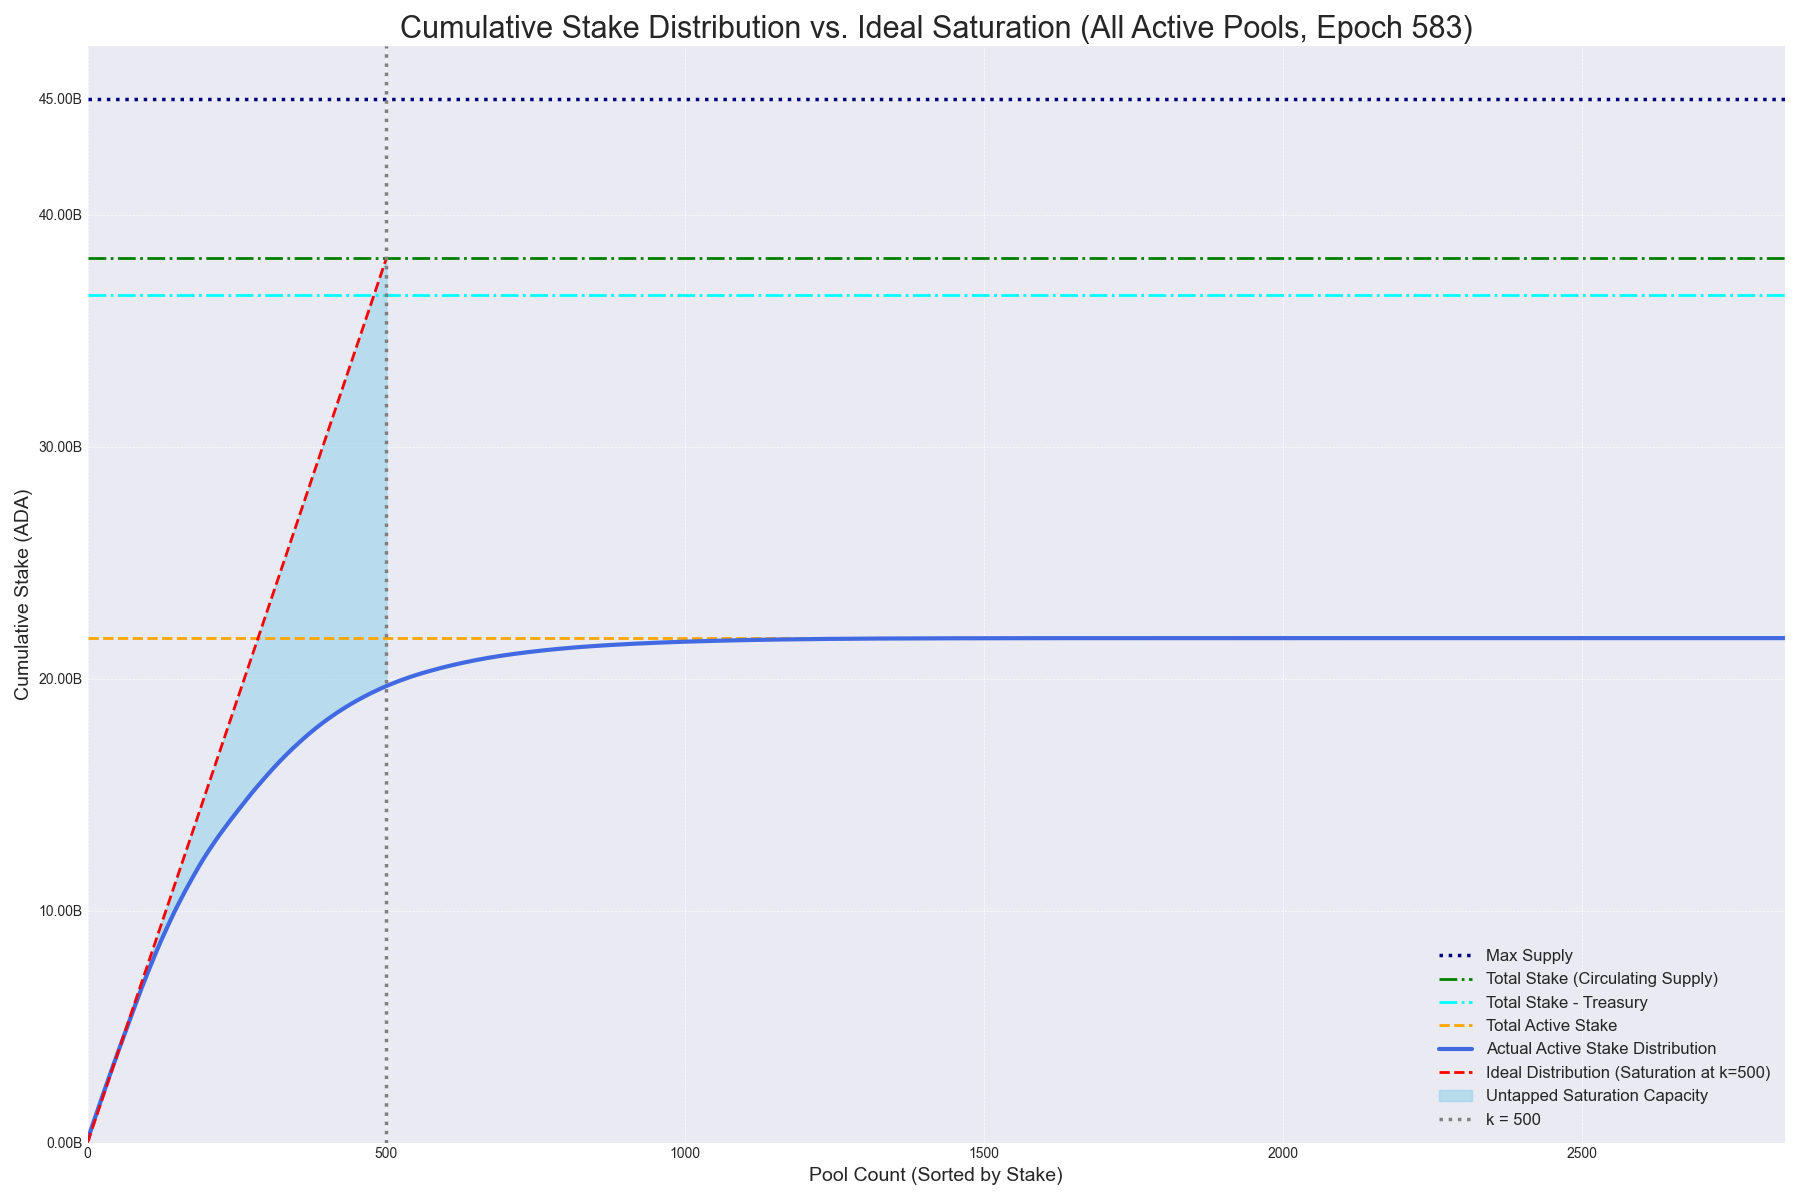
\includegraphics[width=\textwidth]{img/cumulative_stake_distribution_epoch_583_annotated.png}
	\caption{Cumulative Stake Distribution vs. Ideal Saturation (Epoch 583). The chart highlights the
		significant gap between the total circulating supply (less treasury) and the total active stake. This ~16B ADA
		in non-participating capital is the primary constraint for more saturated pools and makes it harder for smaller pools to grow.}
	\label{fig:cumulative-stake}
\end{figure}

The chart above clearly visualizes the primary constraint on the incentive
system. The gap between the ``Total Stake - Treasury'' line (approximately 38B
ADA) and the ``Total Active Stake'' line (approximately 22B ADA) represents
\textbf{16 billion ADA} that is not delegated.

With a circulating supply of approximately 38B ADA, the saturation point for a
pool at $k=500$ is approximately 76M ADA\@. Saturating 500 such pools would
require all 38B ADA to be actively delegated. With only approximately 22B ADA
actively staked, the maximum number of pools that could theoretically be
saturated is:

\begin{equation}
	\text{Max Saturated Pools} = \frac{\text{Total Active Stake}}{\text{Saturation Point}} = \frac{22,000,000,000}{76,000,000} \approx 289
\end{equation}

The more direct consequence is a capital-constrained environment for the active
delegation market. With a finite 22B active ADA, a small or new pool
can only grow by persuading delegators to re-delegate from established, healthy pools.

This is a challenging proposition due to significant incumbent
advantages and delegator inertia. Larger pools offer a proven history of
consistent block production and reliable rewards, making them the rational
choice for financially-motivated, risk-averse or passive delegators. This
dynamic creates a constant tension within the ecosystem: a community of smaller stake
pool operators, many driven by ideological alignment and a desire to contribute, finds
itself in direct competition for a limited resource against the network's most
successful incumbents. Thus, the 16B ADA's absence from consensus does not merely limit
the theoretical number of saturated pools; it fundamentally defines the competitive landscape,
creating a high barrier to growth for new entrants and sustaining the
``viability gap'' observed in the on-chain data.

Cardano is not unique in having a significant portion of its circulating supply outside of consensus.
In fact, it appears to be a consistent characteristic across major
Proof-of-Stake (PoS) blockchains. A comparative analysis of staking data from a
major exchange reveals that Cardano's participation rate is among the highest
in the industry.

\begin{figure}[H]
	\centering
	\captionsetup{justification=centering}
	\begin{tabular}{ccc}
		% --- Row 1: Cardano, Solana, Ethereum ---
		\begin{minipage}{0.3\textwidth}
			\centering
			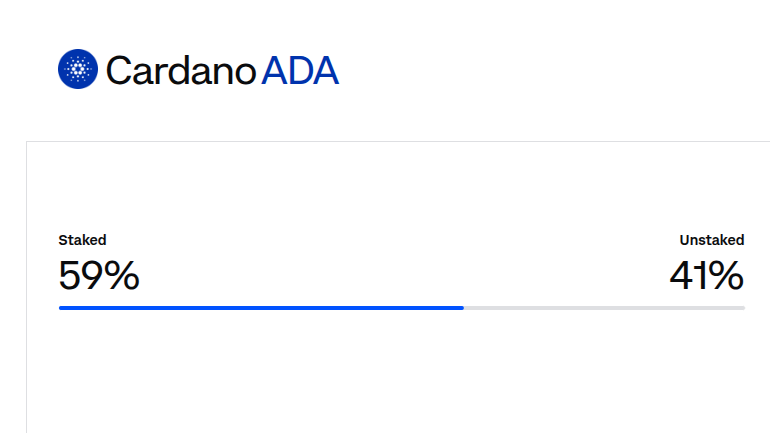
\includegraphics[width=0.9\linewidth]{img/cardano.png}
			\caption*{Cardano}
			\href{https://www.coinbase.com/earn/staking/cardano}{\texttt{\scriptsize Source: Coinbase}}
		\end{minipage}  &
		\begin{minipage}{0.3\textwidth}
			\centering
			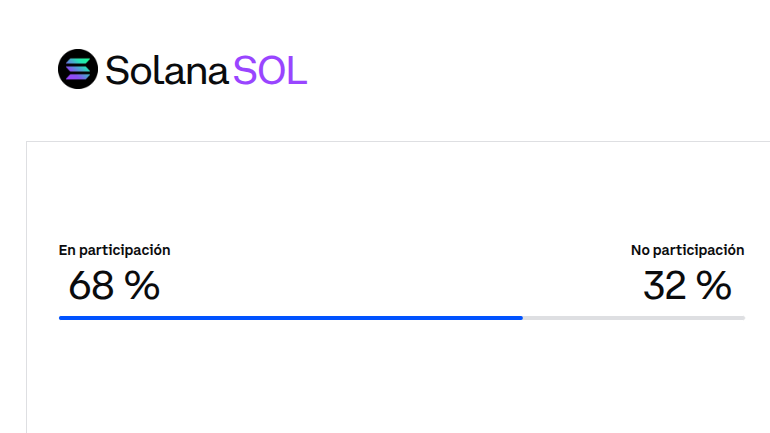
\includegraphics[width=0.9\linewidth]{img/solana.png}
			\caption*{Solana}
			\href{https://www.coinbase.com/earn/staking/solana}{\texttt{\scriptsize Source: Coinbase}}
		\end{minipage}   &
		\begin{minipage}{0.3\textwidth}
			\centering
			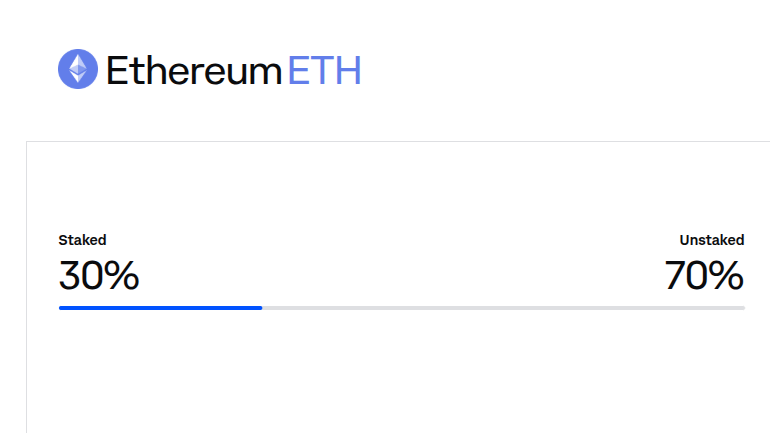
\includegraphics[width=0.9\linewidth]{img/ethereum.png}
			\caption*{Ethereum}
			\href{https://www.coinbase.com/earn/staking/ethereum}{\texttt{\scriptsize Source: Coinbase}}
		\end{minipage} \\

		\addlinespace[2ex] % Add a little vertical space between rows

		% --- Row 2: Polkadot, Cosmos, Avalanche ---
		\begin{minipage}{0.3\textwidth}
			\centering
			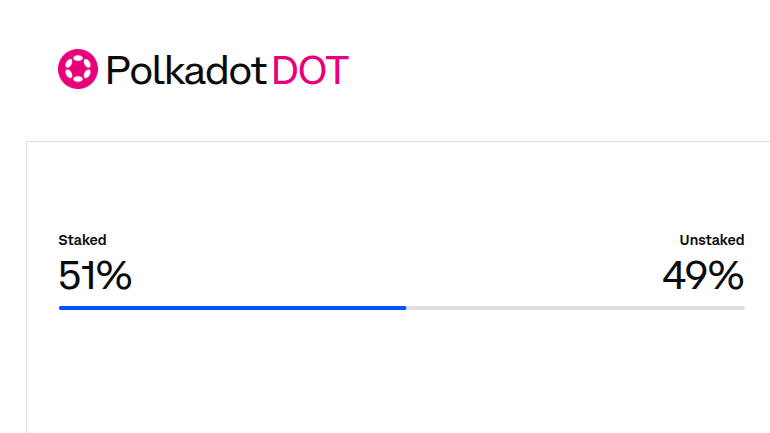
\includegraphics[width=0.9\linewidth]{img/polkadot.png}
			\caption*{Polkadot}
			\href{https://www.coinbase.com/earn/staking/polkadot}{\texttt{\scriptsize Source: Coinbase}}
		\end{minipage} &
		\begin{minipage}{0.3\textwidth}
			\centering
			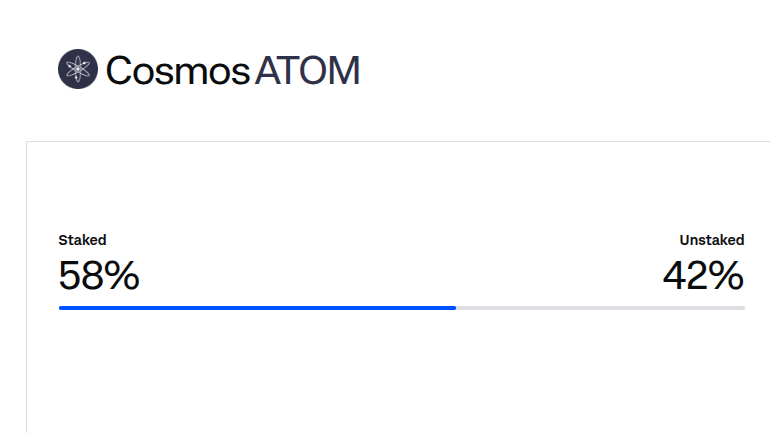
\includegraphics[width=0.9\linewidth]{img/cosmos.png}
			\caption*{Cosmos}
			\href{https://www.coinbase.com/earn/staking/cosmos}{\texttt{\scriptsize Source: Coinbase}}
		\end{minipage}   &
		\begin{minipage}{0.3\textwidth}
			\centering
			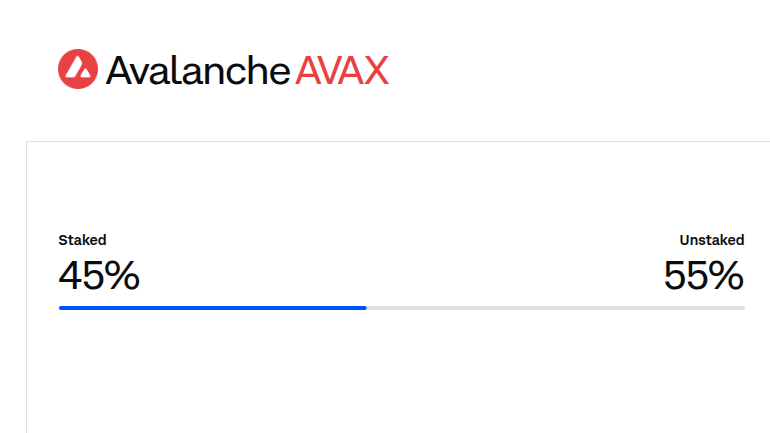
\includegraphics[width=0.9\linewidth]{img/avalanche.png}
			\caption*{Avalanche}
			\href{https://www.coinbase.com/earn/staking/avalanche}{\texttt{\scriptsize Source: Coinbase}}
		\end{minipage}
	\end{tabular}
	\caption{Comparative analysis of staking participation rates across major Proof-of-Stake networks as of October 2025. Cardano's participation rate is notably high relative to its peers.}
	\label{fig:pos_comparison}
\end{figure}

\subsubsection*{A thought experiment: Impact of full stake delegation}

To understand the impact of this capital constraint, it is useful to
conduct a thought experiment and consider what would happen if the 16B
undelegated ADA were suddenly to enter the system.

\begin{enumerate}
	\item \textbf{Initial shock and saturation cascade:} The influx of stake would rapidly flow to the most desirable pools,
	      quickly saturating and then oversaturating the largest operators.
	\item \textbf{The $k$ parameter at play:} As the top pools become oversaturated, their ROA would begin to decline
	      for all members. The saturation parameter ($z_0$), which is currently a soft ceiling for most, would become a hard economic wall.
	\item \textbf{Capital flows downhill:} Rational delegators from these oversaturated pools would be financially incentivized to
	      move their stake to the next-best-performing unsaturated pools. This would create a cascade of delegation flowing down the ranks.
	\item \textbf{The ``Long Tail'' shrinks:} Many pools in the lower tiers would find themselves suddenly viable as they attract
	      new and re-delegated stake, rapidly growing towards mid-level sizes.
\end{enumerate}

Characterizing the 16B in undelegated stake is relevant for future protocol enhancements. This
includes identifying its composition (e.g., exchanges, institutional custodians, or individuals) and
the barriers to its participation.

This large pool of dormant capital shapes the competitive landscape for stake
pool operators. While the prevailing strategy involves competing for existing
delegators in a near zero-sum environment, a more productive paradigm would
focus on activating this latent stake. Activating even a fraction of this
capital would represent a positive-sum gain for the entire ecosystem,
simultaneously increasing network security and the viability of smaller pools.

\subsubsection{Registrations and retirements over time}

A historical view of pool registrations versus retirements highlights the
competitive pressures and maturation of the ecosystem.

\begin{figure}[H]
	\centering
	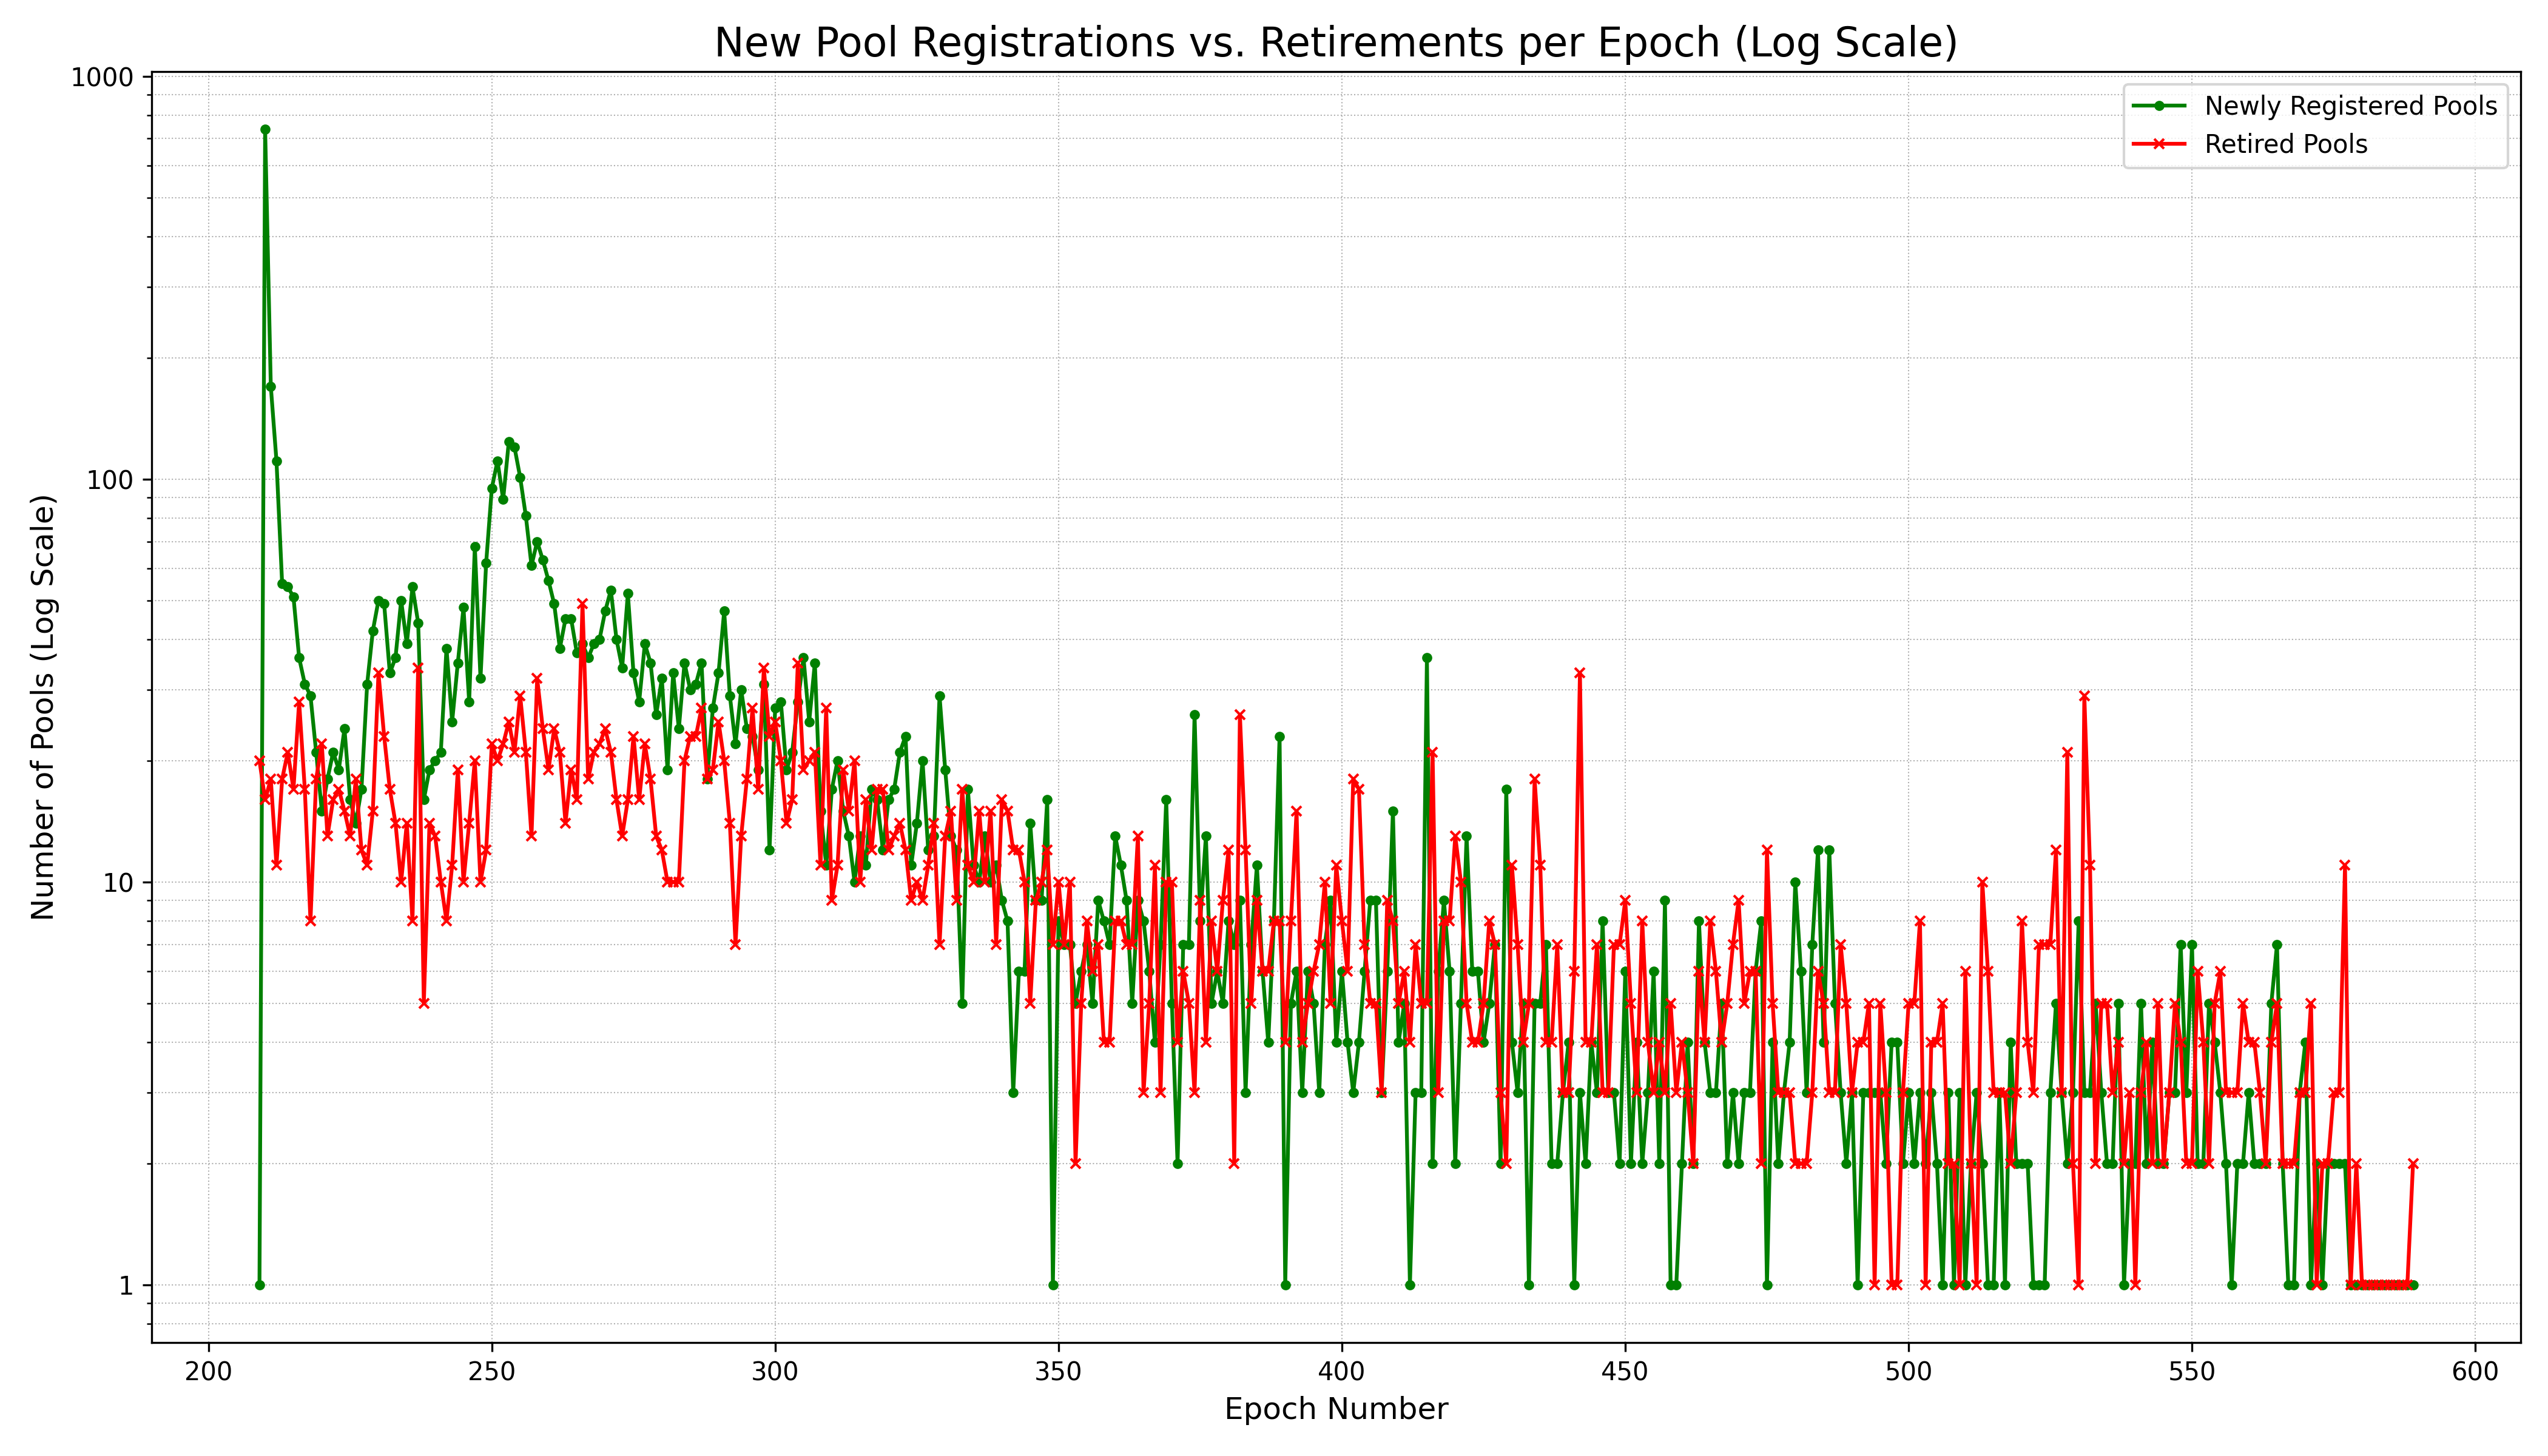
\includegraphics[width=\textwidth]{img/pool_registrations_vs_retirements_log.png}
	\caption{This chart shows the number of new pool registrations (green) versus retirements (red) over time,
		indicating the ecosystem has reached a mature equilibrium.}
	\label{fig:pool-trends}
\end{figure}

The chart shows three phases:
\begin{itemize}
	\item An initial ``boom'' phase (epochs \textasciitilde210-280): New pool registrations
	      outpaced retirements.
	\item A consolidation phase (epochs \textasciitilde280-400): The gap between entries
	      and exits narrowed as the market matured.
	\item A mature equilibrium phase (epochs \textasciitilde400-present): The number of
	      retiring pools consistently matches or exceeds new registrations.
\end{itemize}

This trend suggests the ecosystem has moved from rapid growth to consolidation, reinforcing that the primary
challenge for SPOs today is achieving long-term sustainability in a competitive environment.

\subsection{Analysis of pool parameters}

\subsubsection{Pool cost}

On October 27th, 2023 (epoch 445), the protocol's minimum fixed cost for stake
pools was lowered from 340 ADA to 170 ADA to increase the competitiveness of
smaller pools. An analysis of active pools shows a varied operator response.

\begin{figure}[H]
	\centering
	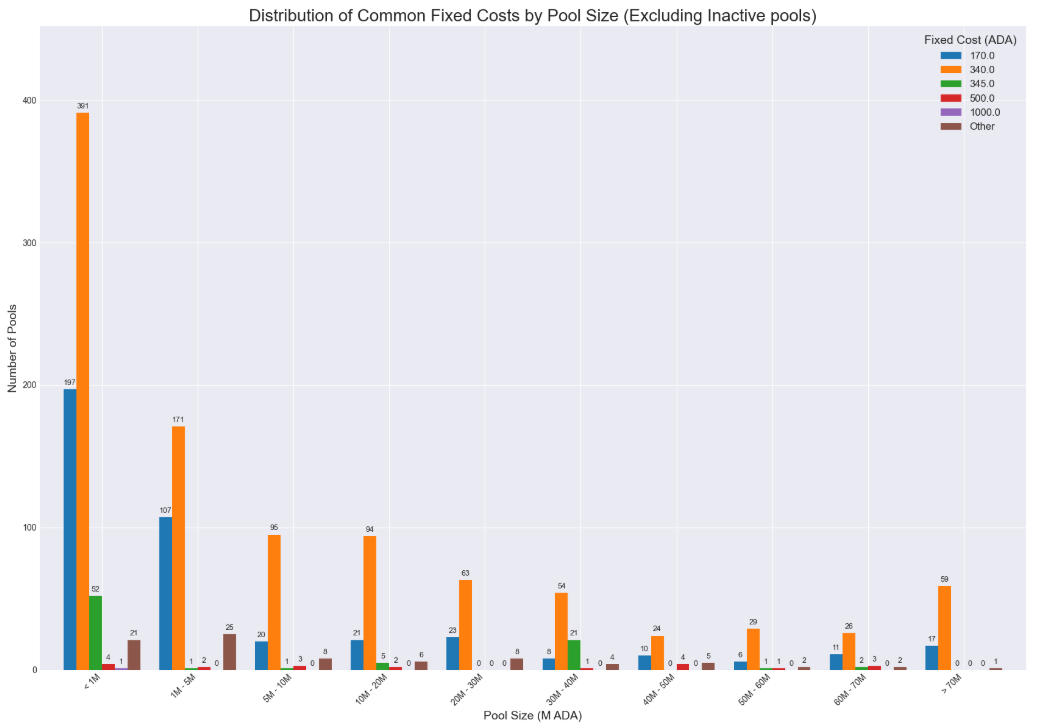
\includegraphics[width=\textwidth]{img/pool-cost-distr.png}
	\caption{Current distribution of common fixed costs by pool size. The chart shows that 340 ADA
		remains the most common fixed cost setting across all active pool sizes.}
	\label{fig:pool-cost}
\end{figure}

Data shows that 340 ADA remains the dominant fixed cost setting for every pool size despite the
availability of the lower 170 ADA minimum. This suggests that 340 ADA is
treated as the standard fee. The 170 ADA fee is the second most
popular choice. The data indicates that the reduction in the minimum pool
cost did not cause a market-wide fee reduction. Instead, it bifurcated the
market into two main tiers:

\begin{enumerate}
	\item \textbf{The incumbents (340 ADA):} Established pools that compete on factors like performance and
	      reputation.
	\item \textbf{The challengers (170 ADA):} Smaller pools using the new minimum as a strategic tool to
	      attract delegation.
\end{enumerate}

IO Research team believe that Min Pool Cost favors Sybil attacks and should be lowered to 0 or removed. 
Which could be paired with the introduction of Min Margin as a new protocol parameter to prevent a 
race to the bottom on fees. 

\subsubsection{Pool margin}

The pool margin, the percentage of rewards taken by the operator, is a key strategic
choice for pool operators. The plot reveals two fundamentally different groups of
pools: a large, competitive market of public pools and relatively small set of private pools.

\begin{figure}[H]
	\centering
	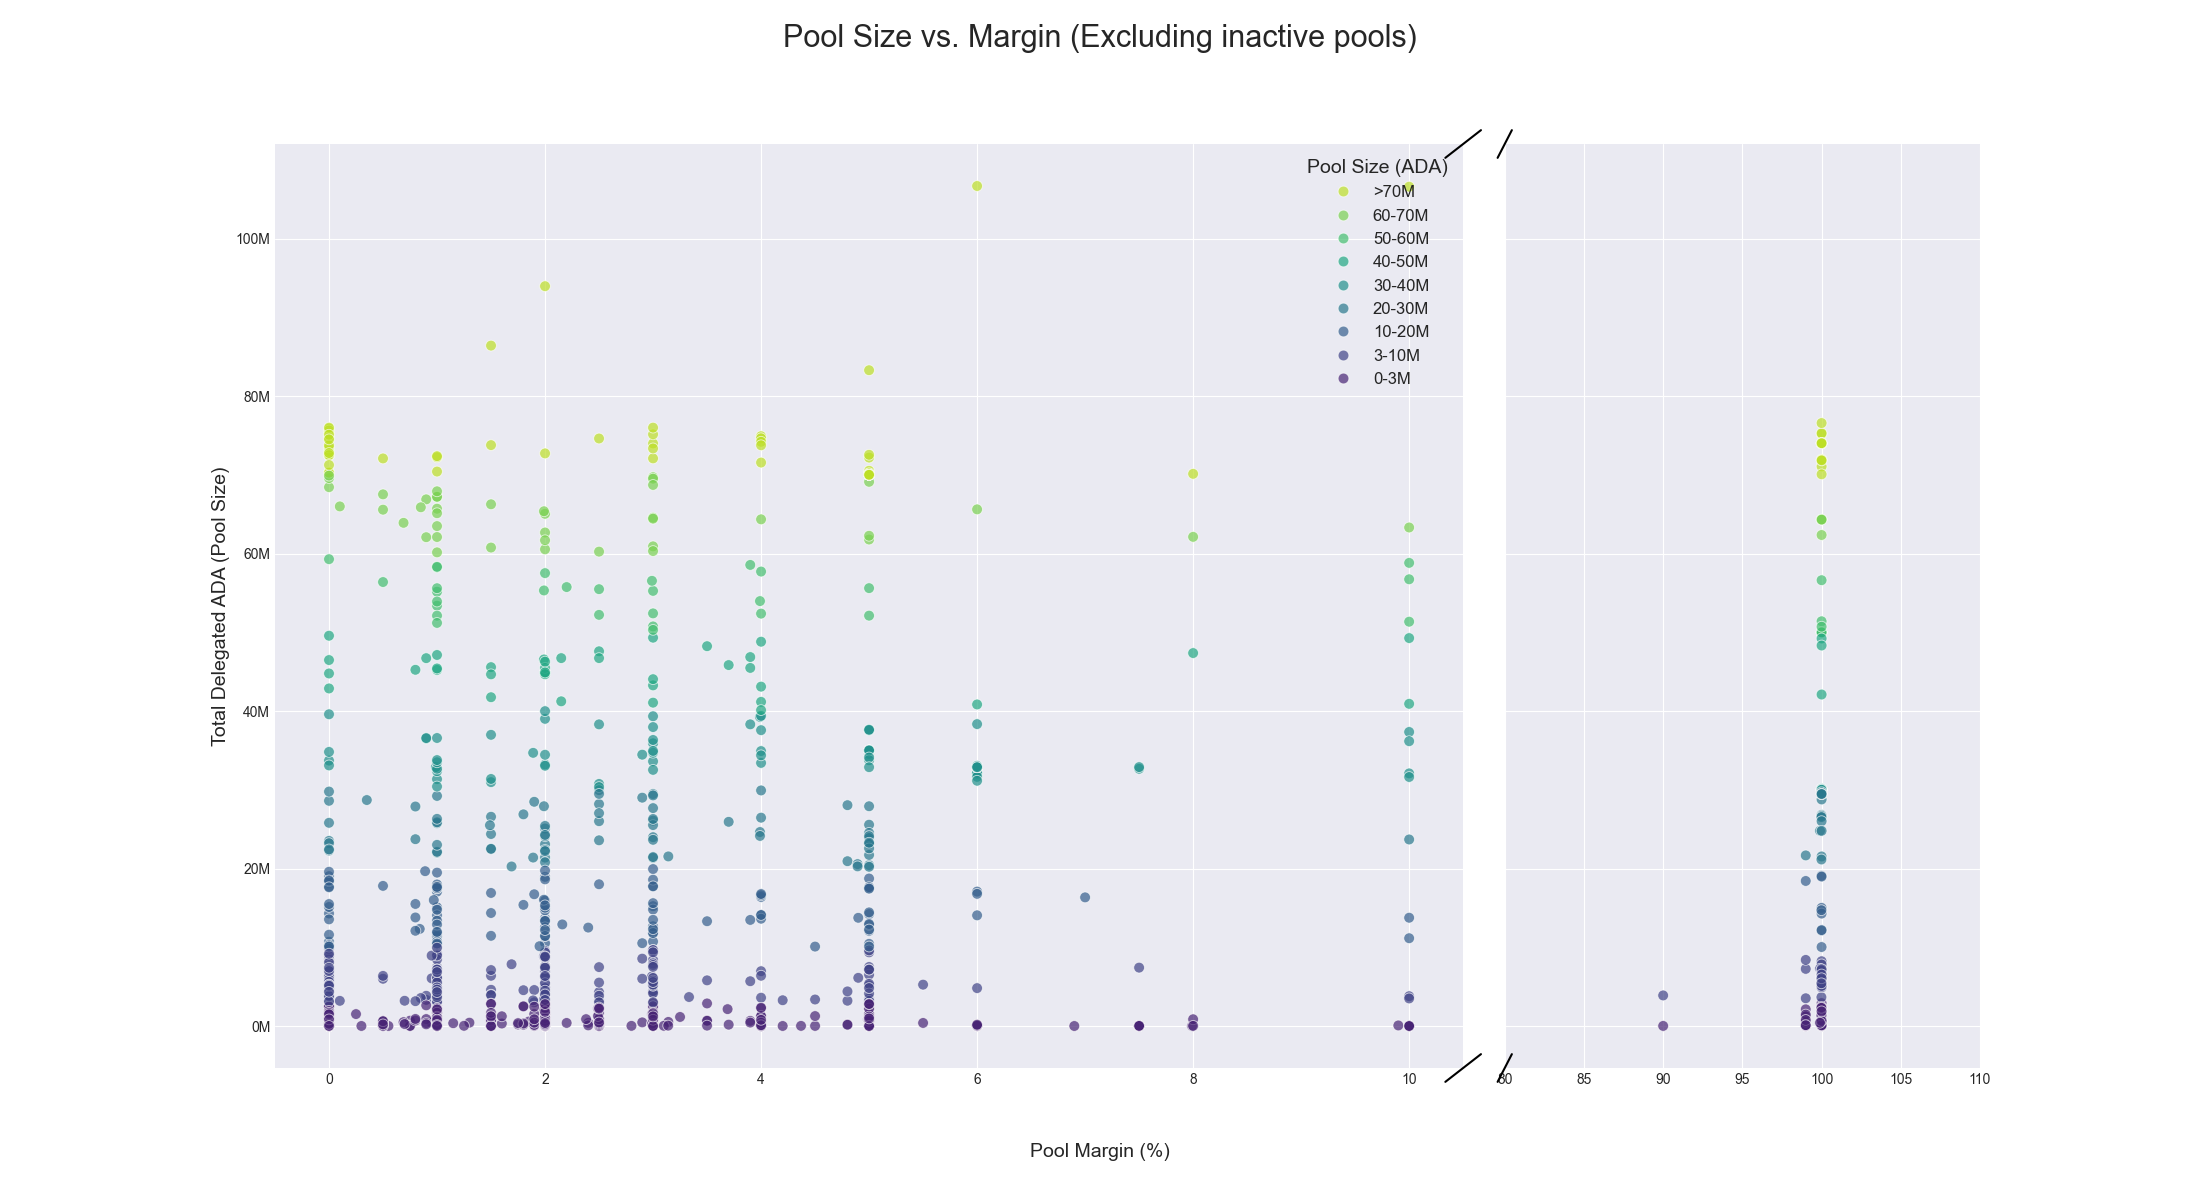
\includegraphics[width=\textwidth]{img/pool_margin_vs_size.png}
\end{figure}

\paragraph{The public market (0-10\% Margin)}
Within the competitive public market, the most significant finding is that
\textbf{pool size does not dictate margin strategy}. Operators of all sizes
can be found at every major strategic fee point.

\paragraph{The 0\% margin strategy}
A dense cluster of pools is visible at the 0\% margin line. Crucially,
these pools span \textbf{every size category}, from the smallest pools to some of the largest,
fully saturated pools on the network. This demonstrates that 0\% margin is not merely a
growth tactic for new pools but a deliberate, competitive choice used by operators
of all sizes to maximize their attractiveness to delegates.

\paragraph{The ``Sweet Spot'' (1-5\%)}
The 1-5\% margin range is the most densely populated part of the
public market. It also features pools from \textbf{every size category}. This
range appears to be the market's stable ``sweet spot,'' representing a standard,
sustainable fee. Operators here, whether large or small, are competing on
factors beyond just the margin, such as reputation, performance, and
community engagement.

\paragraph{The uncompetitive high-margin zone (5-10\%)}
The area \textit{between} 5\% and 10\% is almost entirely empty. This
strongly suggests that margins in this range are uncompetitive and
fail to attract significant delegation, regardless of pool size. The
very small, scattered cluster of pools \textit{exactly at} 10\%
(which also contains pools of various sizes) reinforces this. These are
likely niche outliers, do not seem to be part of a viable public strategy, and are
probably sustained by a small, ideologically-aligned group of delegators or are
friends \& family pools.

\subsubsection{Pool margin vs fixed cost}
The relationship between a pool's margin and fixed cost reveals that operators
adopt one of a few distinct fee strategies, creating clusters of behavior.

\begin{figure}[H]
	\centering
	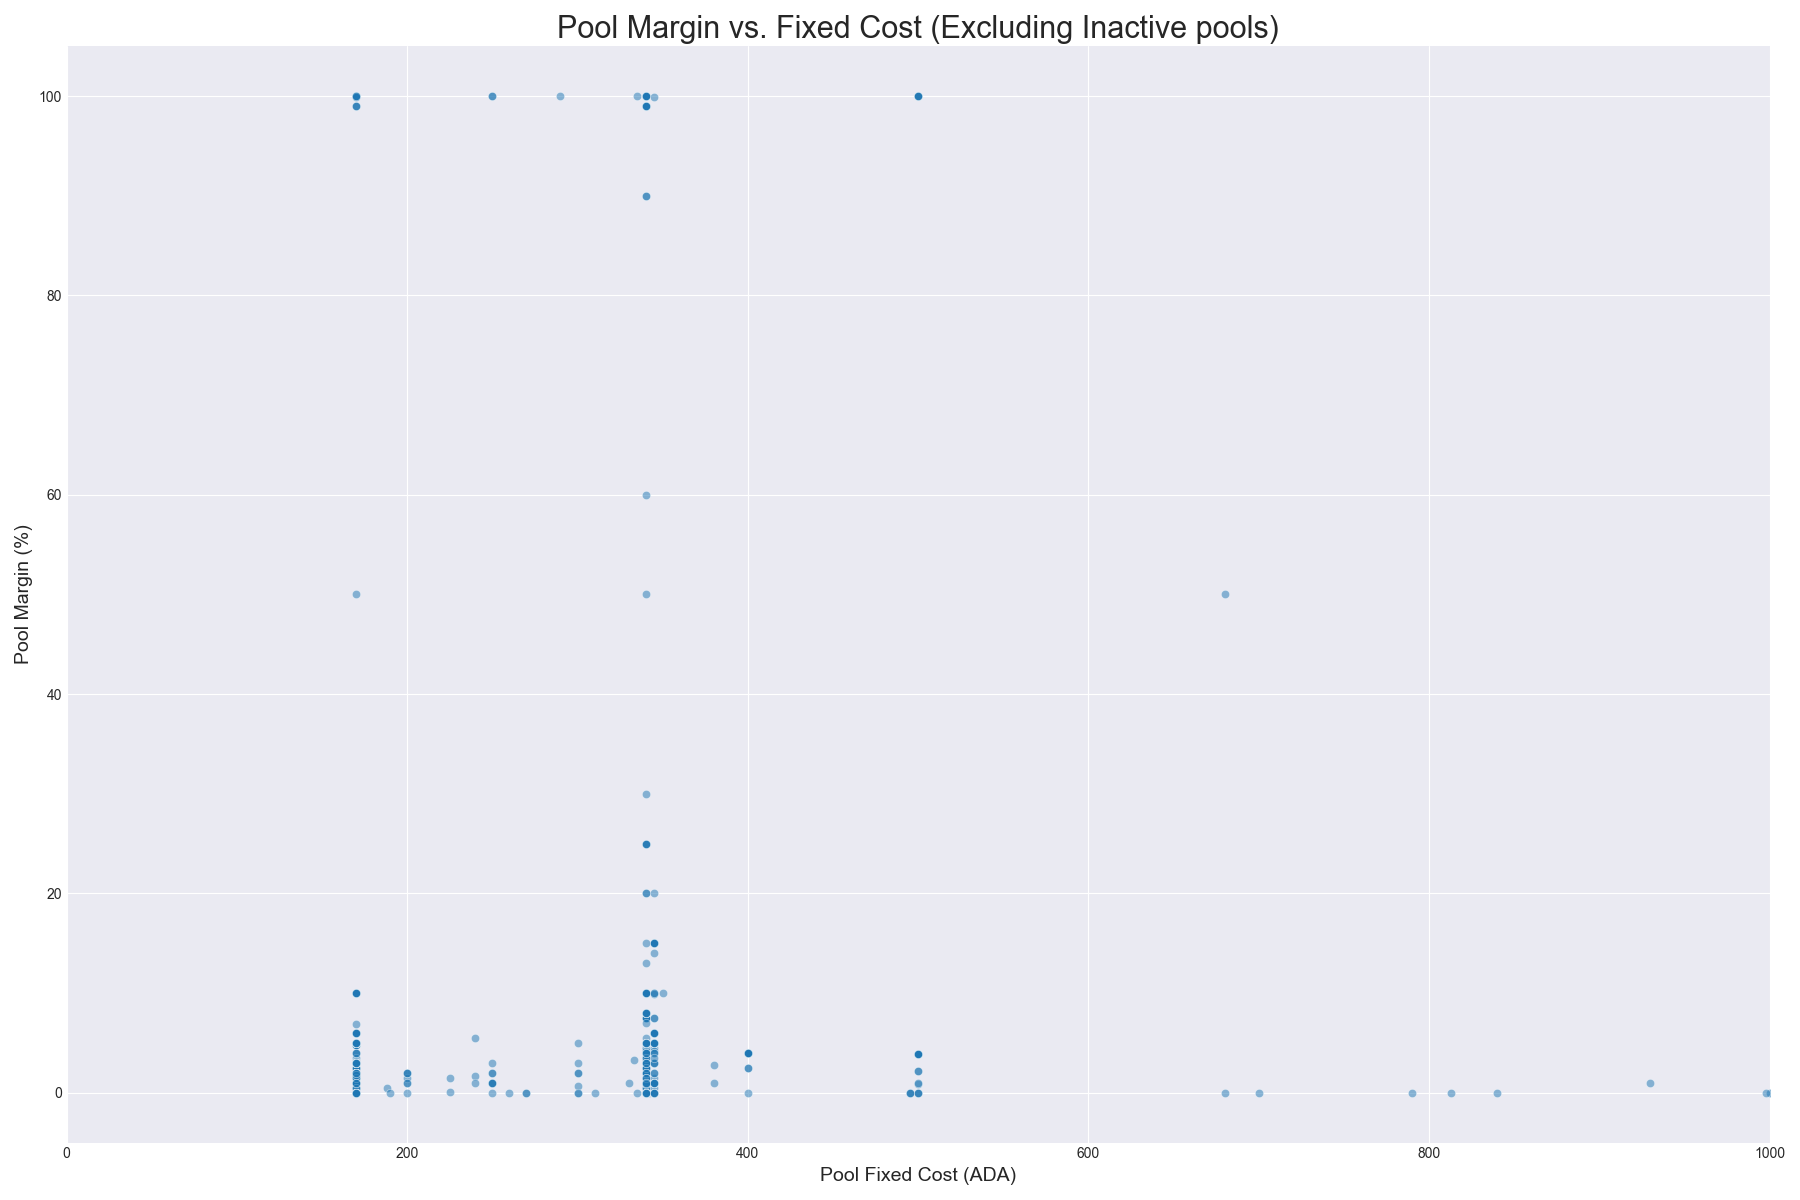
\includegraphics[width=\textwidth]{img/pool_cost_vs_margin.png}
\end{figure}

\begin{itemize}
	\item \textbf{The standard public pool (340 ADA, 0-5\% Margin):} The largest cluster is centered at a
	      340 ADA fixed cost and a low margin, representing the ecosystem's standard.
	\item \textbf{The competitive challenger (170 ADA, 0-3\% Margin):} A second cluster is located at the
	      minimum 170 ADA fixed cost, used by smaller pools to attract initial delegators.
	\item \textbf{The private pool (100\% Margin):} Pool cost is irrelevant for private pools, they will
	      collect all rewards from the pool anyway.
\end{itemize}


Outside of these three strategies, the chart is sparse, indicating that operators see little incentive to
deviate from these established fee packages.

\subsubsection{Pledge}

The incentive design's primary defense against \textbf{Sybil attacks} is the
pledge mechanism, which is intended to make it economically unattractive for an
adversary to create a large number of low-quality pools. By rewarding operators
for committing their own capital ``skin in the game'', the system is designed
to encourage the consolidation of stake into a smaller number of high-quality,
high-commitment pools. To move from this theoretical understanding to a
quantitative one, a simulation was conducted based on the rewards formula
detailed in Section 2.

The simulation calculates the optimal rewards for pools of varying sizes (3M,
10M, 20M, and 76M ADA) across a range of pledge amounts (100k, 1M, 10M, 20M,
and 76M ADA). The results, summarized in Table \ref{tab:pledge-sim}, show the
reward bonus (as a percentage increase over a zero-pledge baseline) that each
pledge level provides for each pool size.

\begin{table}[H]
	\centering
	\resizebox{\textwidth}{!}{%
		\begin{tabular}{@{}lrrrrr@{}}
			\toprule
			\textbf{Pool Size (ADA)}       & \textbf{Pledge 100k ADA}       & \textbf{Pledge 1M ADA}              &
			\textbf{Pledge 10M ADA}        & \textbf{Pledge 20M ADA}        & \textbf{Pledge 76M ADA (Saturated)}             \\ \midrule
			\textbf{3M}                    & 3,923 ADA ($\Delta$ +0.039\%)  & 3,934 ADA ($\Delta$ +0.31\%)        & - & - & - \\
			\textbf{10M}                   & 13,037 ADA ($\Delta$ +0.039\%) & 13,149 ADA ($\Delta$ +0.31\%)       &
			14,354 ADA ($\Delta$ +3.13\%)  & -                              & -                                               \\
			\textbf{20M}                   & 26,036 ADA ($\Delta$ +0.039\%) & 26,147 ADA ($\Delta$ +0.31\%)       &
			27,352 ADA ($\Delta$ +3.13\%)  & 28,634 ADA ($\Delta$ +6.21\%)  & -                                               \\
			\textbf{76M (Saturated)}       & 98,168 ADA ($\Delta$ +0.039\%) & 99,280 ADA ($\Delta$ +0.31\%)       &
			111,332 ADA ($\Delta$ +3.92\%) & 124,158 ADA ($\Delta$ +7.79\%) & 233,634 ADA ($\Delta$ +30.00\%)                 \\ \bottomrule
		\end{tabular}
	}
	\caption{Simulated pledge reward bonus ($\Delta$Rewards \%) by pool size and pledge amount. The table shows
		the calculated optimal rewards and the percentage increase over a zero-pledge baseline.}
	\label{tab:pledge-sim}
\end{table}

The simulation confirms that the economic impact of pledge is non-linear and
varies with a pool's size.

\begin{itemize}
	\item \textbf{Marginal impact of small pledges:} For smaller pools and for pledges under 1M ADA, the reward
	      bonus is marginal (e.g., +0.039\% for a 100k pledge), an amount unlikely to be a deciding factor for
	      delegators.
	\item \textbf{Exponential scaling at saturation:} As pools grow and the pledge amount increases, the bonus
	      scales significantly. For a nearly saturated pool (76M ADA), a 10M ADA pledge yields a +3.92\% reward
	      bonus. Pledging the entire pool's stake results in a +30.00\% bonus.
\end{itemize}

This dynamic confirms that the pledge mechanism discourages sybil attacks by
creating a greater return for consolidating stake into one large,
highly-pledged pool. However, it also introduces a competitive advantage for
well-capitalized operators, contributing to the ``viability gap'' for smaller
operators.

It's worth noting that the pledge bonus does not bring more rewards from the
Reserves to the Rewards Pot, but rather allocates a larger share of the Rewards
pot to the high-pledge pools.

\subsubsection{Pledge in practice}

To empirically validate the simulation's findings, we analyzed on-chain
performance data from all active pools over a 36-epoch period. The methodology
for this analysis, detailed in \href{https://github.com/input-output-hk/spo-incentives/blob/main/spo_incentives/appendixC.txt}{Appendix C}, 
was designed to isolate the economic impact of pledge from other variables. For each epoch, we grouped pools of
similar size into performance-matched cohorts that had produced the
\textbf{exact same number of blocks}, allowing for a direct comparison of how
pledge affects the rewards of otherwise equally performing pools.

The on-chain data provides a confirmation of the simulation's core prediction: the reward
bonus from pledge scales \textbf{non-linearly} with pool saturation and pledge size.
The following case studies illustrate this dynamic, showing that while the impact is functionally
irrelevant for the vast majority of operators, it becomes a dominant economic
factor at the high end of the spectrum.

The analysis of cohorts with lower block production shows that the economic
impact of pledge is negligible. For instance, a case study from Epoch 581 found
11 different pools that each produced exactly two blocks. Despite a wide range
of pledge amounts—from 794k ADA down to just 187 ADA—the highest-pledge pool
earned only \textbf{0.07 ADA} more than the lowest.

\begin{figure}[H]
	\centering
	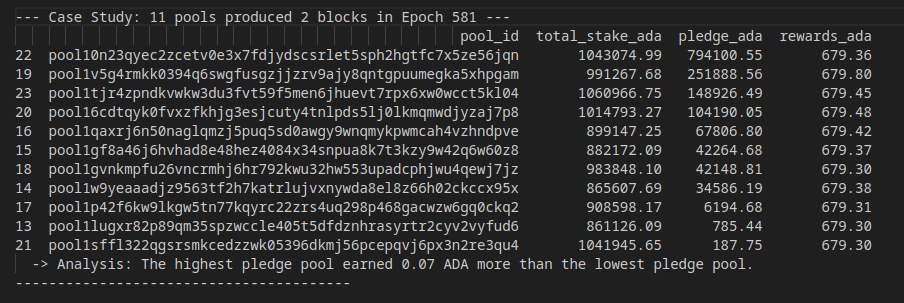
\includegraphics[width=\textwidth]{img/2blocks-e581.png}
	\caption{Case Study: 11 pools producing 2 blocks each in Epoch 581. The reward delta is negligible.}
	\label{fig:2blocks-e581}
\end{figure}

This pattern holds even as performance increases. In a cohort from Epoch 561
where 11 pools produced 13 blocks each, the reward delta attributable to pledge
was still a mere \textbf{1.40 ADA}. These amounts are too small to influence
delegator choice, confirming that for small-to-medium-sized pools, pledge does
not function as a meaningful differentiator.

\begin{figure}[H]
	\centering
	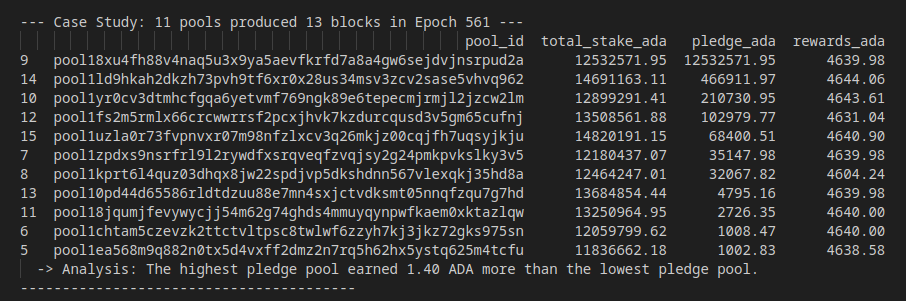
\includegraphics[width=\textwidth]{img/13blocks-e561.png}
	\caption{Case Study: 11 pools producing 13 blocks each in Epoch 561. The reward delta remains insignificant.}
	\label{fig:13blocks-e561}
\end{figure}

Even for pools producing a significant number of blocks, the pledge bonus
remains marginal unless the pool is also approaching saturation. Two separate
cohorts where pools produced 20 blocks each—one from Epoch 574 and another from
Epoch 575—show reward deltas of only \textbf{26.53 ADA} and \textbf{0.90 ADA},
respectively. These amounts are insignificant compared to the total rewards of
nearly 7,000 ADA per pool.

\begin{figure}[H]
	\centering
	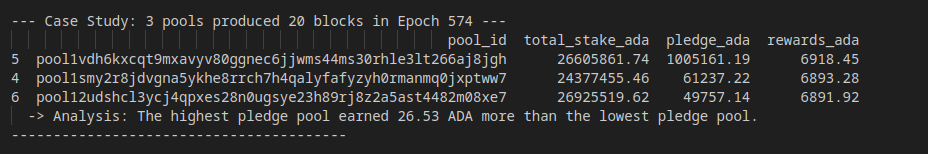
\includegraphics[width=\textwidth]{img/20blocks-e574.png}
	\caption{Case Study 1: 3 pools producing 20 blocks each in Epoch 574.}
	\label{fig:20blocks-e574}
\end{figure}

\begin{figure}[H]
	\centering
	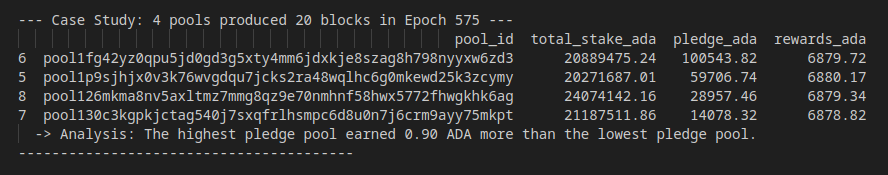
\includegraphics[width=\textwidth]{img/20blocks-e575.png}
	\caption{Case Study 2: 4 pools producing 20 blocks each in Epoch 575.}
	\label{fig:20blocks-e575}
\end{figure}

The effect of pledge only becomes a dominant economic force at the extreme end
of the spectrum, precisely as the simulation predicted. A powerful case study
from Epoch 583 provides the clearest evidence: two nearly saturated pools both
produced exactly \textbf{87 blocks}. The only significant variable was their
pledge. One pool was fully self-pledged with \textbf{\textasciitilde74M ADA},
while the other had a pledge of \textbf{\textasciitilde203k ADA}. The result
was a staggering reward delta of \textbf{8,850.36 ADA} directly attributable to
the larger pledge.

\begin{figure}[H]
	\centering
	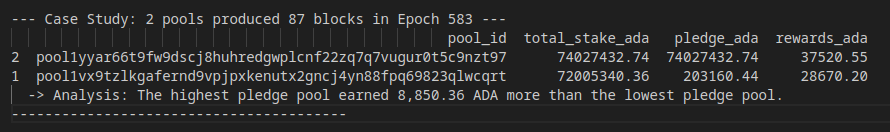
\includegraphics[width=\textwidth]{img/87blocks-e584.png}
	\caption{Case Study: 2 saturated pools producing 87 blocks each in Epoch 583, showing a dramatic reward delta.}
	\label{fig:87blocks-e584}
\end{figure}

These results empirically demonstrate the pledge mechanism is working as designed: it creates
a powerful incentive to consolidate capital into a single, highly-pledged pool while offering a
negligible reward bonus for low-pledge pools, thereby resisting Sybil attacks. However, this
also confirms that for the vast majority of operators who cannot pledge millions of ADA, the
mechanism fails to provide a meaningful ``skin in the game'' signal and creates
a significant competitive advantage for the most well-capitalized actors.

\subsubsection{The influence of apparent performance}
While the analysis shows high-pledge pools earning more, there are isolated
instances where a pool with a higher pledge earns less than a competitor in the
same performance cohort. This highlights the importance of apparent performance
($\bar{p}$)—a measure of blocks produced versus blocks \textit{expected}. A
high-pledge pool that underperforms its statistical expectation can receive a
performance penalty that outweighs its pledge bonus, resulting in a lower final
reward than a low-pledge pool that overperforms. These cases demonstrate that
the incentive structure balances two operator virtues: \textbf{long-term commitment (pledge)}
and \textbf{epoch-to-epoch reliability (performance)}.

\subsection{Analysis of Multi-Pool Operators (MPOs)}

The primary objective of this section is to analyze the influence of large-scale,
professionalized staking entities, commonly known as Multi-Pool Operators (MPOs), on
the decentralization of the Cardano network. This is critical for evaluating the incentive
scheme's effectiveness in mitigating Sybil-like centralization risks.

To focus the analysis on entities with a significant potential for market influence,
this report defines an MPO as any entity operating \textbf{more than five pools}. This scale
indicates a professionalized operation with a strategic approach to market share, distinct from the
organic growth of a single successful pool into a few additional ones. The identification of these MPO
groups was conducted via a heuristic analysis of on-chain data, correlating pools that share
common identifiers in their registration metadata, such as pool tickers, reward addresses, and DNS domain names.

It is important to contextualize the nature of these MPOs. The term is a broad descriptor that
encompasses entities with different motivations. In many cases, these operators have a legitimate
right and even a responsibility to manage a large number of pools. This includes large exchanges providing
custodial staking, which are mandated to maximize returns for their customers (who are, themselves, ADA holders).
It also includes large private funds or individuals staking their own substantial capital. Therefore,
while the concentration of stake under a single MPO is a factor in decentralization metrics, it does not
in itself signify a malicious Sybil attack. The analysis that follows focuses on the observable
on-chain impact of these groups, regardless of their underlying motivation.

\newpage
\subsubsection{MPO stake evolution (Epoch 208-584)}

The two charts tracking Multi-Pool Operator (MPO) stake show the distribution
of stake among all operators running more than five pools.

\paragraph{\% of circulating supply:} The total stake controlled by all MPOs (as defined above)
remains in a stable range, ending the period at approximately 22\% of the total circulating
supply (defined as 45B ADA - Reserves, the basis for calculating the pools saturation point).

\begin{figure}[H]
	\centering
	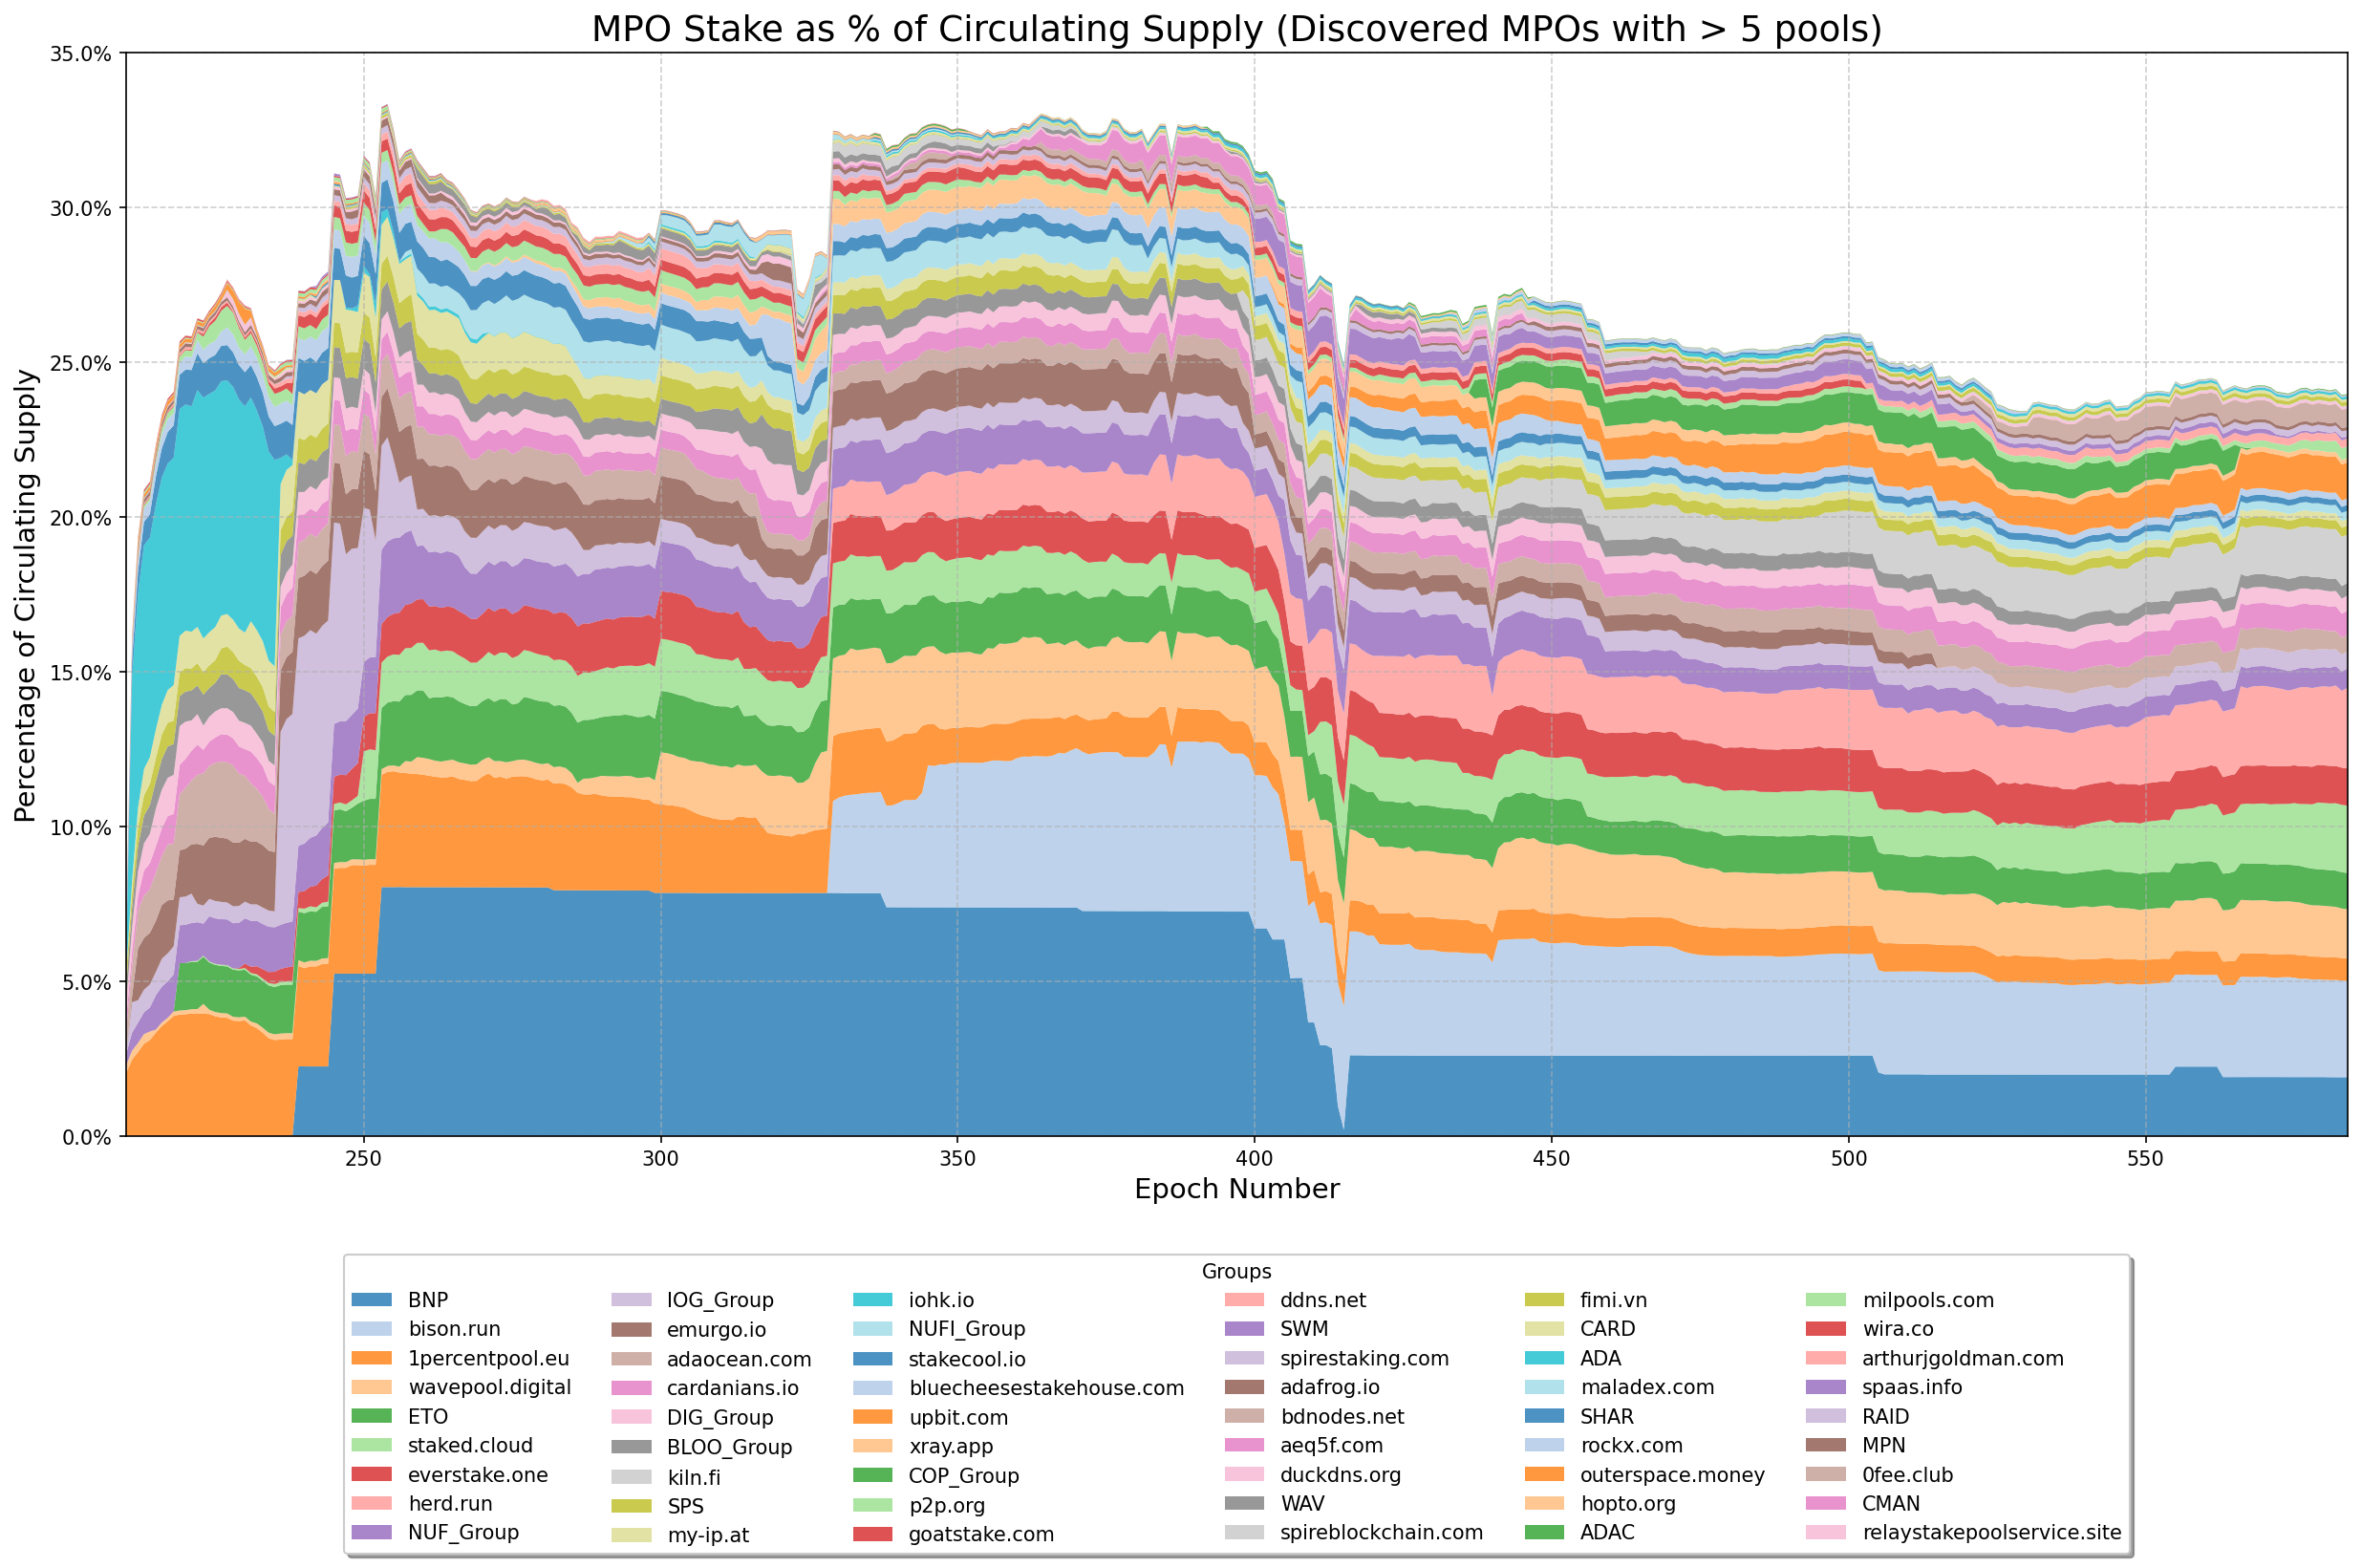
\includegraphics[width=\textwidth, keepaspectratio]{img/mpo_evolution_pct_circulating}
	\caption{MPO Stake as a Percentage of Circulating Supply (Epochs 208-584). This chart shows
		the stability of stake held by large MPOs relative to the total stake (circulating supply).}
	\label{fig:mpo_circulating}
\end{figure}

This level of stake concentration does not pose a risk to network security, as the
Nakamoto Coefficient remains high (see next section). However, it is worth noting that
Section 2.1.5 of the \textit{Shelley-era Delegation and Incentives Design Specification (SL-D1)},
in its discussion of Neutral addresses, states: \textit{\textbf{``We should provide addresses that
		can hold value, but do not contribute to the PoS protocol. Those might be appropriate
		for use by exchanges, which will hold large amounts of value, without legally owning it.''}}
This suggests the specification's authors may not have anticipated that exchanges would eventually
offer custodial staking services (as many now do) or that they would come to hold such large
proprietary amounts of ADA.\@.

\paragraph{Internal Composition:} The internal dynamics of the MPO category show a noticeable
shift around epoch 400. Prior to this, \textit{Binance} and \textit{bison.run} held a significant 13\% of the
stake. However, a substantial drop in their controlled stake at epoch 400 caused a
corresponding decrease in the MPO group's total share. In the period since, the landscape
has stabilized. While these prominent MPOs remain large, the relative market shares among
all major operators have held steady. Notably, no new major multi-pool operators have
emerged, suggesting a mature and potentially consolidated market.

\subsubsection{From the Edinburgh Decentralization Index}

The \href{https://blockchainlab.inf.ed.ac.uk/edi-dashboard/}{Edinburgh Decentralization Index} shows
that Cardano is among the most decentralized blockchains in the industry. Two key metrics
from the index directly relate to our MPO analysis: the Nakamoto Coefficient and the 1-concentration ratio.

\paragraph{Nakamoto Coefficient} The Nakamoto Coefficient, representing the minimum number of
independent entities (pools) required to control 51\% of the stake, shows a consistent and significant
upward trend. It begins the period at a value of approximately 20 and rises to a value
approaching 80 by epoch 584.

\begin{figure}[H]
	\centering
	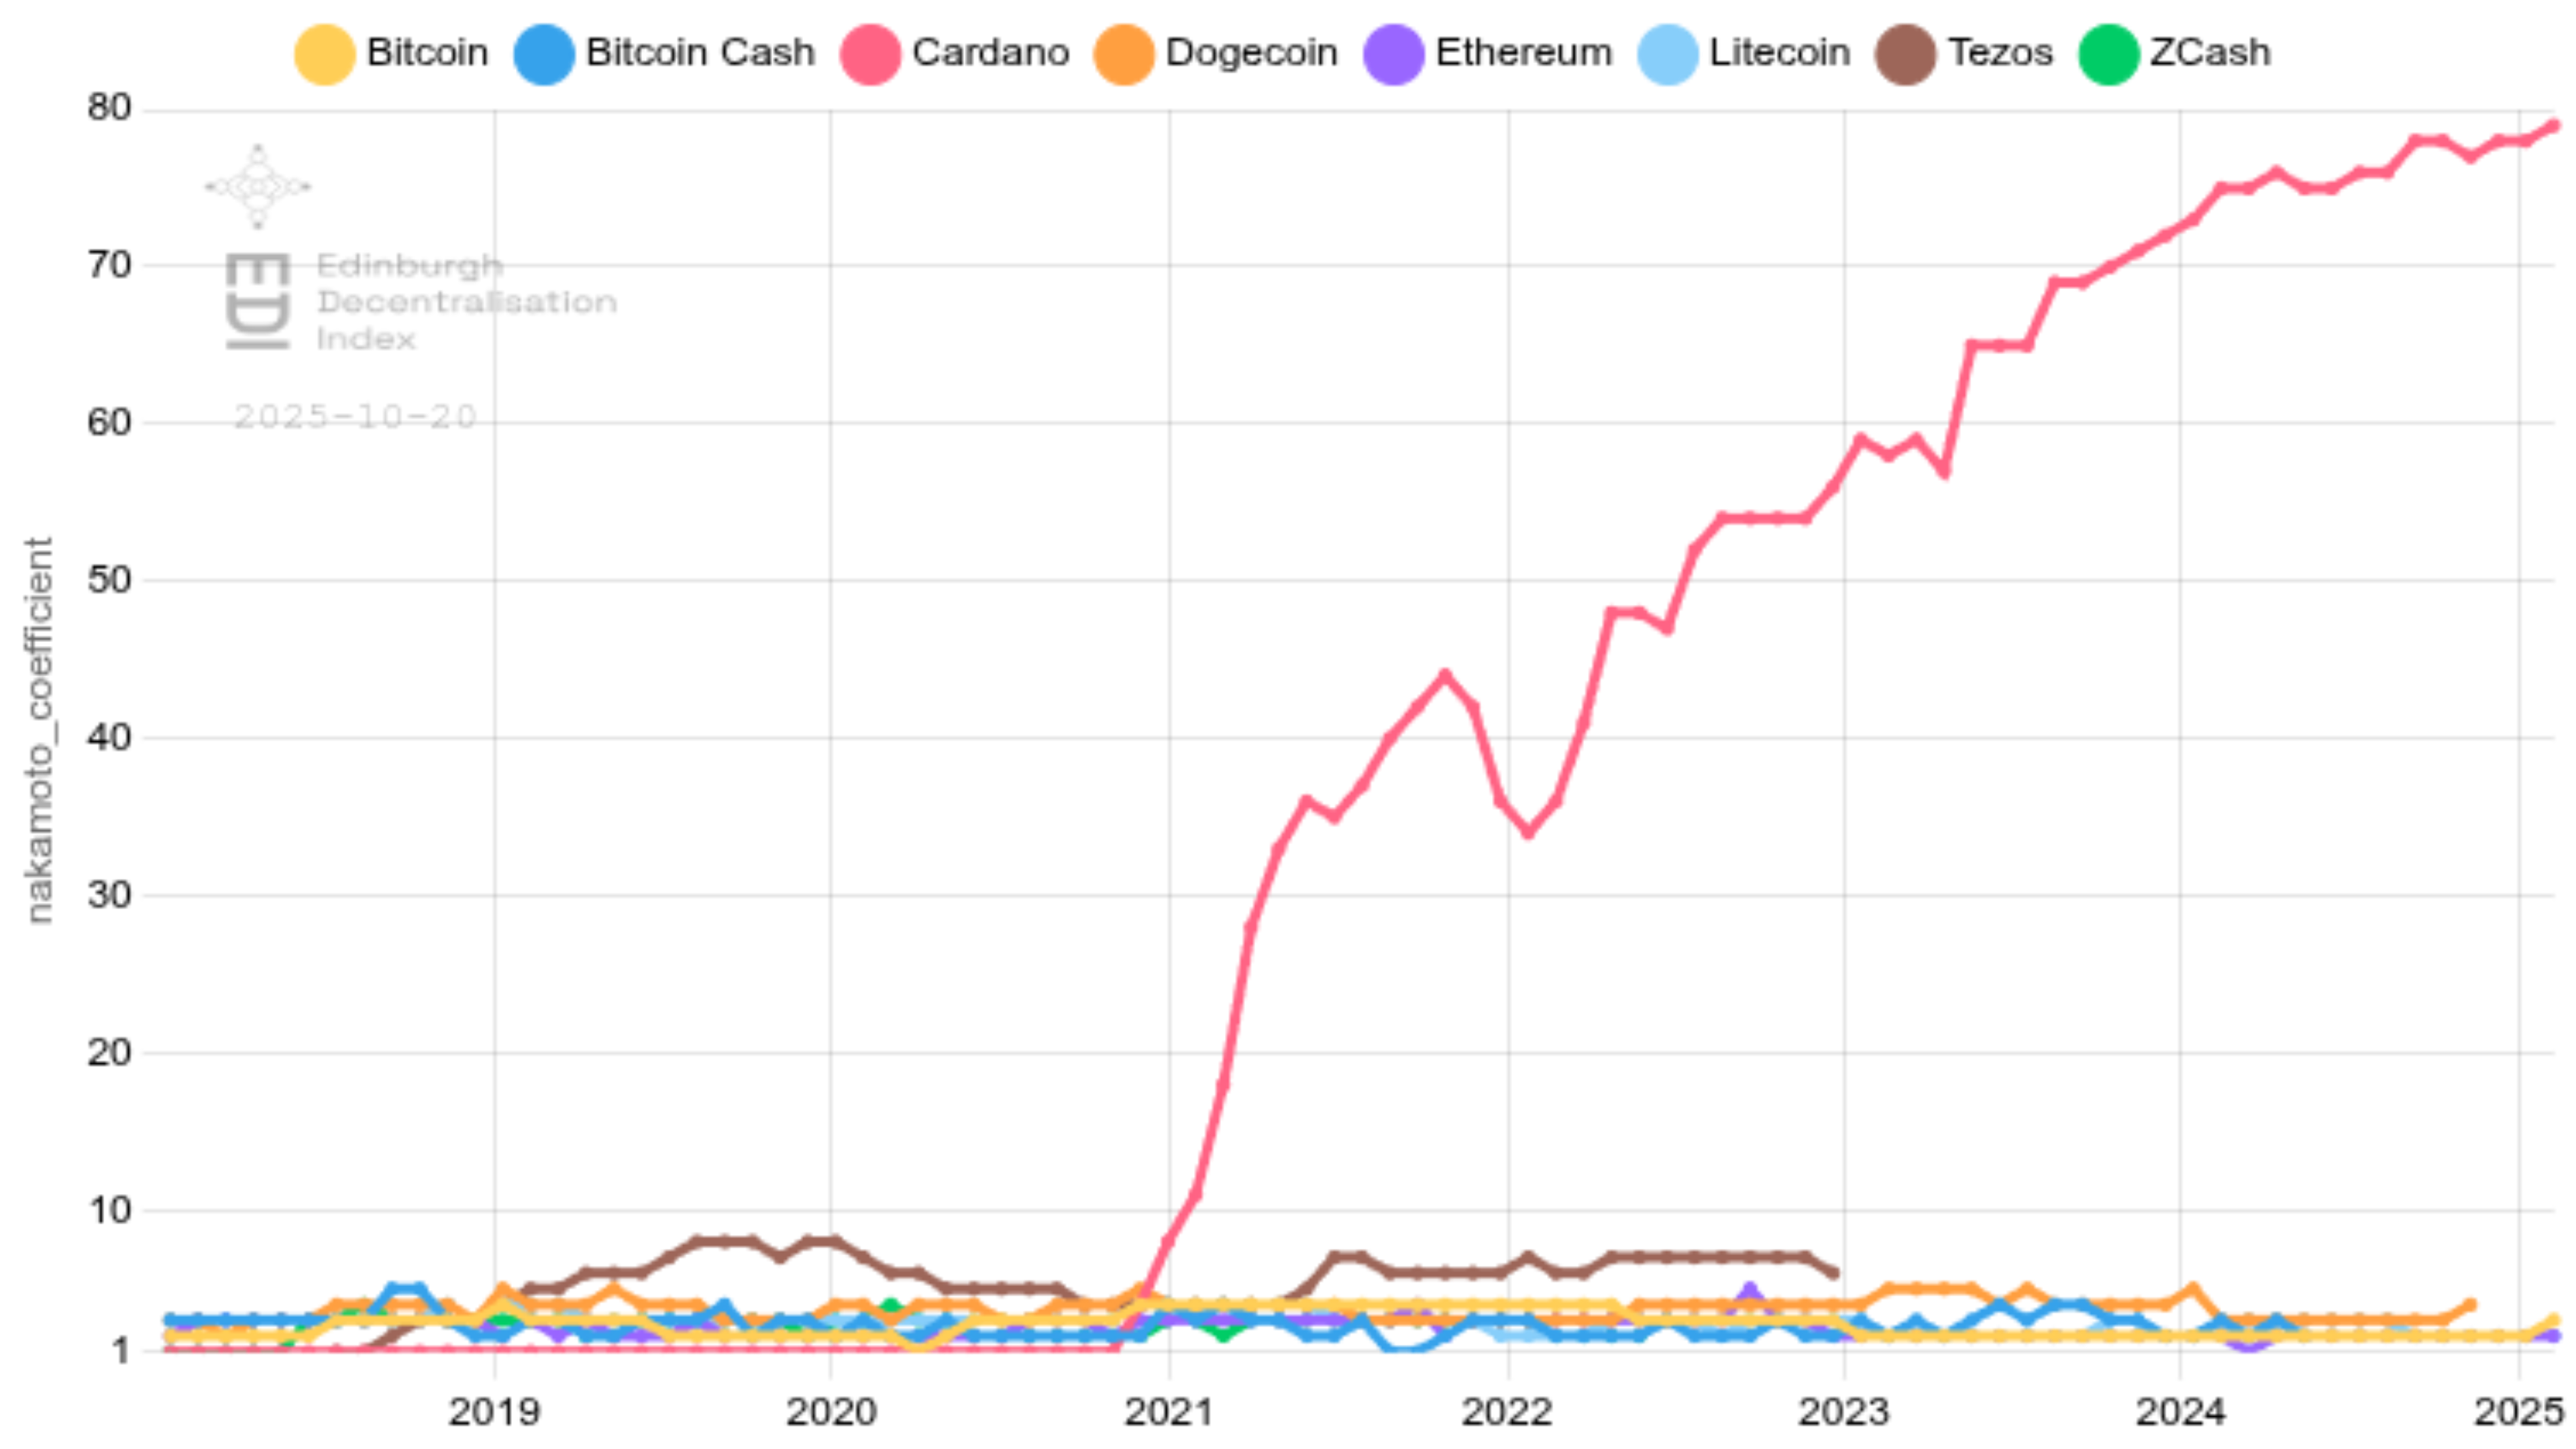
\includegraphics[width=\textwidth]{img/consensus-nakamoto_coefficient-chart.png}
	\caption{Nakamoto Coefficient. The steady increase demonstrates a consistent
		improvement in the network's decentralization and security against collusion.}
	\label{fig:nakamoto}
\end{figure}

\paragraph{1-Concentration Ratio} This chart plots the share of blocks produced by the single
most powerful entity. The on-chain data shows a clear and steady downward trend, starting from
approximately 25\% at the beginning of the period and decreasing to just over 10\% by epoch 584.
This downward slope is a strong indicator of increasing decentralization, as it demonstrates that
the influence of the single largest block producer has consistently diminished over time. This metric,
complementary to the Nakamoto Coefficient, confirms that the network's consensus power
has become progressively more distributed.

\begin{figure}[H]
	\centering
	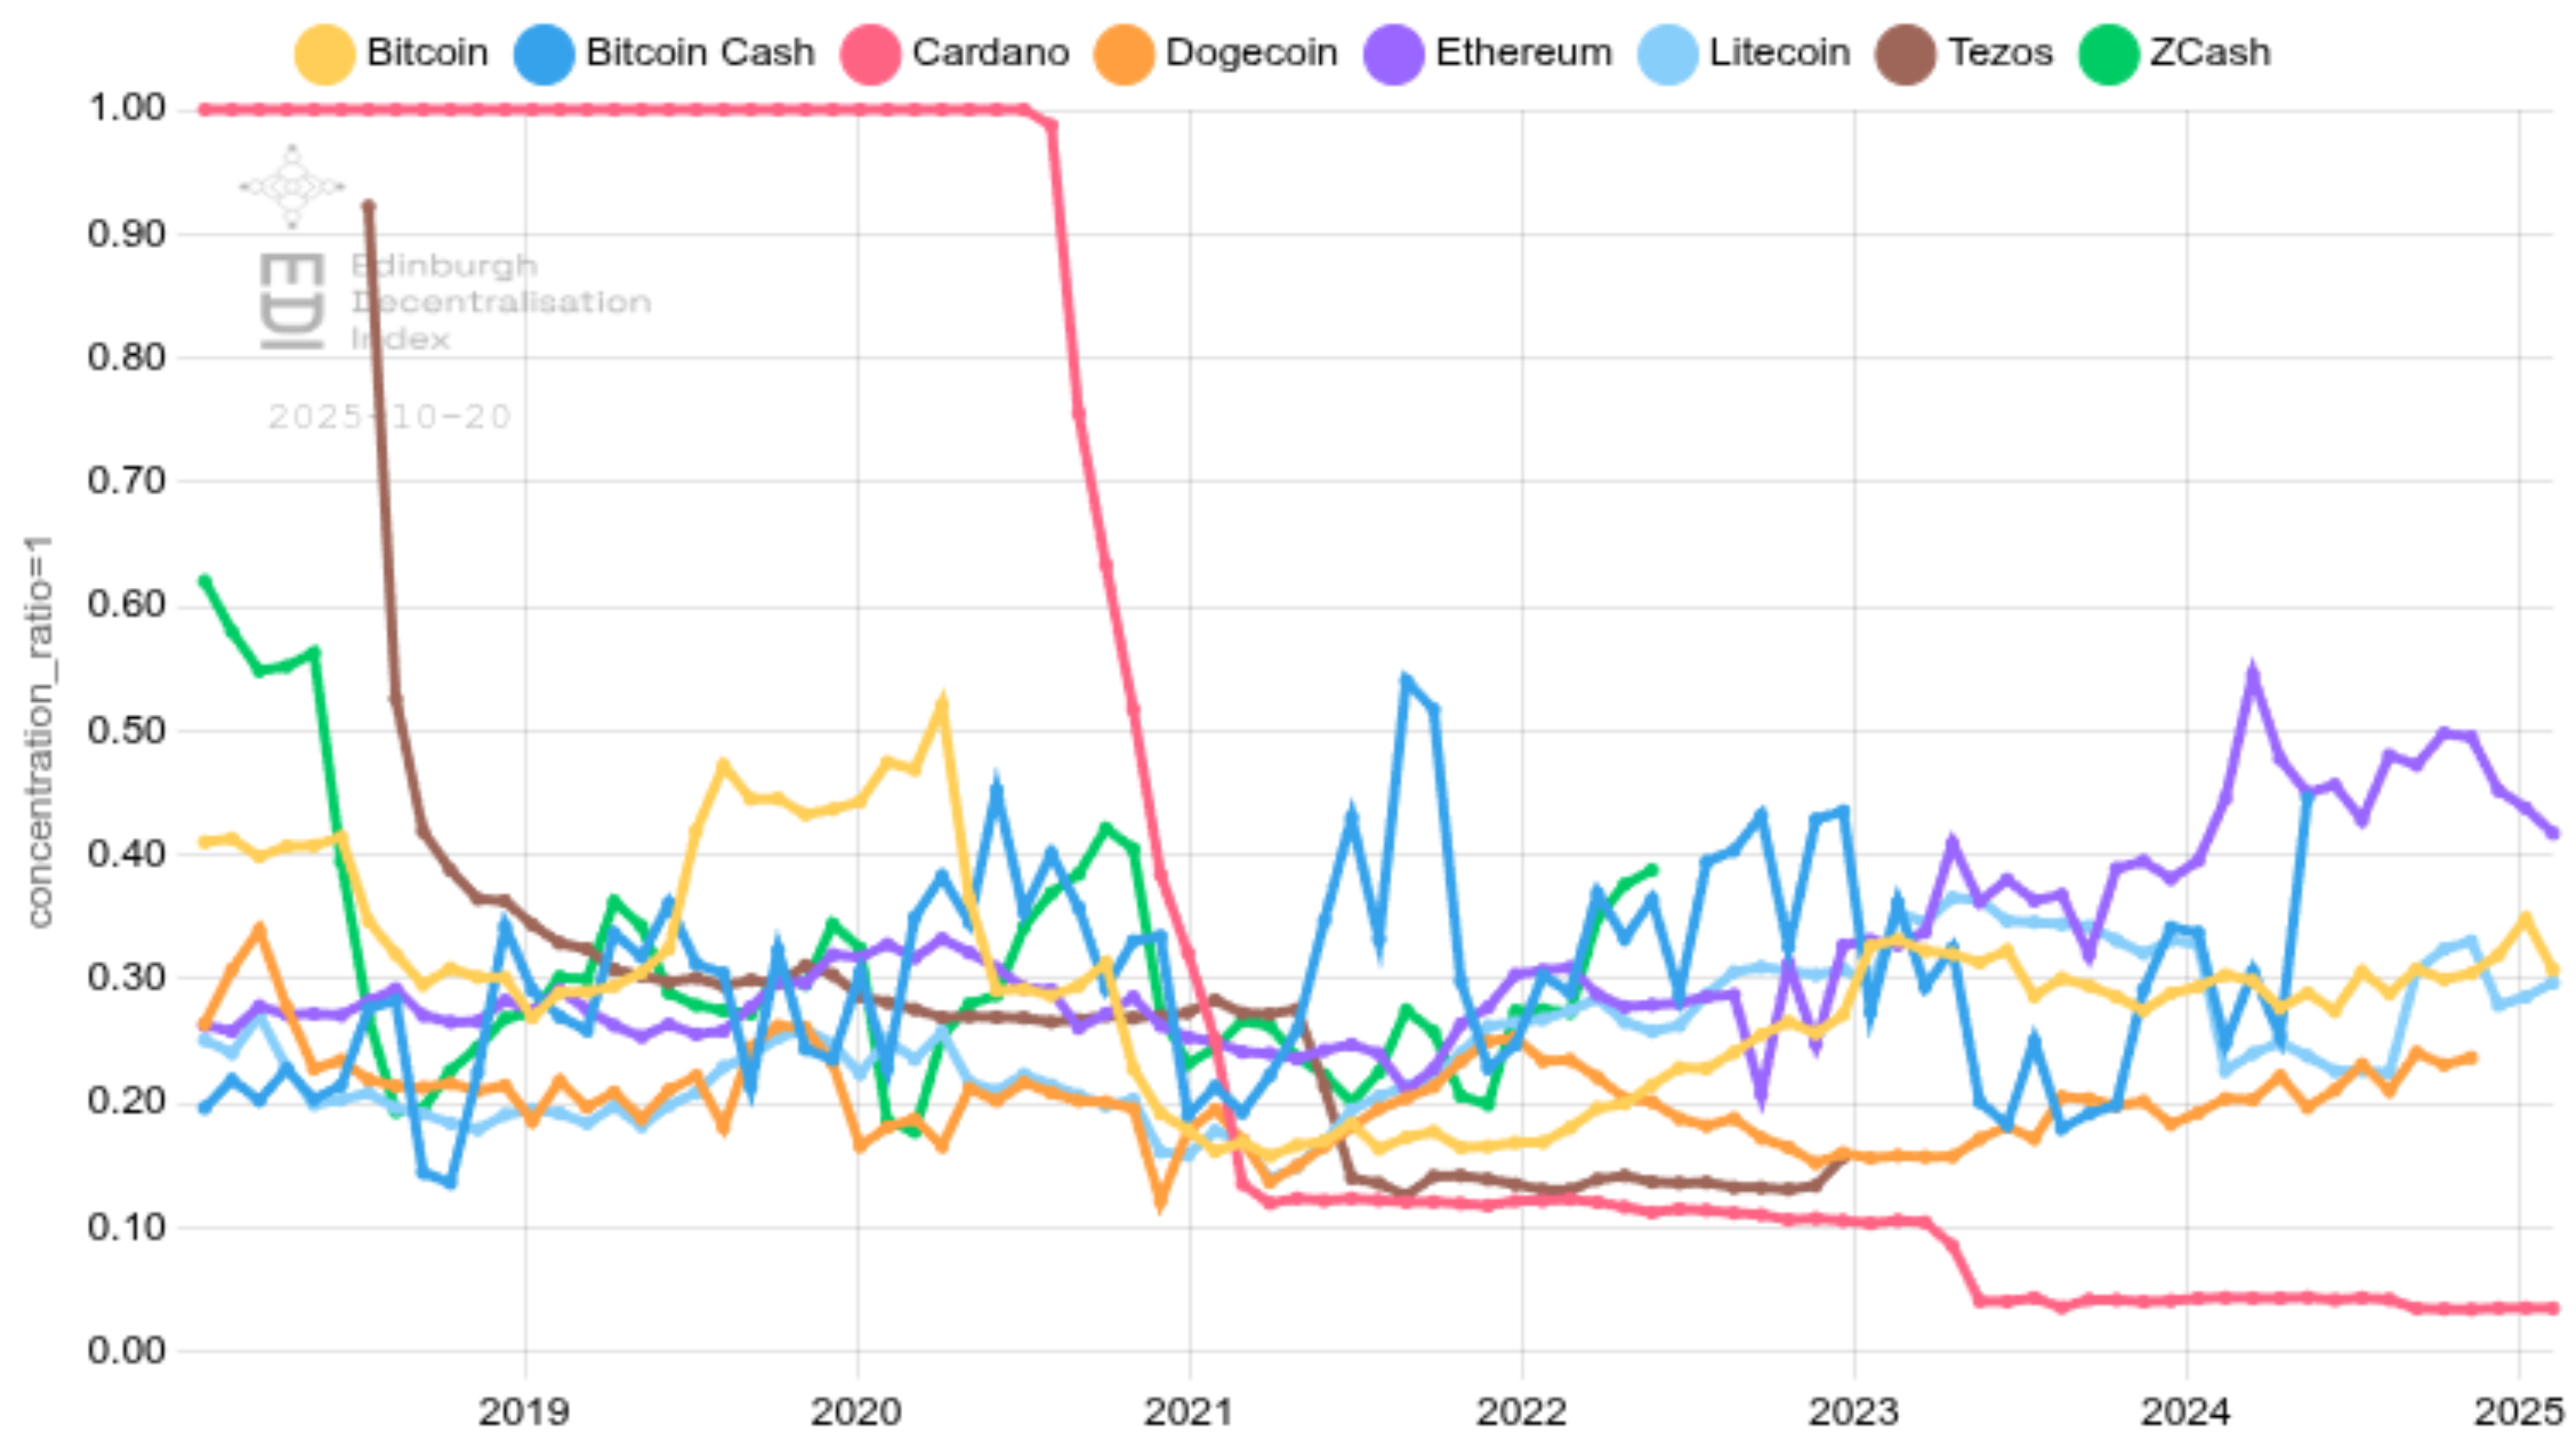
\includegraphics[width=\textwidth]{img/consensus-concentration_ratio=1-chart.png}
	\caption{1-Concentration Ratio. The sustained downward trend indicates a decreasing concentration
		of block production and a corresponding increase in network decentralization over time.}
	\label{fig:k_effective}
\end{figure}

\subsection{Automatic rewards distribution}

The design goal of an automatic and efficient rewards system is one of the most
verifiably successful aspects of the incentive mechanism. Distribution of rewards
is a deterministic protocol function,requiring no manual intervention from either stake pool
operators or delegators. As designed, earned rewards are automatically calculated by the
ledger and credited to the appropriate reward accounts two epochs after the
epoch in which they were generated. This automated process has proven to be
both reliable and efficient, seamlessly distributing rewards each epoch without
causing the transaction bursts or UTXO bloat that the design specification
explicitly sought to avoid. The mechanism's flawless execution in the live
environment serves as direct empirical validation of this core design
principle.

\subsection{Network sustainability trends}

The chart below illustrates key trends related to the sustainability of Cardano's staking reward mechanism, plotting historical data from epoch 208 to 583 and projecting future trends.

\begin{figure}[H]
	\centering
	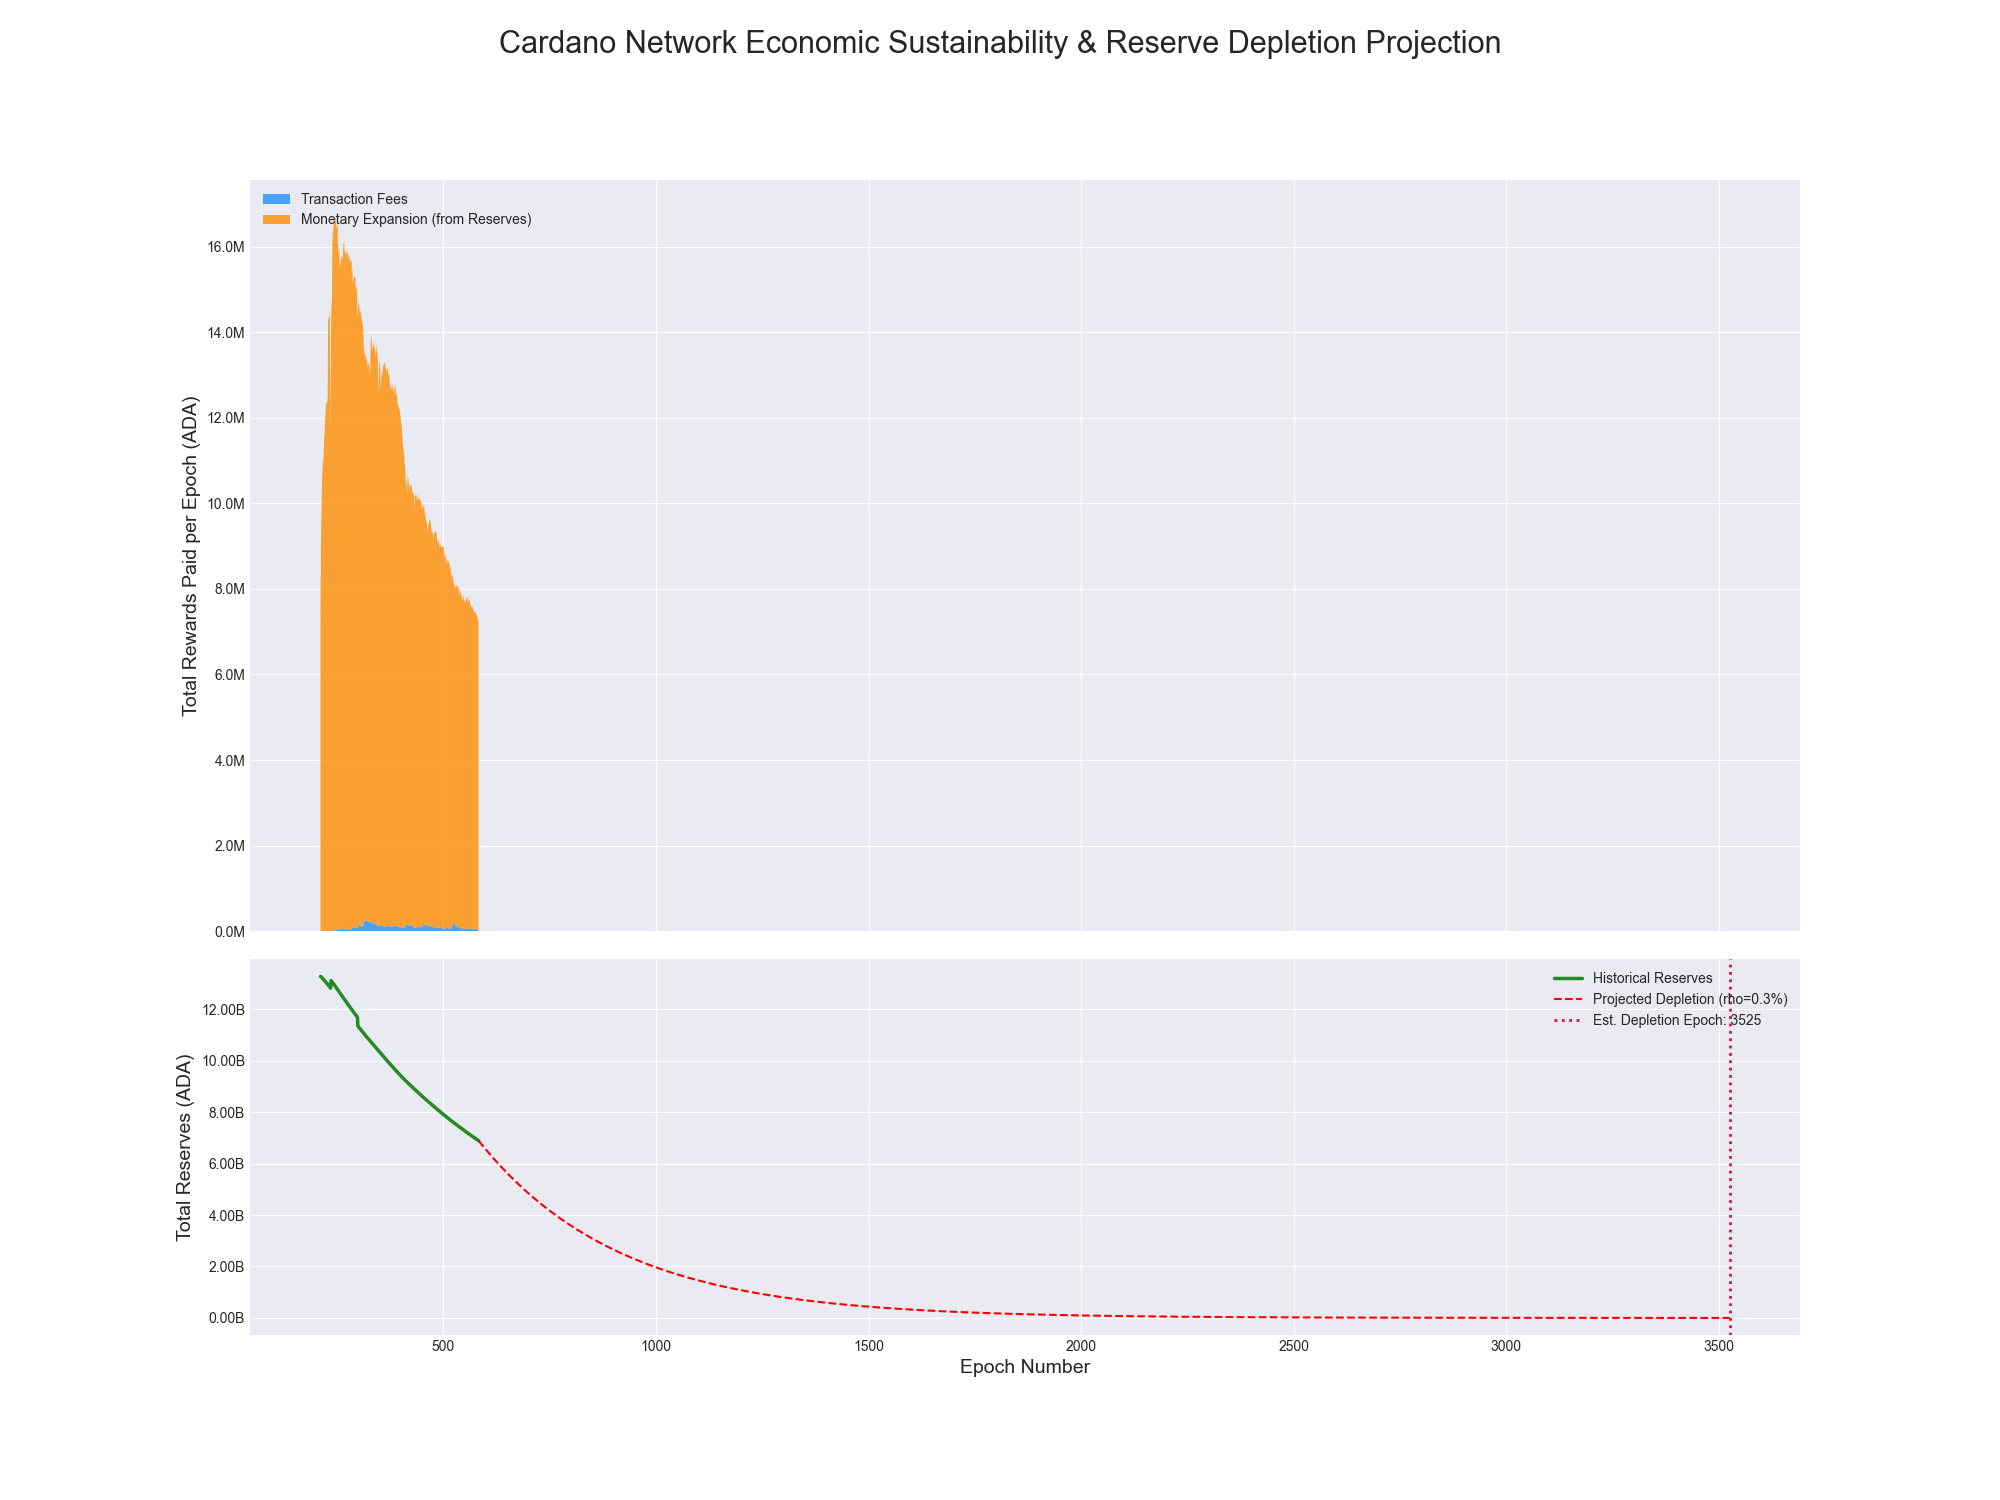
\includegraphics[width=\textwidth]{img/sustainability_trends_with_projection_208-583.png}
	\caption{Cardano reward funding sources and Reserves projection}
	\label{fig:sustainability_trends}
\end{figure}

The top panel clearly shows that the vast majority of staking rewards distributed are currently funded
by monetary expansion drawn from the ADA reserves (parameter $\rho$). Transaction fees contribute only a
minor fraction to the total rewards paid. The bottom panel depicts the historical decline of the ADA reserves
due to this monetary expansion and projects its depletion, estimating reserves will run out around epoch 3500.

These trends highlight a critical need for a new sustainability model. The current heavy reliance
on reserves to fund rewards was designed to bootstrap the network and incentivize
participation during its growth phase. However, as reserves deplete, the network must shift
towards funding rewards primarily through transaction fees. The charts indicate current transaction volume
is insufficient for this. If transaction levels remain at present levels, significant pressure on the reward
system may emerge between epochs 1000 and 1500, well before the projected depletion date. This underscores
the criticality of the upcoming Leios upgrade, which aims to  vastly increase network capacity. While Leios
provides the necessary infrastructure for higher throughput, long-term sustainability hinges on the growth
of the Cardano ecosystem, requiring new applications and use cases to drive the transaction volume
needed to adequately fund staking rewards through fees alone.

\subsection{SPO focus group findings}

Between September 11 and 17, 2025, five focus groups were held with Stake Pool
Operators (SPOs) from around the world, representing a variety of pool sizes
and experiences. These sessions were designed to gather qualitative insights
into the current SPO landscape.

\subsubsection{What motivates stake pool operators}
Across the discussions, a consistent set of motivations emerged:
\begin{itemize}
	\item \textbf{Ideological alignment:} A primary driver is a belief in Cardano's core principles of
	      decentralization and its research-based approach.
	\item \textbf{Technical interest:} Many operators are passionate about technology and view running a pool
	      as a hands-on way to learn and contribute to network infrastructure.
	\item \textbf{Financial incentives:} The potential for revenue is a driver, whether as passive income or a
	      strategic way to acquire ada to cover operational costs.
	\item \textbf{Community engagement:} A desire to engage with the Cardano community, support the ecosystem,
	      and fund real-world projects is a recurring theme.
\end{itemize}

\subsubsection{Key challenges and frustrations}
Despite their motivations, SPOs consistently face a significant set of
challenges:
\begin{itemize}
	\item \textbf{Attracting and retaining delegators:} This was identified as the most common problem.
	      Delegator stake is often ``sticky,'' rarely moving from large or even retired pools, making it difficult
	      for smaller pools to gain visibility and grow.
	\item \textbf{Economic viability and rising costs:} The rising cost of hardware and server maintenance,
	      coupled with declining Return on ADA (ROA), makes it increasingly difficult for SPOs to remain profitable.
	\item \textbf{Centralization and competition:} A concern is the concentration of stake in a few large
	      entities and centralized exchanges, which operate many pools and make it difficult for smaller,
	      community-focused SPOs to compete.
\end{itemize}

\subsubsection{Ineffective protocol parameters}
\begin{itemize}
	\item \textbf{Pledge:} There is widespread frustration that the pledge parameter has little impact on
	      rewards unless the amount is exceptionally large, failing to function as the intended ``skin in the game''
	      mechanism for most operators.
	\item \textbf{Minimum pool fee:} This is a point of contention. While smaller pools rely on the fixed fee
	      to cover costs, it can also deter delegators who see their rewards consumed. 
	\item \textbf{Slow pace of protocol changes:} Operators expressed frustration with the slow progress on
	      implementing improvements to incentive parameters that have been discussed within the community for years.
\end{itemize}

\subsubsection{Discussion of existing proposals}
SPOs provided feedback on several proposals aimed at addressing these
challenges:
\begin{itemize}
	\item \textbf{Minimum margin proposal:} The general sentiment was that a minimum margin could create a
	      fairer environment, but there were concerns that large pools could set their margin to the minimum while
	      smaller pools would need a higher margin to be sustainable.
	\item \textbf{CIP-50 (pledge leverage):} This proposal was generally viewed positively as a way to make
	      pledge more effective, though some worried it could put more pressure on SPOs in a growth phase.
	\item \textbf{Raising the $k$ value:} Increasing the $k$ parameter was contentious. Some saw it as a way to
	      encourage decentralization, while larger pools felt like they would be penalized for their hard work and
	      success.
\end{itemize}

\section{Synthesis and evaluation}
\label{sec:synthesis}

This section synthesizes the findings from the preceding analysis to evaluate the
performance of Cardano's stake pool incentive mechanism. By comparing the theoretical
design goals from section 2 with the empirical on-chain outcomes from section 3, we
can directly address the project's primary objectives and offer an informed conclusion
on the system's health and effectiveness.

\subsection{Evaluating the achievement of design goals}
\label{sec:evaluating-goals}

The incentive mechanism has been a resounding success in achieving its core
\textbf{technical and security goals}, while simultaneously highlighting the
\textbf{divergences between a simplified economic model and the complex, human-driven reality}
of a live ecosystem.

\subsubsection{Observed successes}

\begin{itemize}
	\item \textbf{A highly performant and secure network:} The goal of incentivizing performance
	      and participation has been unequivocally met. The network is reliably secured by 741``Healthy''
	      246``Viable'' stake pools,and 627 pools that are struggling but are ready to produce blocks when called upon.
	      The system consistently achieves an efficiency of over 98\% of block production. The high Nakamoto Coefficient and decreasing concentration ratio further confirm the network is robustly decentralized.
	\item \textbf{Flawless automatic rewards:} The goal of an automatic and efficient rewards system is fully
	      realized. The protocol has functioned flawlessly since inception, distributing rewards every epoch
	      without manual intervention or the negative network effects (like UTXO bloat or transaction bursts) the
	      design specification sought to avoid.
	\item \textbf{Effective Sybil resistance:} The pledge mechanism, as the primary tool for Sybil resistance,
	      works exactly as designed in its primary function. Both simulation and on-chain case studies prove
	      it creates a powerful, non-linear economic incentive to consolidate capital, making the creation
	      of many low-quality pools uneconomical.
\end{itemize}

\subsubsection{Divergences between model and reality}

\begin{itemize}
	\item \textbf{The paradox of pledge:} While an effective Sybil deterrent, the pledge mechanism
	      \textbf{fails as a meaningful ``skin-in-the-game'' signal} for the vast majority of operators. As shown
	      in the analysis, the reward bonus is ``functionally irrelevant'' fo`r pledges under 10M ADA (e.g., deltas
	      as low as 0.07 ADA) , a finding echoed by frustrated SPOs. This creates a severe competitive imbalance,
	      where the mechanism only benefits well-capitalized actors, directly contributing to the ``viability gap''.
	\item \textbf{Equilibrium reality vs. The $k$ expectation:} The expectation of the ecosystem converging
	      on $k$ desirable pools (currently 500) was a theoretical outcome based on a model of perfectly rational
	      economic actors. This is not a design failure, but a clear illustration of the gap between a simplified
	      model and a human-driven ecosystem. The on-chain reality is a more complex, stratified system with 1,614
	      active pools. While not the $k=500$ prediction, the system \textit{has} achieved a
	      \textbf{substantial and stable equilibrium}, characterized by a consistent operator structure and
	      a predictable rate of registrations and retirements. The core issue is that within this stable equilibrium,
	      873 active operators remain below the 3M ADA viability line.
	      \textbf{16B ADA remaining outside the consensus mechanism} is a major real-world factor creating a
	      capital-constrained environment that cements this viability gap.
	\item \textbf{The Complexity of actor behavior:} The assumption of a purely ``rational delegator'' is a
	      necessary simplification used in game theory to allow for formal reasoning about a model. It is not a
	      prediction of individual behavior, as reality is always far more complex. The empirical analysis highlights
	      these complexities.
\end{itemize}

\subsection{Determining the need for protocol changes}
\label{sec:need-for-changes}

The findings indicate that the system requires \textbf{fine-tuning and targeted revisions,
not a complete overhaul}. The fundamental game-theoretic model is sound for its primary purpose:
securing the network.

However, the system is not optimal. The significant divergences—particularly the ineffectiveness
of pledge for most operators and the persistent ``viability gap'', necessitate adjustments. The operator
frustration with the slow pace of change on these known issues underscores this need.

The analysis points toward two avenues for improvement:
\begin{enumerate}
	\item \textbf{Parameter adjustment:} The pledge mechanism fails to provide a meaningful signal
	      for most operators , and fee structures are a point of contention. This suggests a re-evaluation
	      of these parameters is warranted.
	\item \textbf{New on-chain mechanisms:} The ``viability gap'' affecting 873 active but struggling
	      operators points to a structural problem that parameter-tuning alone may not solve. This suggests
	      a need to explore new protocol-level mechanisms, such as the ``virtual pool'' or pool alliance concept,
	      to allow smaller operators to combine resources and compete effectively.
\end{enumerate}

\section{Conclusions and recommendations}

We conclude that the \textbf{most significant \textit{immediate} risk to the network is social,
	not technical}, while a significant \textit{long-term} risk is economic.

\begin{itemize}
	\item \textbf{Technical risk is low:} The network is robustly decentralized and secure. The existence
	      of 741 ``Healthy'' pools far exceeds original design requirements. The analysis of MPOs shows their stake
	      is stable and does not pose a systemic threat to consensus.
	\item \textbf{Social risk is high:} The primary immediate risk is \textbf{operator disillusionment}.
	      This is a direct consequence of the divergences identified above. The large number of active but unprofitable
	      operators (873 pools below the 3M ADA viability line) has created a disenfranchised segment of the community.
	      These operators feel the system is inequitable, citing the pledge paradox (which only benefits whales), the
	      high barrier to consistent rewards, and the struggle against delegator inertia. This social friction is
	      fundamentally rooted in the network's underlying wealth distribution: a small number of wallets control a
	      majority of the delegated stake, and a substantial portion (16B ADA) remains unstaked.
	\item \textbf{Long-Term economic risk:} Beyond the social risk, the analysis confirms a critical
	      long-term \textbf{economic risk: network sustainability}. As detailed in Section 3.8, the current reward
	      model is overwhelmingly subsidized by the ADA reserves, which are on a finite depletion schedule. The
	      network's long-term survival is contingent on a successful transition to a fee-market model, where transaction
	      fees alone are sufficient to incentivize stake pool operators.
\end{itemize}

This places immense importance on the forthcoming \textbf{Leios upgrade}. While Leios is designed to provide the
necessary network capacity for high throughput, it only creates the ``highway'' and does not guarantee the ``traffic''.
The primary long-term risk is a failure to generate the ecosystem growth required to produce sustainable
transaction volume.

This reality suggests a strategic imperative for the community. Ecosystem funds, particularly
the \textbf{Treasury and Project Catalyst}, should consider prioritizing and directing resources
toward identifying and nurturing ``killer apps'' with the potential for mass adoption that
can drive significant on-chain activity in the Leios era. To accelerate this growth, projects should
also be encouraged to seek traditional \textbf{VC funding} and not rely solely on community-governed treasuries.

Finally, the economic model itself requires active governance. The monetary expansion parameter,
\textbf{$\rho$ (rho)}, is a key component of the current reward subsidy. Should the fiat value of
ADA rise to new, sustained levels, the real-world value of these rewards could become misaligned
with security needs. This, and all other core economic parameters, must be considered dynamic and
subject to being \textbf{revisited and updated via governance} to ensure the long-term economic health
and stability of the network.

\subsection{Recommendations}
The findings indicate that the system requires targeted revisions and the
exploration of new mechanisms rather than a fundamental overhaul. The following
actions are recommended:

\begin{enumerate}
	\item \textbf{For governance consideration:}
	      \begin{itemize}
		      \item \textbf{On the $k$ parameter:} This report demonstrates that the network is securely decentralized
		            with its current number of healthy pools. Determining the \textit{desired} number of pools, and therefore
		            whether $k$ should be adjusted, is a policy decision that transcends technical analysis. These findings
		            should serve as a key input for a formal, on-chain debate on this matter.
		      \item \textbf{On fee parameters:} There is broad operator consensus for introducing a minimum margin
		            protocol parameter. Given that a formal proposal already exists for this, it is recommended that this
		            proposal be formally analyzed and validated against the findings in this report. This exploration should
		            also consider a corresponding reduction of the minimum fixed cost and be brought forward for debate
		            through the governance framework.
	      \end{itemize}

	\item \textbf{For protocol development:}
	      \begin{itemize}
		      \item \textbf{Introduce a mechanism for pool alliances:} NEED POLISH To directly address the viability gap faced by
		            smaller operators, it is recommended that a research and development track be initiated to create an
		            on-chain mechanism for ``joint ventures'' or ``virtual pools''. This would allow smaller pools to combine
		            their resources to compete more effectively. Such a mechanism could enable these groups to combine resources
		            and operational duties, creating a larger, more reliable, and cost-efficient
		            `virtual stake pool'. This capability is, of course, very common in the traditional markets, where companies
		            form consortia, joint ventures, and strategic alliances to pool resources and share risks. We think this is an interesting avenue for
		            future research for Cardano.
		      \item \textbf{Adopt a two-stage process for new economic parameters:} To de-risk future upgrades, any
		            new economic parameters should be introduced via a hardfork with a null or non-active value. The final,
		            active value should then be set by a subsequent on-chain governance action. This separates technical
		            upgrades from economic policy decisions.
		      \item \textbf{Formalize the pruning of inactive pools:}  The 1,305 Inactive pools identified in this report are empirical
		            evidence of the `stale stake' problem. This problem was anticipated but deferred in the Shelley-era
		            Delegation and Incentives Design Specification (SL-D1).This report moves beyond confirmation by proposing a more nuanced approach to
		            identifying these pools. Given that the problem predicted in the SL-D1 document is now materialized, we
		            recommend initiating a formal research effort to determine the optimal on-chain mechanism for identifying and
		            pruning abandoned pools. This research should evaluate both the original performance-based criteria and the
		            commitment-based signals introduced here, with the goal of defining a robust, automated system to ensure the
		            long-term health of the active stake pool set.
	      \end{itemize}

	\item \textbf{For future research:}
	      \begin{itemize}
		      \item \textbf{Investigate unstaked ada:} A formal research initiative should be launched to understand
		            the factors driving the \textasciitilde16 billion ada that remains unstaked. Understanding this cohort
		            is critical to improving network participation.
		      \item \textbf{Analyze the impact of custodial stake:} A study should be conducted to quantify the impact
		            of custodial stake on governance participation and explore potential solutions to ensure broad and
		            legitimate representation in the decision-making process.
		      \item \textbf{Systematic review of existing proposals:} A comprehensive analysis should be undertaken of all
		            active community proposals related to the incentive scheme. Each proposal, such as those discussed
		            by SPOs, should be evaluated against the diagnostics in this report to determine its potential as a
		            viable solution for the core problems identified, including the ``viability gap'' and the ineffectiveness
		            of pledge for most operators.
	      \end{itemize}
\end{enumerate}

\newpage
\begin{thebibliography}{9}

	\bibitem{sld1}
	Input Output HK\@. \textit{Shelley-era Delegation and Incentives Design Specification (SL-D1)}.
	Accessed October 5, 2025.
	\url{https://github.com/input-output-hk/cardano-ledger/releases/latest/download/shelley-delegation.pdf}

	\bibitem{sld5}
	Corduan, J., Vinogradova, P., \& Güdemann, M. \textit{A Formal Specification of the Cardano Ledger (SL-D5)}.
	Accessed October 5, 2025.
	\url{https://github.com/input-output-hk/cardano-ledger/releases/latest/download/shelley-ledger.pdf}

	\bibitem{cip23}
	McMurdo, S. ``CIP-23 | Fair Min Fees.'' \textit{Cardano Improvement Proposals}.
	Accessed October 5, 2025. \url{https://github.com/cardano-foundation/CIPs/blob/master/CIP-0023/README.md}

	\bibitem{cip50}
	Liesenfelt, M., Wiley, R., Manderino, R., et al. ``CIP-50 | Pledge Leverage-Based Staking Rewards''
	\textit{Cardano Improvement Proposals}. Accessed October 5, 2025. \url{https://cips.cardano.org/cip/CIP-0050}

	\bibitem{cmc}
	CoinMarketCap. ``Cardano USD Price (ADA-USD)''
	Data retrieved for the period of April 2025 to September 2025.

	\bibitem{appendixA}
	Lopez de Lara, C. ``Appendix A\: Viability Status of All Non-Retired Pools''
	Raw data file. September 2025.

\end{thebibliography}

\end{document}